%%%%%%%%%%%%%%%%%%%%%%%%%%%%%%%%%%%%%%%%%%%%%%%%%%%%%%%%%%%%%%%%%%%%%%%%%%%%%%%%%%%
%%%  Filename: main.tex
%%%  ---
%%%  Template for Bachelor Thesis at DTETI UGM   		
%%%  Created using thesisdtetiugm.cls
%%%  --- 
%%%  Original Written by Canggih Puspo Wibowo
%%%  [canggihpw@gmail.com]
%%%
%%% Developed by Dr.-Ing. Yohan Fajar Sidik [DTETI FT UGM]
%%% [yohanfajarsidik@ugm.ac.id]
%%% Github repo: https://github.com/Dr-Sidik/template_thesis_latex_dteti
%%%%%%%%%%%%%%%%%%%%%%%%%%%%%%%%%%%%%%%%%%%%%%%%%%%%%%%%%%%%%%%%%%%%%%%%%%%%%%%%%%%

%% Use option "bahasa" or "english" 
%%    to change the basic language used
%% User option "bachelor", "master", or "doctoral"
%% 	  to change the degree
% \documentclass[<bachelor/master/doctoral>,<bahasa/english>]{thesisdtetiugm}
%% VERSI BAHASA INDONESIA. Kelas dimuat dalam mode `bahasa' sehingga label otomatis
%% (BAB, Gambar, Tabel, DAFTAR PUSTAKA) tampil dalam bahasa Indonesia. Halaman
%% ABSTRACT tetap berbahasa Inggris karena \chapterabstract menetapkan judulnya
%% secara langsung, sesuai ketentuan template.
\documentclass[bachelor,bahasa]{thesisdtetiugm}
%\documentclass[bachelor,english]{thesisdtetiugm}
%======================================
% Information Input
%======================================
% Input author's name and ID number
\author{Bagaskara Waskita Ahmad}{22/497184/TK/54481}
% Input the thesis' title
%% Kapitalisasi mengikuti EYD V, Huruf Kapital butir 21: setiap kata berhuruf awal
%% kapital kecuali kata tugas yang tidak berada di posisi awal (untuk, dan).
%% Catatan: kelas menata judul dalam huruf kapital seluruhnya pada halaman judul,
%% sehingga miring pada "Knowledge Graph" hanya tampak di teks berjalan.
\title{Pengembangan Sistem Rekomendasi Klinis untuk Penyakit Jantung Koroner
Kronis Menggunakan Knowledge Graph Berbasis Rekam Medis FHIR, Panduan Klinis, dan
Literatur Biomedis}
% Program and the head of the program
\program{Teknik Biomedis}{Syukron Abu Ishaq Alfarozi, S.T., Ph.D.}{111199205202101102}
% Name of department head and NIP
\departmenthead{Prof. Ir. Hanung Adi Nugroho, S.T., M.Eng., Ph.D., IPM., SMIEEE.}{197802242002121001}
\major{Teknik Biomedis}
\yearsubmit{2026}
\examdate{3 September 2026}
% Name of thesis supervisors/promotors
\addsupervisor{Teguh Bharata Adji, S.T., M.T., M.Eng., Ph.D.}{NIP 196909201995121001}
\addsupervisor{}{}
%\addsupervisor{<<Supervisor 3>>}{<<NIP>>}
% Name of examiners
%\addexaminer{<<Examiner 1>>}{<<NIP 1>>}
%\addexaminer{<<Examiner 2>>}{<<NIP 2>>}
%\addexaminer{<<Examiner 3>>}{<<NIP 3>>}
%\addexaminer{<<Examiner 4>>}{<<NIP 4>>}
%\addexaminer{<<Examiner 5>>}{<<NIP 5>>}
%\addexaminer{<<Examiner 6>>}{<<NIP 6>>}
%\addexaminer{<<Examiner 7>>}{<<NIP 7>>}
%\addexaminer{<<Examiner 8>>}{<<NIP 8>>}
%\addexaminer{<<Examiner 9>>}{<<NIP 9>>}

%======================================

% correct bad hyphenation here [example]
\babelhyphenation[bahasa]{ab-la-si}
\babelhyphenation[bahasa]{a-bla-tion}
\babelhyphenation[bahasa]{ab-strak}
\babelhyphenation[bahasa]{a-da-lah}
\babelhyphenation[bahasa]{ad-min-is-tra-tion}
\babelhyphenation[bahasa]{aero-space}
\babelhyphenation[bahasa]{agree-ment}
\babelhyphenation[bahasa]{akan}
\babelhyphenation[bahasa]{akibat-nya}
\babelhyphenation[bahasa]{a-la-mi}
\babelhyphenation[bahasa]{alternatif-nya}
\babelhyphenation[bahasa]{am-bang}
\babelhyphenation[bahasa]{ambang-nya}
\babelhyphenation[bahasa]{ang-ka}
\babelhyphenation[bahasa]{angka-nya}
\babelhyphenation[bahasa]{anotasi-nya}
\babelhyphenation[bahasa]{an-ta-ra}
\babelhyphenation[bahasa]{an-tar-entitas}
\babelhyphenation[bahasa]{an-ti-hi-per-ten-si}
\babelhyphenation[bahasa]{an-ti-pla-te-let}
\babelhyphenation[bahasa]{a-pa-kah}
\babelhyphenation[bahasa]{a-prok-si-ma-tif}
\babelhyphenation[bahasa]{ar-ti-fi-cial}
\babelhyphenation[bahasa]{a-si-met-ri}
\babelhyphenation[bahasa]{asimetri-nya}
\babelhyphenation[bahasa]{as-pek}
\babelhyphenation[bahasa]{as-so-ci-a-tion}
\babelhyphenation[bahasa]{a-tor-vas-ta-tin}
\babelhyphenation[bahasa]{atur-an}
\babelhyphenation[bahasa]{au-to-ma-ted}

\babelhyphenation[bahasa]{backboneelement}
\babelhyphenation[bahasa]{bagi-an}
\babelhyphenation[bahasa]{ba-ha-sa}
\babelhyphenation[bahasa]{ban-tu}
\babelhyphenation[bahasa]{ba-nyak}
\babelhyphenation[bahasa]{banyak-nya}
\babelhyphenation[bahasa]{baris-nya}
\babelhyphenation[bahasa]{baru}
\babelhyphenation[bahasa]{ba-sis}
\babelhyphenation[bahasa]{ba-tas}
\babelhyphenation[bahasa]{ba-wah}
\babelhyphenation[bahasa]{be-ban}
\babelhyphenation[bahasa]{be-berapa}
\babelhyphenation[bahasa]{be-gi-tu}
\babelhyphenation[bahasa]{ber-anotasi}
\babelhyphenation[bahasa]{be-rat}
\babelhyphenation[bahasa]{be-rupa}
\babelhyphenation[bahasa]{ber-banding}
\babelhyphenation[bahasa]{ber-basis}
\babelhyphenation[bahasa]{ber-beda}
\babelhyphenation[bahasa]{ber-dasar-kan}
\babelhyphenation[bahasa]{ber-dekat-an}
\babelhyphenation[bahasa]{ber-gantung}
\babelhyphenation[bahasa]{ber-gerbang}
\babelhyphenation[bahasa]{ber-halusinasi}
\babelhyphenation[bahasa]{ber-henti}
\babelhyphenation[bahasa]{berkas-nya}
\babelhyphenation[bahasa]{ber-jangkar}
\babelhyphenation[bahasa]{ber-kas}
\babelhyphenation[bahasa]{ber-kode}
\babelhyphenation[bahasa]{ber-laku}
\babelhyphenation[bahasa]{ber-landas}
\babelhyphenation[bahasa]{ber-lawan-an}
\babelhyphenation[bahasa]{ber-lebih-an}
\babelhyphenation[bahasa]{ber-pasang-an}
\babelhyphenation[bahasa]{ber-predikat}
\babelhyphenation[bahasa]{ber-sama}
\babelhyphenation[bahasa]{ber-sama-an}
\babelhyphenation[bahasa]{ber-saudara}
\babelhyphenation[bahasa]{ber-sifat}
\babelhyphenation[bahasa]{ber-target}
\babelhyphenation[bahasa]{ber-tuju-an}
\babelhyphenation[bahasa]{ber-tumpu}
\babelhyphenation[bahasa]{ber-ubah}
\babelhyphenation[bahasa]{beta}
\babelhyphenation[bahasa]{bi-a-ya}
\babelhyphenation[bahasa]{bio-medical}
\babelhyphenation[bahasa]{bio-medis}
\babelhyphenation[bahasa]{breadth}
\babelhyphenation[bahasa]{bri-ta-ni-a}
\babelhyphenation[bahasa]{brie-fings}
\babelhyphenation[bahasa]{bu-kan}
\babelhyphenation[bahasa]{bu-lan}
\babelhyphenation[bahasa]{bundle}
\babelhyphenation[bahasa]{bypass}

\babelhyphenation[bahasa]{ca-bang}
\babelhyphenation[bahasa]{ca-cah}
\babelhyphenation[bahasa]{cacah-nya}
\babelhyphenation[bahasa]{call-submodule}
\babelhyphenation[bahasa]{clo-pi-dog-rel}
\babelhyphenation[bahasa]{completeness}
\babelhyphenation[bahasa]{con-fer-ence}
\babelhyphenation[bahasa]{con-text}
\babelhyphenation[bahasa]{contoh-nya}
\babelhyphenation[bahasa]{con-tra-in-di-cates}
\babelhyphenation[bahasa]{cor-pus}

\babelhyphenation[bahasa]{daf-tar}
\babelhyphenation[bahasa]{dam-pak}
\babelhyphenation[bahasa]{da-lam}
\babelhyphenation[bahasa]{dalam-nya}
\babelhyphenation[bahasa]{da-pat}
\babelhyphenation[bahasa]{dari}
\babelhyphenation[bahasa]{dari-nya}
\babelhyphenation[bahasa]{da-rah}
\babelhyphenation[bahasa]{da-ri-pa-da}
\babelhyphenation[bahasa]{data}
\babelhyphenation[bahasa]{da-tang}
\babelhyphenation[bahasa]{demi}
\babelhyphenation[bahasa]{de-ngan}
\babelhyphenation[bahasa]{depth}
\babelhyphenation[bahasa]{de-sign}
\babelhyphenation[bahasa]{de-tek-si}
\babelhyphenation[bahasa]{de-ter-mi-nis-tik}
\babelhyphenation[bahasa]{des-krip-tif}
\babelhyphenation[bahasa]{di-ag-no-sis}
\babelhyphenation[bahasa]{di-anggap}
\babelhyphenation[bahasa]{di-angkat}
\babelhyphenation[bahasa]{di-anotasi}
\babelhyphenation[bahasa]{di-asumsi-kan}
\babelhyphenation[bahasa]{di-atribut-kan}
\babelhyphenation[bahasa]{di-bahas}
\babelhyphenation[bahasa]{di-banding-kan}
\babelhyphenation[bahasa]{di-bangkit-kan}
\babelhyphenation[bahasa]{di-bangun}
\babelhyphenation[bahasa]{di-ber-laku-kan}
\babelhyphenation[bahasa]{di-beri-kan}
\babelhyphenation[bahasa]{di-cocok-kan}
\babelhyphenation[bahasa]{di-definisi-kan}
\babelhyphenation[bahasa]{di-dukung}
\babelhyphenation[bahasa]{di-eksekusi}
\babelhyphenation[bahasa]{di-ekspor}
\babelhyphenation[bahasa]{di-evaluasi}
\babelhyphenation[bahasa]{di-gambar-kan}
\babelhyphenation[bahasa]{di-gerbang-i}
\babelhyphenation[bahasa]{di-guna-kan}
\babelhyphenation[bahasa]{di-harap-kan}
\babelhyphenation[bahasa]{di-hasil-kan}
\babelhyphenation[bahasa]{di-hid-ro-pi-ri-din}
\babelhyphenation[bahasa]{di-hilang-kan}
\babelhyphenation[bahasa]{di-hitung}
\babelhyphenation[bahasa]{di-hubung-kan}
\babelhyphenation[bahasa]{di-hubung-kan-nya}
\babelhyphenation[bahasa]{di-implementasi-kan}
\babelhyphenation[bahasa]{di-jembatan-i}
\babelhyphenation[bahasa]{di-kait-kan}
\babelhyphenation[bahasa]{di-karang}
\babelhyphenation[bahasa]{di-kecuali-kan}
\babelhyphenation[bahasa]{di-kelola}
\babelhyphenation[bahasa]{di-keluar-kan}
\babelhyphenation[bahasa]{di-kirim}
\babelhyphenation[bahasa]{di-klaim}
\babelhyphenation[bahasa]{di-kode-kan}
\babelhyphenation[bahasa]{di-komputasi}
\babelhyphenation[bahasa]{di-konversi}
\babelhyphenation[bahasa]{di-kuantifikasi}
\babelhyphenation[bahasa]{di-label-i}
\babelhyphenation[bahasa]{di-lacak}
\babelhyphenation[bahasa]{di-laku-kan}
\babelhyphenation[bahasa]{di-lapor-kan}
\babelhyphenation[bahasa]{di-mekanis-kan}
\babelhyphenation[bahasa]{di-mungkin-kan}
\babelhyphenation[bahasa]{di-nyata-kan}
\babelhyphenation[bahasa]{di-pakai}
\babelhyphenation[bahasa]{di-pasti-kan}
\babelhyphenation[bahasa]{di-pendek-kan}
\babelhyphenation[bahasa]{di-periksa}
\babelhyphenation[bahasa]{di-per-baik-i}
\babelhyphenation[bahasa]{di-per-kaya}
\babelhyphenation[bahasa]{di-per-kenal-kan}
\babelhyphenation[bahasa]{di-per-kira-kan}
\babelhyphenation[bahasa]{di-per-lihat-kan}
\babelhyphenation[bahasa]{di-perlu-kan}
\babelhyphenation[bahasa]{di-per-tahan-kan}
\babelhyphenation[bahasa]{di-per-temu-kan}
\babelhyphenation[bahasa]{di-putus-kan}
\babelhyphenation[bahasa]{di-rakit}
\babelhyphenation[bahasa]{di-rekomendasi-kan}
\babelhyphenation[bahasa]{di-resolusi}
\babelhyphenation[bahasa]{di-saji-kan}
\babelhyphenation[bahasa]{di-satu-kan}
\babelhyphenation[bahasa]{di-sease}
\babelhyphenation[bahasa]{di-serta-kan}
\babelhyphenation[bahasa]{di-susul}
\babelhyphenation[bahasa]{di-tambang}
\babelhyphenation[bahasa]{di-telusur-i}
\babelhyphenation[bahasa]{di-terap-kan}
\babelhyphenation[bahasa]{di-terbit-kan}
\babelhyphenation[bahasa]{di-timbul-kan}
\babelhyphenation[bahasa]{di-tindak-lanjut-i}
\babelhyphenation[bahasa]{di-tuju-kan}
\babelhyphenation[bahasa]{di-tulis-kan}
\babelhyphenation[bahasa]{di-tunjuk-kan}
\babelhyphenation[bahasa]{di-uji}
\babelhyphenation[bahasa]{di-verifikasi}
\babelhyphenation[bahasa]{di-wujud-kan}
\babelhyphenation[bahasa]{dok-ter}
\babelhyphenation[bahasa]{dukung-an}

\babelhyphenation[bahasa]{eks-por}
\babelhyphenation[bahasa]{eks-trin-sik}
\babelhyphenation[bahasa]{e-lek-tro-nik}
\babelhyphenation[bahasa]{em-bed-ding}
\babelhyphenation[bahasa]{em-pat}
\babelhyphenation[bahasa]{en-coun-ter}
\babelhyphenation[bahasa]{en-ti-tas}
\babelhyphenation[bahasa]{e-va-lu-a-si}
\babelhyphenation[bahasa]{evaluasi-nya}
\babelhyphenation[bahasa]{events}

\babelhyphenation[bahasa]{faithful}
\babelhyphenation[bahasa]{faithfulness}
\babelhyphenation[bahasa]{fak-ta}
\babelhyphenation[bahasa]{fakta-nya}
\babelhyphenation[bahasa]{fi-si-o-lo-gis}
\babelhyphenation[bahasa]{for-ma-lis-me}
\babelhyphenation[bahasa]{for-mat}
\babelhyphenation[bahasa]{fung-si-o-nal}
\babelhyphenation[bahasa]{fornasari}

\babelhyphenation[bahasa]{gangemi}
\babelhyphenation[bahasa]{gabung-an}
\babelhyphenation[bahasa]{gate}
\babelhyphenation[bahasa]{gen-er-a-tion}
\babelhyphenation[bahasa]{generator}
\babelhyphenation[bahasa]{ger-bang}
\babelhyphenation[bahasa]{glo-bal}
\babelhyphenation[bahasa]{gold}
\babelhyphenation[bahasa]{graph}
\babelhyphenation[bahasa]{GraphRAG}
\babelhyphenation[bahasa]{grounded}
\babelhyphenation[bahasa]{grounding}
\babelhyphenation[bahasa]{guna}
\babelhyphenation[bahasa]{giordano}
\babelhyphenation[bahasa]{moosazadeh}

\babelhyphenation[bahasa]{ha-lu-si-na-si}
\babelhyphenation[bahasa]{ha-nya}
\babelhyphenation[bahasa]{hari}
\babelhyphenation[bahasa]{ha-rus}
\babelhyphenation[bahasa]{hasil-nya}
\babelhyphenation[bahasa]{health}
\babelhyphenation[bahasa]{healthcare}
\babelhyphenation[bahasa]{himpun-an}
\babelhyphenation[bahasa]{hi-per-ten-si}
\babelhyphenation[bahasa]{his-to-ry}
\babelhyphenation[bahasa]{hubung-an}
\babelhyphenation[bahasa]{hubung-an-nya}

\babelhyphenation[bahasa]{i-den-ti-fi-ka-si}
\babelhyphenation[bahasa]{i-den-tik}
\babelhyphenation[bahasa]{im-ple-men-ta-si}
\babelhyphenation[bahasa]{implementasi-nya}
\babelhyphenation[bahasa]{in-creased}
\babelhyphenation[bahasa]{in-de-pen-den}
\babelhyphenation[bahasa]{infarction}
\babelhyphenation[bahasa]{in-for-ma-ti-ka}
\babelhyphenation[bahasa]{in-line}
\babelhyphenation[bahasa]{in-ter-o-pe-ra-bi-li-tas}
\babelhyphenation[bahasa]{in-ter-pret-a-ble}
\babelhyphenation[bahasa]{in-ter-val}
\babelhyphenation[bahasa]{ischemic}
\babelhyphenation[bahasa]{is-ti-lah}
\babelhyphenation[bahasa]{i-te-ra-tif}

\babelhyphenation[bahasa]{ja-mak}
\babelhyphenation[bahasa]{ja-rang}
\babelhyphenation[bahasa]{jan-tung}
\babelhyphenation[bahasa]{java}
\babelhyphenation[bahasa]{jawaban-nya}
\babelhyphenation[bahasa]{je-las}
\babelhyphenation[bahasa]{jembatan-nya}
\babelhyphenation[bahasa]{je-nis}
\babelhyphenation[bahasa]{judged}
\babelhyphenation[bahasa]{juga}
\babelhyphenation[bahasa]{JAMIA}

\babelhyphenation[bahasa]{kan-di-dat}
\babelhyphenation[bahasa]{kar-di-na-li-tas}
\babelhyphenation[bahasa]{kar-di-o-vas-ku-lar}
\babelhyphenation[bahasa]{kar-ya}
\babelhyphenation[bahasa]{ka-re-na}
\babelhyphenation[bahasa]{ka-te-go-ri}
\babelhyphenation[bahasa]{karena-nya}
\babelhyphenation[bahasa]{ke-absah-an}
\babelhyphenation[bahasa]{ke-ada-an}
\babelhyphenation[bahasa]{ke-aman-an}
\babelhyphenation[bahasa]{ke-andal-an}
\babelhyphenation[bahasa]{ke-anggota-an}
\babelhyphenation[bahasa]{ke-bebas-an}
\babelhyphenation[bahasa]{ke-cocok-an}
\babelhyphenation[bahasa]{ke-dua}
\babelhyphenation[bahasa]{ke-dua-nya}
\babelhyphenation[bahasa]{ke-harus-an}
\babelhyphenation[bahasa]{ke-hilang-an}
\babelhyphenation[bahasa]{ke-kini-an}
\babelhyphenation[bahasa]{ke-las}
\babelhyphenation[bahasa]{ke-lima}
\babelhyphenation[bahasa]{ke-li-ru}
\babelhyphenation[bahasa]{keluar-an}
\babelhyphenation[bahasa]{keluar-an-nya}
\babelhyphenation[bahasa]{ke-mati-an}
\babelhyphenation[bahasa]{ke-muncul-an}
\babelhyphenation[bahasa]{ke-mungkin-an}
\babelhyphenation[bahasa]{ke-pa-da}
\babelhyphenation[bahasa]{ke-percaya-an}
\babelhyphenation[bahasa]{ke-putus-an}
\babelhyphenation[bahasa]{ke-putus-an-nya}
\babelhyphenation[bahasa]{ke-ringkas-an}
\babelhyphenation[bahasa]{ke-ringkas-an-nya}
\babelhyphenation[bahasa]{ke-se-laras-an}
\babelhyphenation[bahasa]{ke-seluruh-an}
\babelhyphenation[bahasa]{ke-sepakat-an}
\babelhyphenation[bahasa]{ke-setia-an}
\babelhyphenation[bahasa]{ke-tak-ber-gantung-an}
\babelhyphenation[bahasa]{ke-ter-alih-an}
\babelhyphenation[bahasa]{ke-ter-batas-an}
\babelhyphenation[bahasa]{ke-ter-batas-an-nya}
\babelhyphenation[bahasa]{ke-ter-hubung-an-nya}
\babelhyphenation[bahasa]{ke-ti-dak-mampu-an-nya}
\babelhyphenation[bahasa]{ke-tiga}
\babelhyphenation[bahasa]{klaim}
\babelhyphenation[bahasa]{klau-sa}
\babelhyphenation[bahasa]{kli-nis}
\babelhyphenation[bahasa]{kli-ni-si}
\babelhyphenation[bahasa]{knowl-edge}
\babelhyphenation[bahasa]{kode}
\babelhyphenation[bahasa]{kode-nya}
\babelhyphenation[bahasa]{ko-hort}
\babelhyphenation[bahasa]{ko-les-te-rol}
\babelhyphenation[bahasa]{ko-lom}
\babelhyphenation[bahasa]{ko-mu-ni-ka-si}
\babelhyphenation[bahasa]{kon-di-si}
\babelhyphenation[bahasa]{kon-se-ku-en-si}
\babelhyphenation[bahasa]{kon-sen-sus}
\babelhyphenation[bahasa]{kon-sep}
\babelhyphenation[bahasa]{konsep-nya}
\babelhyphenation[bahasa]{kon-sis-ten}
\babelhyphenation[bahasa]{kon-sis-ten-si}
\babelhyphenation[bahasa]{kon-ti-nu}
\babelhyphenation[bahasa]{kon-tra-in-di-ka-si}
\babelhyphenation[bahasa]{kon-tri-bu-si}
\babelhyphenation[bahasa]{ko-ro-ner}
\babelhyphenation[bahasa]{koroner-nya}
\babelhyphenation[bahasa]{kor-pus}
\babelhyphenation[bahasa]{ko-sa-ka-ta}
\babelhyphenation[bahasa]{kosakata-nya}
\babelhyphenation[bahasa]{kro-nis}
\babelhyphenation[bahasa]{kro-ni-si-tas}
\babelhyphenation[bahasa]{kronisitas-nya}
\babelhyphenation[bahasa]{ku-a-li-fi-ka-si}
\babelhyphenation[bahasa]{ku-a-li-tas}
\babelhyphenation[bahasa]{ku-e-ri}
\babelhyphenation[bahasa]{kumpul-an}
\babelhyphenation[bahasa]{kunjung-an}

\babelhyphenation[bahasa]{la-bel}
\babelhyphenation[bahasa]{la-bo-ra-to-ri-um}
\babelhyphenation[bahasa]{laboratorium-nya}
\babelhyphenation[bahasa]{lain}
\babelhyphenation[bahasa]{lain-nya}
\babelhyphenation[bahasa]{lama}
\babelhyphenation[bahasa]{lampir-an}
\babelhyphenation[bahasa]{lang-sung}
\babelhyphenation[bahasa]{lan-guage}
\babelhyphenation[bahasa]{lapis-an}
\babelhyphenation[bahasa]{le-bih}
\babelhyphenation[bahasa]{le-kat}
\babelhyphenation[bahasa]{li-bra-ry}
\babelhyphenation[bahasa]{lin-tas}
\babelhyphenation[bahasa]{lintas-an}
\babelhyphenation[bahasa]{li-te-ra-tur}
\babelhyphenation[bahasa]{lo-gi-ka}
\babelhyphenation[bahasa]{loinc}
\babelhyphenation[bahasa]{LOINC}
\babelhyphenation[bahasa]{luas}

\babelhyphenation[bahasa]{mace}
\babelhyphenation[bahasa]{makro-nya}
\babelhyphenation[bahasa]{man-age-ment}
\babelhyphenation[bahasa]{ma-nu-al}
\babelhyphenation[bahasa]{ma-nu-si-a}
\babelhyphenation[bahasa]{ma-u-pun}
\babelhyphenation[bahasa]{mas-sa}
\babelhyphenation[bahasa]{MedCAT}
\babelhyphenation[bahasa]{me-dis}
\babelhyphenation[bahasa]{me-ka-nis-me}
\babelhyphenation[bahasa]{me-label-i}
\babelhyphenation[bahasa]{me-lain-kan}
\babelhyphenation[bahasa]{me-lalu-i}
\babelhyphenation[bahasa]{me-lampau-i}
\babelhyphenation[bahasa]{me-lapor-kan}
\babelhyphenation[bahasa]{me-lekat-kan}
\babelhyphenation[bahasa]{me-lewat-i}
\babelhyphenation[bahasa]{me-lokal-kan}
\babelhyphenation[bahasa]{me-madu-kan}
\babelhyphenation[bahasa]{me-makai}
\babelhyphenation[bahasa]{me-makan}
\babelhyphenation[bahasa]{me-mang}
\babelhyphenation[bahasa]{me-mapar-kan}
\babelhyphenation[bahasa]{me-mapar-kan-nya}
\babelhyphenation[bahasa]{me-masang-kan}
\babelhyphenation[bahasa]{mem-baca}
\babelhyphenation[bahasa]{mem-baca-nya}
\babelhyphenation[bahasa]{mem-banding-kan}
\babelhyphenation[bahasa]{mem-bangkit-kan}
\babelhyphenation[bahasa]{mem-bawa}
\babelhyphenation[bahasa]{mem-bawa-nya}
\babelhyphenation[bahasa]{mem-beda-kan}
\babelhyphenation[bahasa]{mem-beri-kan}
\babelhyphenation[bahasa]{mem-biar-kan}
\babelhyphenation[bahasa]{mem-buang}
\babelhyphenation[bahasa]{mem-buat}
\babelhyphenation[bahasa]{me-menuh-i}
\babelhyphenation[bahasa]{me-merlu-kan}
\babelhyphenation[bahasa]{me-meta-kan-nya}
\babelhyphenation[bahasa]{mem-formal-kan}
\babelhyphenation[bahasa]{me-milik-i}
\babelhyphenation[bahasa]{me-model-kan}
\babelhyphenation[bahasa]{mem-per-kenal-kan-nya}
\babelhyphenation[bahasa]{mem-per-laku-kan}
\babelhyphenation[bahasa]{mem-per-lebar}
\babelhyphenation[bahasa]{mem-per-sempit-nya}
\babelhyphenation[bahasa]{mem-per-tahan-kan}
\babelhyphenation[bahasa]{me-mulih-kan-nya}
\babelhyphenation[bahasa]{me-mungkin-kan}
\babelhyphenation[bahasa]{me-nama-i}
\babelhyphenation[bahasa]{me-nambah-kan}
\babelhyphenation[bahasa]{me-nampil-kan}
\babelhyphenation[bahasa]{me-nanda-i}
\babelhyphenation[bahasa]{me-nanda-i-nya}
\babelhyphenation[bahasa]{me-nanggung}
\babelhyphenation[bahasa]{me-nangkap}
\babelhyphenation[bahasa]{men-cakup}
\babelhyphenation[bahasa]{men-cantum-kan}
\babelhyphenation[bahasa]{men-cocok-kan}
\babelhyphenation[bahasa]{men-dasar-i}
\babelhyphenation[bahasa]{men-definisi-kan}
\babelhyphenation[bahasa]{men-definisi-kan-nya}
\babelhyphenation[bahasa]{men-tah}
\babelhyphenation[bahasa]{me-negas-kan}
\babelhyphenation[bahasa]{me-nentu-kan}
\babelhyphenation[bahasa]{me-nerap-kan}
\babelhyphenation[bahasa]{me-netap-kan}
\babelhyphenation[bahasa]{meng-aju-kan}
\babelhyphenation[bahasa]{meng-aktif-kan}
\babelhyphenation[bahasa]{meng-atas-i}
\babelhyphenation[bahasa]{meng-atas-i-nya}
\babelhyphenation[bahasa]{me-ngelompok}
\babelhyphenation[bahasa]{me-ngena-i}
\babelhyphenation[bahasa]{meng-evaluasi}
\babelhyphenation[bahasa]{meng-evaluasi-nya}
\babelhyphenation[bahasa]{meng-ganti-kan}
\babelhyphenation[bahasa]{meng-guna-kan}
\babelhyphenation[bahasa]{meng-hasil-kan}
\babelhyphenation[bahasa]{meng-hitung}
\babelhyphenation[bahasa]{meng-hubung-kan}
\babelhyphenation[bahasa]{meng-identifikasi}
\babelhyphenation[bahasa]{meng-integrasi-kan}
\babelhyphenation[bahasa]{meng-iris-nya}
\babelhyphenation[bahasa]{me-ngode-kan}
\babelhyphenation[bahasa]{me-ngonsumsi}
\babelhyphenation[bahasa]{me-ngorban-kan}
\babelhyphenation[bahasa]{meng-ubah}
\babelhyphenation[bahasa]{me-nilai}
\babelhyphenation[bahasa]{me-ninggal}
\babelhyphenation[bahasa]{me-ningkat-kan}
\babelhyphenation[bahasa]{men-jadi}
\babelhyphenation[bahasa]{men-jadi-kan}
\babelhyphenation[bahasa]{men-jangkau}
\babelhyphenation[bahasa]{men-jelas-kan}
\babelhyphenation[bahasa]{men-jembatan-i}
\babelhyphenation[bahasa]{men-justifikasi}
\babelhyphenation[bahasa]{men-syarat-kan}
\babelhyphenation[bahasa]{men-syarat-kan-nya}
\babelhyphenation[bahasa]{me-nulis-kan}
\babelhyphenation[bahasa]{me-nulis-kan-nya}
\babelhyphenation[bahasa]{me-nunjuk-kan}
\babelhyphenation[bahasa]{me-nuntut}
\babelhyphenation[bahasa]{me-nurun-kan}
\babelhyphenation[bahasa]{me-nurut}
\babelhyphenation[bahasa]{me-nutup}
\babelhyphenation[bahasa]{me-nyangkut}
\babelhyphenation[bahasa]{me-nyaring-nya}
\babelhyphenation[bahasa]{me-nyata-kan}
\babelhyphenation[bahasa]{me-nyatu-kan}
\babelhyphenation[bahasa]{me-nyebab-kan}
\babelhyphenation[bahasa]{me-nyebut}
\babelhyphenation[bahasa]{me-nyebut-kan}
\babelhyphenation[bahasa]{me-nyedia-kan}
\babelhyphenation[bahasa]{me-nye-lidik-i}
\babelhyphenation[bahasa]{me-nyentuh}
\babelhyphenation[bahasa]{me-nyerta-i-nya}
\babelhyphenation[bahasa]{me-nyimpan}
\babelhyphenation[bahasa]{me-nyimpan-nya}
\babelhyphenation[bahasa]{me-nyisih-kan}
\babelhyphenation[bahasa]{me-nyusun}
\babelhyphenation[bahasa]{me-rangkum}
\babelhyphenation[bahasa]{me-re-ka}
\babelhyphenation[bahasa]{me-reproduksi}
\babelhyphenation[bahasa]{me-rokok}
\babelhyphenation[bahasa]{me-rumus-kan}
\babelhyphenation[bahasa]{me-rupa-kan}
\babelhyphenation[bahasa]{mes-ki}
\babelhyphenation[bahasa]{meta-da-ta}
\babelhyphenation[bahasa]{meta-thesaurus}
\babelhyphenation[bahasa]{meth-od-ol-o-gy}
\babelhyphenation[bahasa]{me-wujud-kan}
\babelhyphenation[bahasa]{mik-ro}
\babelhyphenation[bahasa]{mi-lik}
\babelhyphenation[bahasa]{misal-nya}
\babelhyphenation[bahasa]{mo-del}
\babelhyphenation[bahasa]{myocardial}
\babelhyphenation[bahasa]{meng-ucap-kan}
\babelhyphenation[bahasa]{mu-lai}

\babelhyphenation[bahasa]{name-space}
\babelhyphenation[bahasa]{neg-a-tive}
\babelhyphenation[bahasa]{ni-lai}
\babelhyphenation[bahasa]{non-jangkar}
\babelhyphenation[bahasa]{non-kontraindikasi}
\babelhyphenation[bahasa]{non-pe-waris-an}
\babelhyphenation[bahasa]{nu-me-rik}

\babelhyphenation[bahasa]{ob-ser-va-si}
\babelhyphenation[bahasa]{observasi-nya}
\babelhyphenation[bahasa]{observation}
\babelhyphenation[bahasa]{observational}
\babelhyphenation[bahasa]{OHDSI}
\babelhyphenation[bahasa]{on-to-lo-gi}
\babelhyphenation[bahasa]{op-ti-mal}
\babelhyphenation[bahasa]{o-to-ma-tis}

\babelhyphenation[bahasa]{pada}
\babelhyphenation[bahasa]{pa-kai}
\babelhyphenation[bahasa]{pa-ling}
\babelhyphenation[bahasa]{pandu-an}
\babelhyphenation[bahasa]{pandu-an-nya}
\babelhyphenation[bahasa]{pasang-an}
\babelhyphenation[bahasa]{pasca-re-vas-ku-la-ri-sa-si}
\babelhyphenation[bahasa]{pa-si-en}
\babelhyphenation[bahasa]{pasien-nya}
\babelhyphenation[bahasa]{patients}
\babelhyphenation[bahasa]{peffers}
\babelhyphenation[bahasa]{pem-bagi-nya}
\babelhyphenation[bahasa]{pem-bangkit}
\babelhyphenation[bahasa]{pem-bangkit-an}
\babelhyphenation[bahasa]{pem-bangun-an-nya}
\babelhyphenation[bahasa]{pem-buku-an}
\babelhyphenation[bahasa]{pe-label-an}
\babelhyphenation[bahasa]{pe-meriksa-an}
\babelhyphenation[bahasa]{pe-meriksa-an-nya}
\babelhyphenation[bahasa]{pe-meringkat-an}
\babelhyphenation[bahasa]{pe-meta-an}
\babelhyphenation[bahasa]{pe-milih-an}
\babelhyphenation[bahasa]{pe-mindai-an}
\babelhyphenation[bahasa]{pe-misah-an}
\babelhyphenation[bahasa]{pe-mroses-an}
\babelhyphenation[bahasa]{pe-nalar-an}
\babelhyphenation[bahasa]{pen-citra-an}
\babelhyphenation[bahasa]{pen-cocok-an}
\babelhyphenation[bahasa]{pen-dapat}
\babelhyphenation[bahasa]{pen-dek}
\babelhyphenation[bahasa]{pen-dukung}
\babelhyphenation[bahasa]{pe-neliti-an}
\babelhyphenation[bahasa]{pe-nelusur-an}
\babelhyphenation[bahasa]{pe-nelusur-an-nya}
\babelhyphenation[bahasa]{pe-netap-an}
\babelhyphenation[bahasa]{pe-ngelola-an}
\babelhyphenation[bahasa]{pe-nge-tahu-an}
\babelhyphenation[bahasa]{peng-erti-an}
\babelhyphenation[bahasa]{peng-gabung-an}
\babelhyphenation[bahasa]{peng-gerbang-an}
\babelhyphenation[bahasa]{peng-guna-an}
\babelhyphenation[bahasa]{peng-uji-an}
\babelhyphenation[bahasa]{peng-ukur-an}
\babelhyphenation[bahasa]{pe-nilai}
\babelhyphenation[bahasa]{pe-nilai-an}
\babelhyphenation[bahasa]{pe-nilai-an-nya}
\babelhyphenation[bahasa]{pen-jembatan-an}
\babelhyphenation[bahasa]{pe-nurun-an}
\babelhyphenation[bahasa]{pe-nutup-an}
\babelhyphenation[bahasa]{pe-nyakit}
\babelhyphenation[bahasa]{pe-nyalin-an}
\babelhyphenation[bahasa]{pe-nyebab}
\babelhyphenation[bahasa]{pe-nyebab-nya}
\babelhyphenation[bahasa]{pe-nyekat}
\babelhyphenation[bahasa]{per-banding-an}
\babelhyphenation[bahasa]{per-darah-an}
\babelhyphenation[bahasa]{pe-resep-an}
\babelhyphenation[bahasa]{pe-ri-o-de}
\babelhyphenation[bahasa]{per-ka-kas}
\babelhyphenation[bahasa]{per-lu}
\babelhyphenation[bahasa]{per-nah}
\babelhyphenation[bahasa]{per-nyata-an}
\babelhyphenation[bahasa]{per-se-tuju-an}
\babelhyphenation[bahasa]{per-soal-an}
\babelhyphenation[bahasa]{per-ta-ma}
\babelhyphenation[bahasa]{per-tanya-an}
\babelhyphenation[bahasa]{per-timbang-an}
\babelhyphenation[bahasa]{per-tukar-an}
\babelhyphenation[bahasa]{per-ubah-an}
\babelhyphenation[bahasa]{po-pu-la-si}
\babelhyphenation[bahasa]{populasi-nya}
\babelhyphenation[bahasa]{pos-i-tive}
\babelhyphenation[bahasa]{potong-an}
\babelhyphenation[bahasa]{pra-sya-rat}
\babelhyphenation[bahasa]{pre-di-kat}
\babelhyphenation[bahasa]{pre-si-si}
\babelhyphenation[bahasa]{pro-duk-si}
\babelhyphenation[bahasa]{prompt}
\babelhyphenation[bahasa]{prompting}
\babelhyphenation[bahasa]{pro-per-ti}
\babelhyphenation[bahasa]{pro-por-si}
\babelhyphenation[bahasa]{property}
\babelhyphenation[bahasa]{pro-ses}

\babelhyphenation[bahasa]{rancang-an}
\babelhyphenation[bahasa]{rangkai-an}
\babelhyphenation[bahasa]{recall}
\babelhyphenation[bahasa]{rec-om-men-da-tion}
\babelhyphenation[bahasa]{re-kam}
\babelhyphenation[bahasa]{re-ko-men-da-si}
\babelhyphenation[bahasa]{rekomendasi-nya}
\babelhyphenation[bahasa]{re-kon-si-li-a-si}
\babelhyphenation[bahasa]{re-pre-sen-ta-si}
\babelhyphenation[bahasa]{re-so-lu-si}
\babelhyphenation[bahasa]{re-source}
\babelhyphenation[bahasa]{richness}
\babelhyphenation[bahasa]{ringkas-an}
\babelhyphenation[bahasa]{ringkas-an-nya}
\babelhyphenation[bahasa]{ri-wa-yat}
\babelhyphenation[bahasa]{rujuk-an}
\babelhyphenation[bahasa]{RxNorm}

\babelhyphenation[bahasa]{sama}
\babelhyphenation[bahasa]{sandar-an-nya}
\babelhyphenation[bahasa]{sasar-an}
\babelhyphenation[bahasa]{sasar-an-nya}
\babelhyphenation[bahasa]{satu}
\babelhyphenation[bahasa]{satu-an}
\babelhyphenation[bahasa]{sci-ence}
\babelhyphenation[bahasa]{scispaCy}
\babelhyphenation[bahasa]{se-bagai}
\babelhyphenation[bahasa]{se-bagi-an}
\babelhyphenation[bahasa]{se-balik-nya}
\babelhyphenation[bahasa]{se-banyak}
\babelhyphenation[bahasa]{se-belum}
\babelhyphenation[bahasa]{se-benar-nya}
\babelhyphenation[bahasa]{se-berapa}
\babelhyphenation[bahasa]{se-buah}
\babelhyphenation[bahasa]{sebut-an}
\babelhyphenation[bahasa]{se-cara}
\babelhyphenation[bahasa]{sedang-kan}
\babelhyphenation[bahasa]{seed}
\babelhyphenation[bahasa]{se-hing-ga}
\babelhyphenation[bahasa]{se-kadar}
\babelhyphenation[bahasa]{se-ka-li-gus}
\babelhyphenation[bahasa]{se-kitar-nya}
\babelhyphenation[bahasa]{se-la-in}
\babelhyphenation[bahasa]{se-laku}
\babelhyphenation[bahasa]{se-lama}
\babelhyphenation[bahasa]{se-lanjut-nya}
\babelhyphenation[bahasa]{selisih-nya}
\babelhyphenation[bahasa]{se-lu-ruh}
\babelhyphenation[bahasa]{seluruh-nya}
\babelhyphenation[bahasa]{se-macam}
\babelhyphenation[bahasa]{se-man-tic}
\babelhyphenation[bahasa]{se-mata}
\babelhyphenation[bahasa]{se-men-ta-ra}
\babelhyphenation[bahasa]{se-mesti-nya}
\babelhyphenation[bahasa]{sem-pit}
\babelhyphenation[bahasa]{sen-di-ri}
\babelhyphenation[bahasa]{sendiri-an}
\babelhyphenation[bahasa]{se-penuh-nya}
\babelhyphenation[bahasa]{se-per-ti}
\babelhyphenation[bahasa]{ser-ta}
\babelhyphenation[bahasa]{se-sungguh-nya}
\babelhyphenation[bahasa]{se-tiap}
\babelhyphenation[bahasa]{si-fat}
\babelhyphenation[bahasa]{sim-pul}
\babelhyphenation[bahasa]{si-mu-la-si}
\babelhyphenation[bahasa]{sin-drom}
\babelhyphenation[bahasa]{sisi}
\babelhyphenation[bahasa]{sis-tem}
\babelhyphenation[bahasa]{si-ta-si}
\babelhyphenation[bahasa]{skalar-nya}
\babelhyphenation[bahasa]{skrip-si}
\babelhyphenation[bahasa]{snomed}
\babelhyphenation[bahasa]{SNOMED}
\babelhyphenation[bahasa]{stan-dar}
\babelhyphenation[bahasa]{stan-dard}
\babelhyphenation[bahasa]{stan-dar-dized}
\babelhyphenation[bahasa]{sta-di-um}
\babelhyphenation[bahasa]{sta-tin}
\babelhyphenation[bahasa]{struk-tu-ral}
\babelhyphenation[bahasa]{stu-di}
\babelhyphenation[bahasa]{sub-bab}
\babelhyphenation[bahasa]{sub-himpun-an}
\babelhyphenation[bahasa]{synthea}

\babelhyphenation[bahasa]{ta-bel}
\babelhyphenation[bahasa]{ta-bu-lar}
\babelhyphenation[bahasa]{tam-pak}
\babelhyphenation[bahasa]{tan-da}
\babelhyphenation[bahasa]{tang-gal}
\babelhyphenation[bahasa]{tan-pa}
\babelhyphenation[bahasa]{tanpa-nya}
\babelhyphenation[bahasa]{tar-get}
\babelhyphenation[bahasa]{target-nya}
\babelhyphenation[bahasa]{tata}
\babelhyphenation[bahasa]{tekan-an}
\babelhyphenation[bahasa]{tek-no-lo-gi}
\babelhyphenation[bahasa]{tem-pat}
\babelhyphenation[bahasa]{temu-an}
\babelhyphenation[bahasa]{ten-tang}
\babelhyphenation[bahasa]{te-percaya}
\babelhyphenation[bahasa]{te-ra-pi}
\babelhyphenation[bahasa]{ter-amat-i}
\babelhyphenation[bahasa]{ter-batas}
\babelhyphenation[bahasa]{ter-berat}
\babelhyphenation[bahasa]{ter-dahulu}
\babelhyphenation[bahasa]{ter-datar-kan}
\babelhyphenation[bahasa]{ter-diri}
\babelhyphenation[bahasa]{ter-dokumentasi}
\babelhyphenation[bahasa]{te-representasi}
\babelhyphenation[bahasa]{ter-evaluasi}
\babelhyphenation[bahasa]{ter-gerbang}
\babelhyphenation[bahasa]{ter-hadap}
\babelhyphenation[bahasa]{ter-hubung}
\babelhyphenation[bahasa]{ter-integrasi}
\babelhyphenation[bahasa]{ter-isi}
\babelhyphenation[bahasa]{ter-letak}
\babelhyphenation[bahasa]{ter-lewat}
\babelhyphenation[bahasa]{ter-lokalisasi}
\babelhyphenation[bahasa]{ter-masuk}
\babelhyphenation[bahasa]{ter-mi-no-lo-gi}
\babelhyphenation[bahasa]{ter-nyata}
\babelhyphenation[bahasa]{ter-pakai}
\babelhyphenation[bahasa]{ter-pelihara}
\babelhyphenation[bahasa]{ter-peta-kan}
\babelhyphenation[bahasa]{ter-pilah}
\babelhyphenation[bahasa]{ter-sebut}
\babelhyphenation[bahasa]{ter-sedia}
\babelhyphenation[bahasa]{ter-sendiri}
\babelhyphenation[bahasa]{ter-struktur}
\babelhyphenation[bahasa]{ter-tanggal}
\babelhyphenation[bahasa]{ter-tangkap}
\babelhyphenation[bahasa]{ter-tentu}
\babelhyphenation[bahasa]{te-tap}
\babelhyphenation[bahasa]{te-ta-pi}
\babelhyphenation[bahasa]{ti-dak}
\babelhyphenation[bahasa]{tidak-lah}
\babelhyphenation[bahasa]{tipe}
\babelhyphenation[bahasa]{tipe-nya}
\babelhyphenation[bahasa]{to-ken}
\babelhyphenation[bahasa]{tri-gli-se-ri-da}
\babelhyphenation[bahasa]{turun-an}

\babelhyphenation[bahasa]{ukur-an}
\babelhyphenation[bahasa]{ukur-an-nya}
\babelhyphenation[bahasa]{UMLS}
\babelhyphenation[bahasa]{umum-nya}
\babelhyphenation[bahasa]{ungrounded}
\babelhyphenation[bahasa]{un-tuk}
\babelhyphenation[bahasa]{u-ta-ma}
\babelhyphenation[bahasa]{utama-nya}

\babelhyphenation[bahasa]{vak-sin}
\babelhyphenation[bahasa]{va-li-da-si}
\babelhyphenation[bahasa]{va-ri-an}
\babelhyphenation[bahasa]{ve-ri-fi-ka-si}
\babelhyphenation[bahasa]{ver-sus}
\babelhyphenation[bahasa]{vocabularies}

\babelhyphenation[bahasa]{wellness}
\babelhyphenation[bahasa]{width}
\babelhyphenation[bahasa]{writt-en}

\babelhyphenation[bahasa]{ya-i-tu}
%% Uncomment block of code below to disable hyphenation
%\tolerance=1
%\emergencystretch=\maxdimen
%\hyphenpenalty=10000
%\hbadness=10000

% Last-resort stretch for paragraphs that would otherwise overflow the measure.
% Applied only on the final pass, so well-behaved paragraphs are unaffected.
\emergencystretch=3em

% ---- Draft cross-check flags (applies to every chapter) ----
% \crosscheck{...} renders a red, bold [CROSSCHECK: ...] note in the PDF, marking
% content a human must verify before submission (numbers, versions, claims).
% To HIDE every flag for the final version, replace the line below with:
%     \newcommand{\crosscheck}[1]{}
\newcommand{\crosscheck}[1]{#1}

% ---- Abstract-only provenance marker ----
% \fromabstract{...} marks a figure or capability claim about ANOTHER author's work that
% was taken from the paper's ABSTRACT and has NOT been confirmed against the full text.
% Renders the value followed by a red superscript dagger, so the prose stays readable.
% To HIDE every marker for the final version, replace the line below with:
%     \newcommand{\fromabstract}[1]{#1}
\newcommand{\fromabstract}[1]{#1}

\begin{document}
%======================================
% Create cover etc
%======================================

%---- COVER ----
%\printcover{sample/logougm.png}{Pendadaran/Tesis/Ringkasan Tesis*}
\printcover{sample/logougm.png}{Bachelor}
% *Choose one

%---- ENDORSEMENT PAGE ----
% Select endorsement page type. If you want to use your own PDF file,  
% 	use \printendorsementpdf, or if you want to use JPG file, use 
% 	\printendorsementjpg. Otherwise, use \printendorsement.
% 	Choose one only. Comment out unused command(s).
%
\cleardoublepage \phantomsection
\printendorsement
%\printendorsementpdf
%\printendorsementjpg{sample/scanned-endorsement.jpg}

%---- DEDICATION PAGE ----
\cleardoublepage \phantomsection
%% Signed scan of the plagiarism-free declaration. The class has no PDF form of
%% this page (only \chapterstatement for a .tex and \chapterstatementjpg for an
%% image), so the include is written out here, mirroring \printendorsementpdf.
%% The page-counter pair makes the TOC record the page the scan lands on.
\addtocounter{page}{1}
\addcontentsline{toc}{chapter}{\statementname}
\includepdf[page={1}]{contents/statement/bebasplagiasi.pdf}
\addtocounter{page}{-1}
%% To go back to the typeset page, comment the four lines above and uncomment:
%\chapterstatement{contents/statement/statement}

\cleardoublepage \phantomsection
\chapterdedication{contents/dedication/dedication}

%---- STATEMENT PAGE ----
% Select statement page type. If you want to use your own JPG file,  
%	use \chapterstatementjpg{<your *.jpg file path>}. Otherwise, 
%	use \chapterstatement{contents/statement/statement}.
%	Choose one only. Comment out unused command(s).
%


%---- PREFACE PAGE ----
\cleardoublepage \phantomsection
\chapterpreface{contents/preface/preface}

%======================================
% Create Table of Contents, List of Figures, List of Tables
% <Do not change this part>
%======================================
\cleardoublepage \phantomsection
\thetoc
\onehalfspacing
\tableofcontents
\singlespacing
\cleardoublepage \phantomsection
\thelot
\listoftables
\cleardoublepage \phantomsection
\thelof
\listoffigures

%======================================

%---- NOMENCLATURE PAGE ----
\cleardoublepage \phantomsection
%% \chapternomenclature expanded with \addcontentsline BEFORE \input: the
%% macro records the page the list ENDS on, which is wrong once the list
%% spans more than one page.
\chapter*{\nomenclaturename}
\addcontentsline{toc}{chapter}{\nomenclaturename}
%% DAFTAR SINGKATAN -- singkatan yang digunakan dalam skripsi ini.
%%
%% Disusun dengan mengekstraksi setiap token huruf kapital dari Bab I-IV lalu
%% mempertahankan yang benar-benar merupakan singkatan. Sengaja dikecualikan: kata kunci
%% Cypher dan label graf (MERGE, SUBJECT, SAME_CONCEPT), awalan pengenal rekomendasi
%% (APT, BB, BPM, LIPID, MTRA...), pengenal konsep UMLS (C0151744), dan nama metrik (F1).
%%
%% Perluasan singkatan sengaja dipertahankan dalam bahasa Inggris karena itulah bentuk
%% resmi istilahnya; penjelasan tambahan diberikan dalam bahasa Indonesia.
%%
%% \crosscheck{Jalankan ulang ekstraksi setelah revisi besar; dan jika awalan pengenal
%% rekomendasi banyak dipakai pada tabel Bab IV, pertimbangkan menambahkan kunci singkat
%% tersendiri di sana alih-alih di sini.}

\begin{longtable}{llp{3.6in}}
	ACC     & \hspace{1cm} = & American College of Cardiology \\
	ACS     & \hspace{1cm} = & \emph{Acute Coronary Syndrome} \\
	AHA     & \hspace{1cm} = & American Heart Association \\
	API     & \hspace{1cm} = & \emph{Application Programming Interface} \\
	ATC     & \hspace{1cm} = & \emph{Anatomical Therapeutic Chemical} (klasifikasi obat WHO) \\
	BMI     & \hspace{1cm} = & \emph{Body Mass Index} \\
	BP      & \hspace{1cm} = & \emph{Blood Pressure} \\
	CABG    & \hspace{1cm} = & \emph{Coronary Artery Bypass Grafting} \\
	CALBC   & \hspace{1cm} = & \emph{Collaborative Annotation of a Large Biomedical Corpus} \\
	CCD     & \hspace{1cm} = & \emph{Chronic Coronary Disease} \\
	CDSS    & \hspace{1cm} = & \emph{Clinical Decision Support System} \\
	CIG     & \hspace{1cm} = & \emph{Computer-Interpretable Guideline} \\
	CKD     & \hspace{1cm} = & \emph{Chronic Kidney Disease} \\
	COR     & \hspace{1cm} = & \emph{Class of Recommendation} \\
	CSV     & \hspace{1cm} = & \emph{Comma-Separated Values} \\
	CUI     & \hspace{1cm} = & \emph{Concept Unique Identifier} (pengenal konsep UMLS) \\
	DAPT    & \hspace{1cm} = & \emph{Dual Antiplatelet Therapy} \\
	CRS     & \hspace{1cm} = & \emph{Clinical Recommendation System} \\
	EHR     & \hspace{1cm} = & \emph{Electronic Health Record} \\
	FHIR    & \hspace{1cm} = & \emph{Fast Healthcare Interoperability Resources} \\
	GDMT    & \hspace{1cm} = & \emph{Guideline-Directed Medical Therapy} \\
	GLIF    & \hspace{1cm} = & \emph{GuideLine Interchange Format} \\
	GPT     & \hspace{1cm} = & \emph{Generative Pre-trained Transformer} \\
	HDL     & \hspace{1cm} = & \emph{High-Density Lipoprotein} \\
	HL7     & \hspace{1cm} = & \emph{Health Level Seven} (organisasi standar interoperabilitas) \\
	ICD     & \hspace{1cm} = & \emph{International Classification of Diseases} \\
	IQR     & \hspace{1cm} = & \emph{Interquartile Range} \\
	IRB     & \hspace{1cm} = & \emph{Institutional Review Board} \\
	KG      & \hspace{1cm} = & \emph{Knowledge Graph} \\
	LDL-C   & \hspace{1cm} = & \emph{Low-Density Lipoprotein Cholesterol} \\
	LLM     & \hspace{1cm} = & \emph{Large Language Model} \\
	LOE     & \hspace{1cm} = & \emph{Level of Evidence} \\
	LOINC   & \hspace{1cm} = & \emph{Logical Observation Identifiers Names and Codes} \\
	LVEF    & \hspace{1cm} = & \emph{Left Ventricular Ejection Fraction} \\
	MACE    & \hspace{1cm} = & \emph{Major Adverse Cardiovascular Events} \\
	MeSH    & \hspace{1cm} = & \emph{Medical Subject Headings} \\
	MI      & \hspace{1cm} = & \emph{Myocardial Infarction} \\
	MIMIC   & \hspace{1cm} = & \emph{Medical Information Mart for Intensive Care} \\
	MRR     & \hspace{1cm} = & \emph{Mean Reciprocal Rank} \\
	NER     & \hspace{1cm} = & \emph{Named-Entity Recognition} \\
	NICE    & \hspace{1cm} = & National Institute for Health and Care Excellence (Britania Raya) \\
	NLP     & \hspace{1cm} = & \emph{Natural Language Processing} \\
	NSAID   & \hspace{1cm} = & \emph{Non-Steroidal Anti-Inflammatory Drug} \\
	NSTEMI  & \hspace{1cm} = & \emph{Non-ST-Elevation Myocardial Infarction} \\
	OAC     & \hspace{1cm} = & \emph{Oral Anticoagulant} \\
	OHDSI   & \hspace{1cm} = & \emph{Observational Health Data Sciences and Informatics} \\
	OMOP    & \hspace{1cm} = & \emph{Observational Medical Outcomes Partnership} \\
	OWL     & \hspace{1cm} = & \emph{Web Ontology Language} \\
	PCI     & \hspace{1cm} = & \emph{Percutaneous Coronary Intervention} \\
	PDE5i   & \hspace{1cm} = & \emph{Phosphodiesterase Type 5 Inhibitor} \\
	PHI     & \hspace{1cm} = & \emph{Protected Health Information} \\
	PMI     & \hspace{1cm} = & \emph{Pointwise Mutual Information} \\
	PMID    & \hspace{1cm} = & \emph{PubMed Identifier} \\
	RAG     & \hspace{1cm} = & \emph{Retrieval-Augmented Generation} \\
	RCT     & \hspace{1cm} = & \emph{Randomised Controlled Trial} \\
	RDF     & \hspace{1cm} = & \emph{Resource Description Framework} \\
	RO      & \hspace{1cm} = & \emph{Research Objective} (tujuan penelitian) \\
	RQ      & \hspace{1cm} = & \emph{Research Question} (pertanyaan penelitian) \\
	RxNorm  & \hspace{1cm} = & terminologi obat ternormalisasi dari \emph{US National Library of Medicine} \\
	SIHD    & \hspace{1cm} = & \emph{Stable Ischemic Heart Disease} (subhimpunan dari CCD) \\
	SNOMED~CT & \hspace{1cm} = & \emph{Systematized Nomenclature of Medicine -- Clinical Terms} \\
	STEMI   & \hspace{1cm} = & \emph{ST-Elevation Myocardial Infarction} \\
	STU3    & \hspace{1cm} = & \emph{Standard for Trial Use, Release 3} (versi FHIR sebelum R4) \\
	TG      & \hspace{1cm} = & \emph{Triglyceride} \\
	UMLS    & \hspace{1cm} = & \emph{Unified Medical Language System} \\
	URI     & \hspace{1cm} = & \emph{Uniform Resource Identifier} \\
	WHO     & \hspace{1cm} = & World Health Organization 
\end{longtable}

\vspace{0.6cm}

\noindent Notasi statistik:

\vspace{0.2cm}

\begin{longtable}{llp{3.6in}}
	$\kappa$ & \hspace{1cm} = & koefisien kesepakatan Cohen (\emph{Cohen's kappa}) \\
	$F_1$    & \hspace{1cm} = & rerata harmonik \emph{precision} dan \emph{recall} \\
	$I^2$    & \hspace{1cm} = & statistik heterogenitas pada meta-analisis 
\end{longtable}


%---- INTISARI PAGE----
\cleardoublepage \phantomsection
\chapterintisari{contents/abstract/intisari}

%---- ABSTRACT PAGE----
\cleardoublepage \phantomsection
\chapterabstract{contents/abstract/abstract}


%======================================



%======================================
%  MAIN TEXT
%======================================
\startmain
% You can change 
%    the filename and location of the files inputted
\cleardoublepage \phantomsection
\chapter{Pendahuluan}

%% VERSI BAHASA INDONESIA.
%%
%% KONVENSI PERISTILAHAN (berlaku untuk seluruh bab):
%%  1. Prosa akademik penghubung ditulis dalam bahasa Indonesia.
%%  2. Istilah teknis DIPERTAHANKAN dalam bahasa Inggris (ditulis miring) kecuali
%%     padanannya benar-benar mapan dan lazim dipakai. Menerjemahkan istilah yang
%%     belum mapan menghasilkan rumusan yang terasa janggal dan justru mengaburkan
%%     rujukan ke literatur -- misalnya "observation gate" dan "faithfulness"
%%     dipertahankan, bukan diterjemahkan.
%%  3. Yang diterjemahkan hanya istilah dengan padanan mapan: rekam medis elektronik,
%%     panduan klinis, basis data, presisi, keselarasan, kohort.
%%  4. Nama standar, produk, dan akronim tidak diterjemahkan
%%     (HL7 FHIR, SNOMED CT, RxNorm, LOINC, UMLS, Neo4j, Synthea).
%%  5. Akronim diperkenalkan sebagai: istilah Indonesia (Istilah Inggris, AKRONIM).
%%
%% \crosscheck{...} menandai isi yang wajib diverifikasi manusia sebelum diserahkan.

\section{Latar Belakang}

%% Catatan lingkup: beban penyakit pada skala populasi tidak dilaporkan pada tingkat CCD
%% -- CCD adalah kategori tata laksana klinis yang diperkenalkan \cite{virani2023}, bukan
%% kategori penyebab dalam Global Burden of Disease. IHD, yang fase kronisnya adalah CCD,
%% merupakan tingkat terdekat yang dilaporkan, sehingga angka di bawah ini bersifat
%% spesifik IHD, bukan kardiovaskular secara keseluruhan.
Penyakit jantung koroner kronis (\emph{chronic coronary disease}, CCD)---sebelumnya
dikenal sebagai penyakit jantung iskemik stabil (\emph{stable ischemic heart disease},
SIHD)---adalah fase kronis penyakit jantung iskemik (\emph{ischemic heart disease},
IHD), yang merupakan penyumbang terbesar untuk penyakit kardiovaskular global. \emph{Global
Burden of Disease Study 2019} memperkirakan terdapat 197 juta prevalensi IHD dan
9,14 juta kematian akibat IHD di dunia pada tahun 2019---dari total 18,6 juta kematian
kardiovaskular---dan beban tersebut terus meningkat di hampir seluruh negara yang bukan dalam
kelompok berpenghasilan tinggi \cite{gbd2019_cvd}. Indonesia mengikuti pola yang sama:
antara tahun 2000 dan 2019, angka kematian kardiovaskular terstandardisasi usia
(\emph{age-standardised mortality rate}) di Indonesia
naik dari 356,05 menjadi 412,46 kematian per 100.000 penduduk laki-laki,
sementara pada perempuan pada dasarnya tidak berubah \cite{gbd_indonesia_cvd}.
Pasien dengan CCD memerlukan pencegahan sekunder seumur hidup,
seperti terapi medis sesuai panduan (\emph{guideline-directed medical therapy}, GDMT) yang terbukti
menurunkan risiko kejadian kardiovaskular mayor (\emph{major adverse cardiovascular events},
MACE) secara bermakna. Untuk membakukan tata laksana tersebut, American Heart Association dan American College of
Cardiology menerbitkan panduan \emph{2023 AHA/ACC Guideline for the Management of Patients
with Chronic Coronary Disease} \cite{virani2023}. Panduan itu merangkum bukti ilmiah ke
dalam sekumpulan rekomendasi. Cakupannya meliputi terapi antiplatelet, pengelolaan lipid dan
tekanan darah, penyekat beta (\emph{beta blocker}), penghambatan
renin-angiotensin-aldosteron, pengelolaan berat badan dan gaya hidup, serta kontraindikasi
keamanan dari terapi-terapi tersebut.

Meskipun panduan klinis tersebut tersedia, penerapan dalam praktik rutin masih jauh dari optimal.
Studi INTERASPIRE, yang meneliti 4.548 pasien penyakit jantung koroner di 14 negara pada
keenam wilayah WHO, menemukan bahwa hanya 1,0\% pasien yang memenuhi definisi
penerapan panduan klinis yang optimal; hanya 38,6\% mencapai tekanan darah di bawah
130/80~mmHg, 16,6\% mencapai target kolesterol LDL di bawah 1,4~mmol/L, dan
9,0\% mengikuti rehabilitasi jantung \cite{adherence_gap}.
Klinisi harus memadukan rekam medis elektronik (\emph{electronic health record}, EHR) yang
terfragmentasi, puluhan kondisi dan obat, serta panduan klinis yang memuat banyak
rekomendasi bersyarat dan bersifat spesifik terhadap jenis pasien---seringkali di bawah tekanan waktu yang berat.
Sistem pendukung keputusan klinis (\emph{clinical decision support system}, CDSS) bertujuan
menutup celah tersebut dengan mencocokkan rekam medis pasien terhadap panduan klinis dan
menampilkan rekomendasi yang berlaku. Namun, CDSS yang efektif untuk CCD harus mengatasi
tiga tantangan yang masih ada. Pertama, sistem harus \emph{memadukan} tiga sumber bukti
yang berbeda---EHR pasien, panduan klinis, dan literatur biomedis pendukung---ke dalam satu
struktur yang dapat dikueri. Kedua, sistem harus \emph{menjembatani terminologi klinis yang
heterogen} (misalnya SNOMED~CT, RxNorm, dan LOINC) agar kode dalam rekam medis dapat
dicocokkan dengan konsep dalam panduan klinis. Ketiga, ketika disajikan dalam bahasa alami,
keluarannya harus \emph{tepercaya}, yaitu bebas dari klaim klinis yang dikarang ataupun
tidak berdasar pada data.

Terdapat dua perkembangan teknologi yang membuat pendekatan baru menjadi mungkin. Pertama, EHR modern semakin banyak memaparkan data klinis melalui standar HL7 \emph{Fast
Healthcare Interoperability Resources} (FHIR) \cite{fhir_r4}. FHIR merupakan format
terstruktur yang berorientasi pada sumber daya (\emph{structured, resource-oriented
format}). Format ini menjadikan kondisi, prosedur, obat, dan \emph{observasi numerik} (hasil
laboratorium serta tanda vital) sebagai data kelas satu yang dapat dibaca mesin. CDSS yang
bersifat \emph{FHIR-native} karenanya dapat mengonsumsi data klinis terstruktur secara
langsung, alih-alih bergantung pada ekspor tabular terdatarkan, yang di dalamnya observasi
berkomponen jamak seperti panel tekanan darah terurai menjadi baris-baris terpisah dan harus
dirakit ulang sebelum dapat dijadikan dasar penalaran (Subbab~\ref{sec:flattening}). Perakitan
ulang itu merupakan biaya, bukan penghalang; Subbab~\ref{sec:csv-gating} mengukur berapa
besarnya. Kedua, \emph{knowledge graph} (KG)---graf
pengetahuan yang diwujudkan di atas basis data \emph{property graph} seperti Neo4j---sangat
sesuai untuk menyatukan EHR, panduan klinis, dan literatur ke dalam satu graf, dengan keragaman
terminologi disatukan melalui pemetaan setiap kode ke kode payung bersama menggunakan
\emph{Unified Medical Language System} (UMLS) \cite{umls}.

Peluang sekaligus risiko yang saling melengkapi muncul dari \emph{large language model} (LLM). LLM mampu mengubah fakta rekomendasi yang
terstruktur menjadi ringkasan yang bermakna dan siap dibaca klinisi, tetapi rentan
terhadap \emph{hallucination}, yaitu pemunculan pernyataan yang tidak berdasar---sesuatu
yang tidak dapat diterima dalam konteks klinis. Rancangan yang penelusuran dan penalarannya bersifat \emph{deterministik}---dikerjakan
oleh kueri graf---dan yang peran LLM-nya dibatasi pada \emph{perumusan kalimat} atas
fakta hasil kueri beserta asal faktanya, dapat menghasilkan keterbacaan sekaligus
\emph{faithfulness} `kesesuaian keluaran terhadap fakta sumber' yang dapat diverifikasi. Hal ini berbeda dengan
\emph{retrieval-augmented generation} konvensional yang menelusuri potongan teks secara
aproksimatif melalui kemiripan vektor \cite{rag_lewis2020}.

Skripsi ini mengembangkan sistem rekomendasi klinis (\emph{clinical recommendation system}, CRS) berbasis \emph{knowledge graph}
yang bersifat FHIR-native untuk CCD. Rekam medis pasien sintetis namun realistis
dihasilkan dengan Synthea \cite{synthea} dan diekspor sebagai \emph{bundle} HL7 FHIR~R4,
kemudian dimuat ke dalam \emph{knowledge graph} Neo4j, lalu disatukan dengan panduan AHA/ACC CCD
2023 dan korpus literatur PubMed yang dihasilkan menggunakan \emph{seed} dari referensi panduan klinis tersebut melalui lapisan
konsep UMLS. Transformasi dari FHIR ke graf itu sendiri bukanlah hal yang baru dan telah tersedia
sebagai alat siap pakai yang berbasis web \cite{tenasol_viewer}; kontribusi penelitian ini terletak pada
lapisan-lapisan yang dibangun di atasnya. Kontribusi utamanya mengikuti langsung dari
rancangan FHIR-native. Karena observasi numerik dimuat sebagai data graf, sistem dapat
menerapkan \emph{observation gate} pada rekomendasi yang bergantung pada observasi
berdasarkan nilai terukur pasien yang sebenarnya. Contohnya adalah rekomendasi penyekat
beta yang disyaratkan pada fraksi ejeksi ventrikel kiri dan rekomendasi pengelolaan berat
badan yang disyaratkan pada indeks massa tubuh. Hal itu tidak dapat dilakukan oleh alur
berbasis kondisi dan teks semata. Perolehan tersebut dihasilkan oleh pemuatan nilai observasi numerik sebagai data kelas satu. FHIR merupakan cara yang paling langsung untuk memperolehnya, tetapi bukan satu-satunya cara. Subbab~\ref{sec:csv-gating} mengujinya dengan
membangun kembali gerbang yang sama dari ekspor tabular dan batas klaim yang sah menurut hasil
pengujian itu dinyatakan pada Subbab~\ref{sec:limitations}.
Sistem juga menghasilkan ringkasan dalam bahasa alami yang membumi (\emph{grounded briefing}),
yang isinya ditelusuri secara deterministik dari graf dan \emph{faithfulness}-nya pada tingkat sitasi diperiksa secara otomatis. Dengan demikian, penelitian ini menyelidiki bagaimana \emph{knowledge
graph} yang FHIR-native dapat meningkatkan presisi sekaligus tingkat kepercayaan
rekomendasi yang selaras dengan panduan klinis untuk penyakit jantung koroner kronis.

\section{Rumusan Masalah}

Berdasarkan latar belakang di atas, masalah yang hendak diatasi dalam penelitian ini
dirumuskan sebagai berikut:

\begin{enumerate}
    \item Bukti yang diperlukan untuk mendukung keputusan klinis pada penyakit jantung
    koroner kronis tersebar pada tiga sumber yang berbeda bentuk---rekam medis pasien,
    panduan praktik klinis, dan literatur biomedis---dan belum tersedia dalam satu
    struktur yang dapat dikueri. Keadaan tersebut diperberat oleh terminologi klinis yang
    heterogen: kondisi dikodekan dalam SNOMED~CT, obat dalam RxNorm, dan observasi dalam
    LOINC sehingga kode dalam rekam medis tidak dapat langsung dicocokkan dengan konsep
    yang dirujuk panduan klinis.

    \item Alur pendukung keputusan yang bertumpu pada kondisi dan teks semata tidak mengikutsertakan
    nilai observasi numerik, padahal sebagian rekomendasi dari panduan klinis disyaratkan pada nilai
    terukur pasien---misalnya fraksi ejeksi ventrikel kiri atau indeks massa tubuh.
    Akibatnya, rekomendasi yang bergantung pada observasi tidak dapat digerbangi menurut
    nilai observasi dari pasien yang sebenarnya dan keselarasan panduan klinis yang dihasilkan menjadi kurang
    presisi.

    \item Keluaran bahasa alami yang dihasilkan LLM rentan terhadap \emph{hallucination},
    sedangkan \emph{retrieval-augmented generation} konvensional hanya berlandas pada
    potongan teks yang ditelusuri secara aproksimatif. Belum tersedia rancangan yang
    \emph{faithfulness}-nya dapat diverifikasi terhadap rekam medis sumber---sifat yang
    diperlukan dalam konteks klinis.
\end{enumerate}

\section{Tujuan Penelitian}

Sejalan dengan rumusan masalah, tujuan penelitian ini adalah sebagai berikut.

\begin{enumerate}
    \item Merancang dan mengimplementasikan alur FHIR-native yang memuat \emph{bundle}
    HL7 FHIR~R4 ke dalam \emph{knowledge graph} Neo4j, lalu menyatukannya dengan panduan
    AHA/ACC CCD 2023 serta korpus literatur yang dibenihkan dari referensi pada panduan
    klinis melalui jembatan konsep berbasis UMLS. Sistem yang dihasilkan kemudian dievaluasi
    secara menyeluruh melalui uji keselarasan panduan klinis terhadap standar rujukan
    otomatis yang independen dari sistem rekomendasi, uji kesepakatan dengan standar emas
    berlabel manual (Cohen's~$\kappa$), deteksi keamanan kontraindikasi, serta telaah ketepatan
    rekomendasi oleh klinisi.
    \item Mengimplementasikan \emph{observation gate} yang mengevaluasi rekomendasi bergantung-observasi terhadap nilai
    terukur pasien. Perubahan keselarasan panduan klinis yang dihasilkan gerbang tersebut kemudian diukur melalui studi ablasi (dengan dan tanpa \emph{observation gate}).
    \item Mengimplementasikan alur \emph{grounded briefing} yang
    fakta-fakta rekomendasinya ditelusuri secara deterministik dari graf dan
    perumusan kalimatnya dilakukan oleh LLM. \emph{Faithfulness} ringkasan yang dihasilkan kemudian dievaluasi dengan prosedur verifikasi otomatis.
\end{enumerate}

\section{Batasan Penelitian}

Agar penelitian tetap terfokus, batasan berikut diberlakukan:

\begin{enumerate}
    \item \textbf{Ranah klinis.} Sistem hanya menyasar penyakit jantung koroner kronis
    dan mengodekan panduan AHA/ACC CCD 2023 \cite{virani2023} sebagai basis rekomendasinya.
    \item \textbf{Data.} Data pasien bersifat \emph{sintetis}, dihasilkan oleh Synthea
    dan diekspor sebagai \emph{bundle} HL7 FHIR~R4; tidak ada data pasien nyata yang
    digunakan. Kohort terdiri atas 5.490 pasien (lihat Bab~III) dan subhimpunan
    yang lolos dari gerbang CCD digunakan untuk evaluasi.
    \item \textbf{Terminologi.} Kondisi dan prosedur dikodekan dalam SNOMED~CT, obat dalam
    RxNorm, dan observasi dalam LOINC. Kode ICD-10-CM/ICD-11 tidak terdapat pada data
    sintetis; pemuatan rekam medis berkode ICD pada penerapan nyata akan memerlukan
    pemetaan silang SNOMED$\leftrightarrow$ICD tambahan.
    \item \textbf{Observasi.} Hanya observasi LOINC dalam \emph{allow-list} yang
    relevan secara klinis---misalnya fraksi ejeksi, LDL, indeks massa tubuh, trigliserida,
    tekanan darah, dan status merokok---yang dimuat dan digunakan oleh \emph{observation gate}.
    \item \textbf{Peran sistem.} Sistem merupakan alat \emph{rekomendasi} yang
    bersifat informatif dan menampilkan pilihan yang selaras dengan panduan klinis; sistem tidak
    mengambil keputusan klinis dan tidak diterapkan pada pelayanan pasien nyata.
    \item \textbf{Evaluasi.} Efektivitas diukur sebagai \emph{keselarasan panduan klinis}, bukan
    sebagai luaran klinis nyata. Sejumlah prasyarat pada panduan klinis yang tidak dapat dipastikan
    dari data terstruktur---misalnya skor risiko komposit dan sebagian klausa yang
    didefinisikan melalui negasi---diperlakukan sebagai keterbatasan yang terdokumentasi.
\end{enumerate}

\section{Manfaat Penelitian}

Manfaat yang diharapkan dari penelitian ini adalah sebagai berikut.

\begin{enumerate}
    \item \textbf{Manfaat akademis.}
    \begin{itemize}
        \item Menunjukkan arsitektur yang dapat direproduksi untuk CRS berbasis
        \emph{knowledge graph} yang FHIR-native dan menyatukan bukti dari EHR, panduan klinis,
        serta literatur.
        \item Mengukur secara kuantitatif kontribusi observasi terstruktur---yang
        dimungkinkan oleh EHR FHIR-native---terhadap presisi keselarasan panduan klinis.
        \item Memperkenalkan kerangka \emph{faithfulness} berbasis penelusuran deterministik untuk
        keluaran LLM pada konteks klinis, yang isi faktualnya dapat diverifikasi terhadap
        sumbernya.
    \end{itemize}
    \item \textbf{Manfaat praktis.}
    \begin{itemize}
        \item Menyediakan cetak biru untuk membangun sistem rekomendasi yang sesuai panduan klinis
        berbasis data FHIR terstandar, yang dapat dipindahkan ke kondisi dan panduan klinis lain.
        \item Menawarkan pola ringkasan membumi untuk pembangkitan teks klinis yang
        tepercaya, yang dapat menginformasikan---tanpa menggantikan---pertimbangan klinisi.
    \end{itemize}
\end{enumerate}

\section{Sistematika Penulisan}

Sisa skripsi ini disusun sebagai berikut.

\noindent\textbf{Bab~I (Pendahuluan)} memaparkan latar belakang, rumusan masalah, tujuan,
batasan, dan manfaat penelitian.

\noindent\textbf{Bab~II (Tinjauan Pustaka dan Dasar Teori)} menelaah penelitian terdahulu
mengenai pendukung keputusan klinis, \emph{knowledge graph} berbasis panduan klinis, dan
\emph{retrieval-augmented generation} serta menetapkan dasar teori yang mencakup HL7 FHIR,
basis data \emph{property graph}, pemetaan terminologi berbasis UMLS, dan konsep klinis
panduan CCD.

\noindent\textbf{Bab~III (Metode Penelitian)} menguraikan rancangan penelitian: sumber data
dan kohort, urutan pembangunan graf, rancangan pembentukan standar rujukan yang independen dari sistem
rekomendasi, serta protokol evaluasi.

\noindent\textbf{Bab~IV (Hasil dan Pembahasan)} melaporkan dan membahas kualitas
pembangunan graf, ablasi keselarasan \emph{observation gate}, validasi $\kappa$ terhadap
label manual, evaluasi deteksi keamanan, hasil \emph{faithfulness} ringkasan,
serta perbandingan terhadap penelitian terdahulu.

\noindent\textbf{Bab~V (Kesimpulan dan Saran)} merangkum temuan, menyatakan kesimpulan
terhadap tujuan penelitian, dan menguraikan arah penelitian selanjutnya.

\cleardoublepage \phantomsection
\chapter{Tinjauan Pustaka dan Dasar Teori}

%% VERSI BAHASA INDONESIA. Konvensi peristilahan dijelaskan pada kepala chapter-1.tex:
%% prosa penghubung dalam bahasa Indonesia, istilah teknis dipertahankan dalam bahasa
%% Inggris (miring) kecuali padanannya benar-benar mapan.
%%
%% Setiap klaim mengenai sistem penulis lain telah diperiksa terhadap teks lengkap
%% sumbernya, dan penanda \fromabstract{} (dagger) sudah dilepas. Tiga klaim tidak lolos
%% pemeriksaan dan telah ditulis ulang: ke2025 (proses tanpa halusinasi hanya dicapai
%% GPT-4 atas panduan internasional, bukan kesepuluh model), degroot2024 (sampel "data EHR
%% nyata" hanya satu pasien), dan kraljevic2021 (8,8 miliar token adalah korpus pelatihan
%% self-supervised satu rumah sakit, bukan validasi tiga rumah sakit). Dua blok \crosscheck
%% (Subbab 2.1.2 dan 2.1.4) masih menandai temuan yang MEMBATASI klaim kebaruan pada Bab I
%% dan IV; zhou2022 dan ali2026 terbukti persis seperti yang dijelaskan, sehingga kedua bab
%% tersebut tetap perlu direvisi sebelum penyerahan.

\section{Tinjauan Pustaka}

Subbab ini menelaah penelitian terdahulu menurut tema dan menempatkan celah penelitian yang
dijawab skripsi ini.

\subsection{Pendukung keputusan berbasis panduan klinis}
Pendukung keputusan terkomputerisasi merupakan jalur yang sudah umum digunakan untuk mempersempit jarak antara panduan klinis dan praktiknya. Dampak dari adanya pendukung keputusan tersebut kini telah terukur dengan baik. Sebuah meta-analisis \cite{kwan2020} atas 122 uji klinis yang mencakup 1.203.053 pasien
menemukan bahwa pendukung keputusan meningkatkan proporsi pasien yang menerima perawatan
sesuai rekomendasi sebesar 5,8\% (IK~95\% 4,0---7,6), dengan heterogenitas yang tinggi ($I^2
= 76\%$). Perbaikan pada luaran klinisnya jauh lebih kecil, dengan median hanya 0,3\%. Nilai guna sistem semacam ini karenanya berdampak, tetapi masih sederhana dan terpusat pada
pengukuran proses alih-alih pengukuran luarannya. Pola yang sama juga muncul pada konteks
perioperatif. Di sana, penerapan panduan klinis membaik dan sebagian luaran keselamatan
turut membaik, tetapi mortalitas pascaoperasi tidak \cite{cai2024}.

Implementasi secara tradisional yang dominan adalah berupa \emph{computer-in\-ter\-pret\-able guideline} (CIG), yaitu
pengodean logika panduan ke dalam formalisme khusus---Arden Syntax, GLIF, PROforma, Asbru,
EON, dan kemudian GLARE serta SAGE---yang dieksekusi oleh sebuah mesin terhadap data pasien
\cite{declercq2004,declercq2008,oliveira2014}. Belum ada satu formalisme pun yang diberlakukan
sebagai standar \cite{declercq2008} dan Oliveira \textit{et al.}
mengidentifikasi interoperabilitas antara mesin eksekusi panduan dan model data klinis
sebagai hambatan yang terus berulang \cite{oliveira2014}---dan hambatan
itulah yang digarap skripsi ini, dengan mencocokkan konsep panduan terhadap data EHR berkode
melalui ruang konsep bersama.

Secara empiris, hambatan tersebut belum teratasi. Sebuah tinjauan sistematis atas pendukung
keputusan berbasis aturan menyaring 1.731 artikel dan hanya menemukan
15 artikel yang melaporkan evaluasi luaran klinisnya; di antaranya,
hanya dua yang terintegrasi dengan sistem EHR, enam menggunakan ontologi, dan
tiga menggunakan standar teknologi kesehatan yang diakui
\cite{papadopoulos2022}. Hambatan yang dilaporkan pada literatur ini konsisten:
ketertutupan aturan yang dikodekan, \emph{alert fatigue}, ketidakcocokan dengan alur kerja,
serta metodologi evaluasi yang lemah
\cite{papadopoulos2022,bosetti2025,silva2022}. Dari sini, terdapat dua implikasi bagi skripsi
ini. Pertama, integrasi dengan EHR masih jarang dilakukan, belum menjadi norma---inilah yang
menjadikan rancangan FHIR-native sebuah kontribusi, bukan sekadar detail implementasi. Kedua,
langkanya evaluasi yang ketat menjadikan rancangan keselarasan-terhadap-rujukan-independen
pada Bab~III sebagai kontribusi metodologis tersendiri.

\subsection{\emph{Knowledge graph} untuk pendukung keputusan klinis}
\label{sec:rw-kg}
\emph{Knowledge graph} memadukan pengetahuan klinis yang heterogen dan data pasien ke dalam struktur yang dapat dikueri. Literatur kesehatan mengenainya sudah cukup banyak sehingga
telah beberapa kali ditinjau \cite{abusalih2023,cui_h2023,budhdeo2023}. Sebuah
\emph{scoping review} atas 255 artikel melaporkan ukuran graf dengan median
46.983 simpul (IQR 6.415---460.948) dan 906.737
sisi (IQR 66.272---9.894.909) serta menyimpulkan bahwa
penerjemahan \emph{knowledge graph} ke dalam praktik klinis masih menjadi
tantangan \cite{budhdeo2023}. Graf yang dilaporkan pada Bab~IV berada di atas median
tersebut baik pada simpul maupun pada sisinya, yaitu pada bagian atas dari rentang interkuartil yang dilaporkan.

Sistem terdahulu terbagi menjadi dua kelompok menurut apa yang dihubungkan olehnya. Di satu sisi terdapat graf
\emph{pasien}: Xiao \textit{et al.} memaparkan repositori OMOP sebagai \emph{knowledge graph}
FHIR RDF dan memvalidasinya melalui kesesuaian kueri terhadap basis data sumber, tetapi
tidak mengodekan panduan klinis sehingga tidak menghasilkan rekomendasi
\cite{xiao2022}; Shang \textit{et al.} membangun graf berorientasi EHR untuk pertimbangan
kolaboratif antarinstitusi, diterapkan untuk identifikasi penyakit ginjal kronis yang
pernah terlewat dari penilaian klinisi \cite{shang2024}. Di sisi lain, terdapat graf \emph{pengetahuan}: Cui
\textit{et al.} membangun graf berbasis panduan klinis untuk obat kardiovaskular di Neo4j, tetapi
tidak melekatkan rekam medis pasien \cite{cui2025}. Alat bantu keputusan
berbasis FHIR yang lebih awal, seperti karya Semenov \textit{et al.}, memasangkan lapisan
interoperabilitas FHIR dengan basis pengetahuan berstruktur graf, tetapi
bekerja sebagai sistem aturan produksi berbasis panel laboratorium yang terbatas,
bukan berbasis pada rekam medis longitudinal \cite{semenov2018}. Seneviratne \textit{et al.} paling
dekat tendensinya dengan penelitian ini karena memodelkan provenans panduan klinis dan kohort
studi agar rekomendasi dapat membawa bukti pendukungnya \cite{seneviratne2023}.

Satu kelompok perkakas (\emph{tool}) yang sudah lazim juga perlu disebut di sini karena perkakas tersebut yang
mengakibatkan adanya keterbatasan dari apa yang dapat diklaim oleh skripsi ini. Pemetaan dari FHIR ke \emph{property graph}---
\emph{resource} menjadi simpul, rujukan menjadi sisi---sudah bersifat mekanis,
mapan, dan tersedia sebagai perkakas siap pakai: \emph{bundle viewer} berbasis peramban (\emph{web})
menampilkan sebuah \emph{bundle} unggahan sebagai graf simpul-sisi interaktif tanpa menuntut
satu pun keputusan pemodelan dari penggunanya \cite{tenasol_viewer}. Karena itu, transformasi FHIR ke \emph{property graph}
tidak diklaim sebagai kontribusi penelitian ini. Meski begitu, perkakas tersebut hanya bekerja terhadap satu \emph{bundle}
pada satu waktu dan tidak menyimpannya sehingga tidak ada pertanyaan lintas pasien yang dapat
diajukan. Perkakas hanya menampilkan setiap \emph{coding} secara \emph{inline} di dalam
\emph{resource} yang membawanya, alih-alih mengangkat \emph{coding} menjadi simpul bersama
sehingga tidak ada dua pasien yang tersambung melalui kode yang sama. Perkakas tersebut tidak
mencocokkan apa pun antara SNOMED~CT, RxNorm, dan LOINC. Perkakas juga tidak memuat
pengetahuan yang tidak berasal dari \emph{bundle} sehingga tidak ada lapisan panduan klinis maupun
literatur yang dapat dijadikan sebagai dasar penalaran. Oleh karena itu, sebuah \emph{viewer}---seperti perkakas tersebut---justru
dituntut \emph{faithful} terhadap masukannya sebab tujuannya adalah inspeksi. Sebaliknya,
graf yang dibangun pada Bab~III sengaja dibuat \emph{lossy}: graf tersebut membuang
\emph{resource} penagihan (\emph{billing}) dan provenans serta seluruh kode observasi LOINC
kecuali sembilan kode yang berada dalam \emph{allow-list}. Alasannya, graf itu dibangun
untuk menjawab satu pertanyaan klinis, bukan untuk merepresentasikan sebuah dokumen.

Ada satu sistem yang menggabungkan keduanya dan sistem itulah yang membuat klaim
kebaruan skripsi ini dinyatakan secara lebih sempit. Zhou \textit{et al.} membangun
\emph{knowledge graph} pengobatan hipertensi dari panduan hipertensi Tiongkok dan
mengevaluasinya terhadap 124 rekam medis yang dikumpulkan dari seorang dokter
spesialis di satu rumah sakit, dengan melaporkan \emph{recall} 91\%, hit@3
83\%, dan MRR 77\% pada tugas rekomendasi kelas obat tunggal \cite{zhou2022}. Dengan
demikian, lapisan panduan klinis, rekam medis pasien, dan evaluasi rekomendasi sudah berpadu dalam
satu sistem sehingga gabungan ketiganya \emph{tidak} diklaim sebagai kebaruan di sini. Penelitian ini berbeda dalam cakupan dan evaluasinya, bukan dalam arsitekturnya, dan jaraknya pun lebih sempit daripada yang dilaporkan sistem mereka. Graf mereka mencakup seluruh
kelas obat antihipertensi dan membawa \emph{compelling level} dari panduan klinis ke dalam
aturan penskorannya. Baik cakupan lintas kelas maupun kekuatan rekomendasi karenanya tidak
menjadi pembeda. Pembedanya terletak pada keluasan panduan klinis yang dikodekan: di sini
panduan itu mencakup antiplatelet, lipid, tekanan darah, penyekat beta,
renin-angiotensin-aldosteron, gaya hidup, serta kontraindikasi keamanan, alih-alih terapi
obat untuk satu kondisi saja. Nilai fisiologis
numerik pun turut masuk ke jalur penalaran mereka: atribut fisik merupakan satu dari empat
jenis entitas dalam graf mereka dan sebuah indikasi dapat dikualifikasi oleh ambang, seperti
pada contoh mereka sendiri berupa penyekat kanal kalsium dihidropiridin yang diindikasikan
untuk angina stabil dan hipertensi pada denyut jantung di bawah 75~bpm. Perbedaan keduanya terletak pada cara nilai tersebut digunakan---diketikkan dokter pada formulir entri pasien
untuk 124 rekam medis di sana, sedangkan di sini sebagai \emph{resource} FHIR yang membawa satuan
serta sistem kodenya sendiri, pada skala kohort dan tanpa penyalinan manual. Evaluasi mereka
melaporkan metrik pemeringkatan dari daftar kandidat yang sesuai, sedangkan keselarasan di sini diukur
terhadap standar rujukan yang independen dari sistem rekomendasi serta standar emas
berlabel manual. Terakhir, sistem mereka menyatukan dua sumber, sedangkan di sini lapisan
literatur disatukan sebagai sumber ketiga.

\subsection{Integrasi terminologi}
Pencocokan data pasien berkode terhadap konsep dari panduan klinis menuntut rekonsiliasi beberapa
kosakata---SNOMED~CT, RxNorm, dan LOINC---dan UMLS Metathesaurus merupakan cara baku
untuk menjembataninya \cite{umls}. Pemetaan ini tidak bebas dari kehilangan informasi: perbandingan
pemetaan ATC ke RxNorm menemukan 1.949 istilah tidak terpetakan pada UMLS dibanding
916 istilah pada OHDSI \emph{Standardized Vocabularies} meskipun UMLS mencapai
cakupan lebih tinggi (96,5\% dibanding 91\%) pada sampel data EHR milik satu pasien,
sebuah selisih yang bersumber dari dua kelas \emph{multi-ingredient} ATC \cite{degroot2024}.
Setiap rancangan jembatan konsep karenanya menanggung laju kegagalan pemetaan yang
seharusnya diukur, bukan diasumsikan.

Untuk menautkan teks bebas ke konsep, MedCAT menyediakan ekstraksi konsep UMLS dan
SNOMED~CT yang dilatih secara \emph{self-supervised} terhadap sekitar 8,8 miliar token rekam
medis satu rumah sakit dan tervalidasi di tiga rumah sakit di London, dengan keteralihan
yang dilaporkan sebesar $F_1 > 0{,}94$ antarlokasi \cite{kraljevic2021}. Penelitian ini
menggunakan scispaCy \cite{scispacy} atas dasar kesesuaian tugas, bukan kualitas. Keunggulan
MedCAT terletak pada \emph{disambiguation} berbasis konteks yang dipelajari secara
\emph{self-supervised} dari korpus narasi klinis. Kedua prasyarat itu tidak terpenuhi di
sini. Tugas penjembatanan pada Subbab~\ref{sec:kg-construction} bekerja pada kalimat
deskripsi dari kode tersebut---\texttt{Chronic ischemic heart disease (disorder)}---yang
tidak membawa kalimat pendukung lain untuk dibaca model semacam itu. Selain itu, ekspor
FHIR menyajikan data berkode alih-alih naratif sehingga tidak tersedia korpus untuk
melatihnya. Pustaka scispaCy juga memaparkan basis pengetahuannya sebagai indeks alias yang dapat
dikueri, bukan semata sebagai penganotasi atas teks. Sifat itulah yang memungkinkan
penelusuran alias secara persis serta penyaringan tipe semantik yang dipakai di sini.
Pustaka ini pun tidak menyimpan keadaan hasil pelatihan sehingga untai yang sama
menghasilkan konsep yang sama pada setiap proses. Skripsi ini bersandar pada sifat tersebut
ketika menyatakan bahwa penelusurannya deterministik. Untuk catatan klinis
berupa teks bebas, yang maknanya harus ditentukan dari konteks, MedCAT justru merupakan pilihan
yang lebih tepat.

\subsection{Model bahasa besar, \emph{retrieval-augmented generation}, dan \emph{faithfulness}}
Model bahasa besar menghasilkan teks klinis yang fasih, tetapi dapat berhalusinasi;
\emph{retrieval-augmented generation} (RAG) meredam ini dengan mensyaratkan pembangkitan hanya berdasar pada
bukti yang ditelusuri \cite{rag_lewis2020}. Sebuah tinjauan sistematis RAG di bidang kesehatan
menemukan beragam arsitektur yang digunakan, tetapi melaporkan ketiadaan
kerangka evaluasi yang terbakukan untuk aplikasi berbasis RAG dan bahwa sebagian besar studi
tidak membahas pertimbangan etis \cite{amugongo2025}. Ketiadaan itulah yang
menjadikan pemeriksaan \emph{faithfulness} secara mekanis pada Bab~III layak dilaporkan
sebagai kontribusi.

Sistem RAG khusus panduan klinis kini melaporkan hasil yang kuat. Sebuah sistem RAG atas panduan NICE
Britania Raya meningkatkan \emph{faithfulness}---yaitu apakah suatu jawaban
didukung oleh teks sumbernya---sebesar 64,7 poin persentase menjadi
99,5\% \cite{lewis2025}. Sebuah kerangka untuk interpretasi
panduan hepatologi meningkatkan akurasi dari 43\% menjadi 99\% melalui
pemformatan ulang panduan klinis dan rekayasa \emph{prompt} \cite{kresevic2024}. Selain itu,
evaluasi LLM-RAG pada sepuluh model dengan 3.234 respons melaporkan ketiadaan
halusinasi pada konfigurasi terbaiknya, yaitu GPT-4 pada panduan klinis internasional, yang
juga mengungguli jawaban yang dibuat manusia. Adapun laju halusinasi pada model lain
mencapai 48,6\% \cite{ke2025}.

Penelitian terkait juga memasangkan \emph{knowledge graph} dengan model bahasa untuk
kemampuan penjelasannya \cite{park2025} sehingga kombinasi graf dan LLM merupakan
area penelitian yang aktif, bukan area yang belum dijelajahi.

\subsection{Data klinis sintetis dan penelitian berbasis FHIR}
Synthea menyimulasikan rentang hidup pasien melalui model penyakit modular dan mengekspornya
sebagai \emph{bundle} HL7 FHIR sehingga memungkinkan penelitian informatika klinis yang
dapat direproduksi tanpa risiko privasi \cite{walonoski2017}. Synthea kemudian diperluas
dengan data pencitraan, genomik, dan catatan klinis yang ditautkan melalui FHIR
\cite{walonoski2022}. Validitasnya telah ditelaah secara langsung dengan
membandingkan ukuran mutu klinis yang dihitung pada kohort 1,2 juta pasien Massachusetts
terhadap angka yang dipublikasikan. Di samping itu, Chen \textit{et al.} menyimpulkan bahwa Synthea
andal dalam memodelkan demografi dan peluang layanan diberikan, tetapi
kemampuannya memodelkan luaran kesehatan yang heterogen setelah layanan
diberikan terbatas dan bahwa Synthea tidak memodelkan penyimpangan dalam
tata laksana \cite{chen2019}. Perlu dicatat, mereka melaporkan bahwa
tidak ada penduduk Synthea yang tekanan darahnya terkendali setelah diagnosis
hipertensi, sebanding dengan angka Massachusetts sebesar 74,5\% \cite{chen2019}.

\subsection{Pergeseran peristilahan dan kerangka dari waktu ke waktu}
Penelusuran literatur ini membutuhkan dua kosakata. Pertama, karya yang terbit sebelum kurang lebih 2015
menggambarkan arsitektur yang sama dengan istilah \emph{Semantic Web}, yaitu ontologi OWL,
\emph{description-logic reasoner}, tripel RDF, dan \emph{proof engine}. Contohnya adalah
pendukung keputusan praoperatif berbasis ontologi milik Bouamrane \textit{et al.}
\cite{bouamrane2011} dan kerangka eksekusi panduan klinis milik Hussain
\textit{et al.} \cite{hussain2007}. Kerangka yang disebut terakhir bahkan telah memadukan
ontologi domain, ontologi panduan klinis, dan ontologi pasien serta membangkitkan
\emph{justification tree} untuk memaparkan jejak inferensi. Kedua, karya pasca-2020 menggambarkan
persoalan yang sama dengan kosakata \emph{property graph}---\emph{knowledge graph}, Neo4j,
Cypher, GraphRAG. Arsitektur yang diusulkan skripsi ini karenanya merupakan wujud kekinian dari
rancangan yang telah lama mapan dan apabila penelusuran dibatasi hanya pada istilah ``\emph{knowledge
graph}'' akan berakibat terlewatnya satu dasawarsa preseden yang relevan secara langsung.

\subsection{Ringkasan dan celah penelitian}
Penelitian terdahulu sebagian besar menggarap tema-tema ini secara terpisah. Sistem berbasis
aturan dan CIG mengodekan logika panduan klinis, tetapi jarang terintegrasi dengan EHR berstandar
\cite{papadopoulos2022}. Graf klinis sisi pasien pernah dibangun secara ketat, tetapi
tidak membawa lapisan panduan klinis \cite{xiao2022}. Graf sisi panduan klinis tidak membawa rekam medis
pasien \cite{cui2025}. Satu sistem memang membawa keduanya, yaitu graf obat berbasis panduan klinis
yang dievaluasi terhadap rekam medis nyata \cite{zhou2022}, tetapi terbatas pada terapi obat
satu kondisi dan dievaluasi dengan metrik pemeringkatan alih-alih terhadap standar rujukan.
Model bahasa yang dilandaskan pada graf terbukti menurunkan halusinasi
\cite{ali2026}, tetapi dievaluasi pada akurasi penjawaban pertanyaan---enam puluh
pertanyaan dalam satu area penyakit, dinilai terhadap jawaban rujukan yang ditarik dari
literatur---bukan pada keselarasan terhadap panduan klinis terhadap suatu kohort pasien. Kontribusi skripsi ini karenanya lebih sempit dan lebih tepat daripada sekadar ``menyatukan
data pasien dengan panduan klinis''. Pertama, skripsi ini membangun graf FHIR-native yang di
dalamnya \emph{observasi terstruktur} tersedia untuk menggerbangi rekomendasi. Kedua, graf
itu dievaluasi berdasarkan keselarasan panduan klinis terhadap standar rujukan yang
independen dari sistem rekomendasi. Ketiga, graf itu disertai \emph{grounded briefing} yang
\emph{faithfulness}-nya pada tingkat sitasi dapat diperiksa secara mekanis karena
penelusurannya deterministik dan membawa provenans.

\section{Dasar Teori}

\subsection{Penyakit jantung koroner kronis dan panduan AHA/ACC 2023}
Penyakit jantung koroner kronis (CCD) merupakan fase stabil dari penyakit arteri koroner yang
memerlukan pencegahan sekunder jangka panjang.

\subsubsection*{Catatan peristilahan: SIHD dan CCD}
Kedua istilah mengenai jantung koroner kronis yang digunakan dalam skripsi ini berkaitan, tetapi tidak dapat saling menggantikan dan
pembedaannya penting karena data EHR dan panduan klinis berasal dari sisi yang berbeda. Hingga 2023,
kondisi ini dibahas dengan sebutan \emph{stable ischemic heart disease} (SIHD), yaitu pasien yang
penyakit koronernya telah terdiagnosis namun tidak sedang berada dalam fase akut. Panduan AHA/ACC
2023 \cite{virani2023} menggantikan kerangka tersebut dengan \emph{chronic coronary disease},
sebuah entitas yang sengaja dibuat lebih luas: selain angina stabil, panduan itu secara
eksplisit mencakup pasien yang telah lebih dari satu tahun melewati sindrom koroner akut,
pasien pascarevaskularisasi, pasien dengan kardiomiopati iskemik, dan pasien yang penyakit
koronernya terdokumentasi tanpa gejala saat ini. SIHD karenanya paling tepat dibaca sebagai
\emph{subhimpunan} dari CCD---setiap pasien SIHD termasuk CCD, tetapi tidak setiap pasien CCD dapat
disebut SIHD.

Ketidaksetangkupan ini tampak dalam penelitian ini. Korpus sintetis dibangkitkan dengan modul
Synthea bernama \texttt{stable\_ischemic\_heart\_disease}, yang kosakatanya mendahului
penggantian nama pada 2023, sedangkan panduan klinis yang dikodekan adalah panduan CCD. Modul
tersebut karenanya memasok pasien dari kategori lama yang lebih sempit, sementara
rekomendasinya ditulis untuk kategori yang lebih luas. Akibatnya, terdapat dua hal. Keanggotaan
kohort tidak bergantung pada modul pembangkit mana yang digunakan, melainkan
oleh diagnosis berkode yang benar-benar ada dalam rekam medis (Subbab~\ref{sec:gate})
sehingga pasien dari proses pembangkitan populasi umum yang mengalami diagnosis penentu tetap
disertakan atas dasar yang sama. Selain itu, karena CCD merupakan kategori yang lebih luas,
rekomendasi yang ditujukan pada bagian CCD di luar gambaran SIHD klasik---misalnya yang
dikaitkan dengan sindrom koroner akut terkini---lebih jarang terpakai oleh korpus ini
dibandingkan pada populasi CCD nyata. Panduan AHA/ACC CCD 2023 \cite{virani2023}
menata rekomendasinya menurut \emph{Class of Recommendation} (COR) dan
\emph{Level of Evidence}. COR terbagi menjadi Kelas~1 (kuat), Kelas~2a (sedang),
Kelas~2b (lemah), serta Kelas~3 yang terbagi lagi menjadi 3-No-Benefit dan 3-Harm, yakni
kontraindikasi. Dalam penelitian ini,
COR menentukan semantik sisi rekomendasi: rekomendasi Kelas~3 menjadi kontraindikasi,
sedangkan rekomendasi Kelas~1/2a/2b menjadi rekomendasi positif.

\subsection{HL7 FHIR}
\emph{Fast Healthcare Interoperability Resources} (FHIR) \cite{fhir_r4} adalah standar HL7
untuk pertukaran data kesehatan dalam bentuk \emph{resource} modular (misalnya
\texttt{Patient}, \texttt{Condition}, \texttt{Observation}, \texttt{MedicationRequest}, dan
\texttt{Procedure}). Antar-\emph{resource} saling merujuk dan makna klinis dibawa oleh elemen
\texttt{CodeableConcept}/\texttt{Coding} yang masing-masing memasangkan URI \texttt{system}
kode dengan sebuah \texttt{code}. Yang menentukan bagi penelitian ini, hasil numerik merupakan
\emph{resource} \texttt{Observation} yang memiliki \texttt{valueQuantity} sehingga
nilai laboratorium dan tanda vital tersedia sebagai data terstruktur. Rilis HL7 FHIR yang digunakan di
sepanjang skripsi ini adalah FHIR~R4; Subbab~\ref{sec:data-source} mencatat bagaimana hal itu
dipastikan dari instans yang diekspor.

Karena bagian selanjutnya dari skripsi ini sangat bergantung pada struktur tersebut, sebuah
contoh ringkas diberikan pada Listing~\ref{lst:fhir}. Contoh itu diambil apa adanya dari
sebuah \emph{bundle} hasil pembangkitan, dengan elemen yang tidak terpakai dihilangkan.

\begin{lstlisting}[caption={Cuplikan ringkas \emph{resource} FHIR R4 dari \emph{bundle}
pasien hasil pembangkitan: sebuah diagnosis berkode dan sebuah hasil laboratorium numerik.},
label={lst:fhir},
basicstyle=\ttfamily\scriptsize,breaklines=true,frame=single,captionpos=b]
{ "resourceType": "Condition",
  "id": "22f599b6-...-8e66-1f64bdc5c863",
  "code": {                              // APA temuannya
    "coding": [ { "system":  "http://snomed.info/sct",
                  "code":    "414545008",
                  "display": "Ischemic heart disease (disorder)" } ],
    "text": "Ischemic heart disease (disorder)" },
  "subject": { "reference": "urn:uuid:22f599b6-...-e586-..." },   // MILIK SIAPA
  "onsetDateTime": "2013-05-24T09:14:31+07:00" }

{ "resourceType": "Observation",
  "status": "final",
  "code": {                              // PENGUKURAN yang mana
    "coding": [ { "system":  "http://loinc.org",
                  "code":    "18262-6",
                  "display": "Cholesterol in LDL [Mass/volume] ..." } ] },
  "subject": { "reference": "urn:uuid:22f599b6-...-e586-..." },
  "valueQuantity": {                     // ANGKANYA -- dapat dibandingkan mesin
    "value": 91.35, "unit": "mg/dL",
    "system": "http://unitsofmeasure.org", "code": "mg/dL" } }
\end{lstlisting}

Tiga sifat dari struktur ini penting bagi keseluruhan sistem. Pertama,
antar-\emph{resource} \emph{ditautkan melalui rujukan}: sebuah \texttt{Condition} tidak
memuat pasiennya, melainkan menunjuk kepadanya---inilah sebabnya model graf pada Bab~III
mengubah rujukan menjadi sisi. Kedua, makna klinis dibawa \emph{bukan oleh nama elemen, melainkan oleh kodenya}. Elemen
\texttt{code} yang sama memuat konsep SNOMED~CT di sini dan akan memuat konsep RxNorm atau
LOINC di tempat lain. Itulah sebabnya setiap \emph{coding} diangkat ke satu simpul bersama
dan dijembatani ke ruang konsep yang sama. Ketiga, dan
menentukan bagi skripsi ini, sebuah hasil laboratorium bukanlah kalimat, melainkan
\texttt{valueQuantity} yang memuat angka, satuan, dan sistem satuan. Ekspor tabular
terdatarkan tetap membawa angka-angka tersebut, tetapi mengubah struktur yang menyertainya:
satu pembacaan berkomponen jamak terpecah ke beberapa baris yang harus dirakit ulang sebelum
sebuah ambang batas dapat dievaluasi. \emph{Resource} FHIR tetap mempertahankan nilai, satuan, dan keanggotaan panelnya. Sifat itulah yang memungkinkan sebuah rekomendasi yang bergantung pada ambang
batas diputuskan, bukan sekadar rekomendasi yang bergantung pada ada tidaknya suatu diagnosis
(Subbab~\ref{sec:flattening}).

\subsection{Terminologi klinis dan UMLS}
Tipe \emph{resource} yang berbeda dikodekan dalam kosakata yang berbeda: SNOMED~CT untuk
kondisi temuan dan prosedur klinis \cite{snomedct}, RxNorm untuk obat \cite{rxnorm}, dan LOINC untuk
observasi laboratorium dan tanda vital \cite{loinc}. \emph{Unified Medical Language System}
(UMLS) Metathesaurus \cite{umls} memadukan kosakata-kosakata tersebut beserta banyak lainnya
dan memberikan setiap konsep sebuah \emph{Concept Unique Identifier} (CUI), yang menyediakan
ruang konsep bersama tempat setiap kode EHR dan setiap target dari panduan klinis dipetakan dalam skripsi
ini.

\subsection{\emph{Knowledge graph} dan basis data \emph{property graph}}
\emph{Knowledge graph} merepresentasikan entitas sebagai simpul dan hubungan antarentitas
sebagai sisi berlabel. Pada basis data \emph{property graph} seperti Neo4j \cite{neo4j},
simpul dan sisi dapat membawa properti pasangan kunci-nilai (\emph{key-value}); data dikueri dengan bahasa
deklaratif Cypher \cite{cypher} melalui pencocokan pola. \emph{Property graph} sangat sesuai
untuk menyatukan sumber yang heterogen karena tipe simpul dan sisi baru dapat ditambahkan
secara bertahap dan hubungan lintas beberapa lompatan (\emph{multi-hop}) dapat ditelusuri secara langsung.

\subsection{Pemrosesan bahasa alami klinis: NER dan \emph{entity linking}}
Ekstraksi informasi terstruktur dari teks biomedis tak terstruktur memerlukan
\emph{named-entity recognition} (NER), yang mengenali segmen teks bermakna klinis, dan
\emph{entity linking}, yang memetakan segmen tersebut ke suatu basis pengetahuan seperti
UMLS. Pustaka scispaCy \cite{scispacy} menyediakan model NLP biomedis serta \emph{entity
linker} UMLS/MeSH yang digunakan dalam penelitian ini untuk memproses korpus literatur dan
membantu penjembatanan terminologi; model yang dipakai di sini adalah
\texttt{en\_core\_sci\_md}, yang vektornya dilatih atas OntoNotes~5, Common Crawl, dan
GENIA~1.0.

\subsection{Kekuatan asosiasi: \emph{pointwise mutual information}}
\emph{Pointwise mutual information} (PMI) mengukur seberapa jauh dua peristiwa---di sini
sebuah obat dan sebuah kondisi---muncul bersama lebih sering daripada yang diperkirakan jika
keduanya saling bebas \cite{pmi}. Untuk dua konsep $x$ dan $y$, PMI didefinisikan sebagai

\begin{equation}
\mathit{PMI}(x, y) \;=\; \log \frac{P(x, y)}{P(x)\,P(y)} .
\label{eq:pmi}
\end{equation}

Peluangnya dihasilkan dari frekuensi dokumen pada korpus abstrak. Dengan $N$ menyatakan
jumlah abstrak, $\mathit{df}(x)$ jumlah abstrak yang menyebut konsep $x$, dan $c(x,y)$ jumlah
abstrak yang menyebut keduanya, estimator yang disubstitusikan ke Persamaan~\ref{eq:pmi} adalah

\begin{equation}
\mathit{PMI}(x, y)
\;=\; \log_{10} \frac{c(x,y)/N}{\bigl(\mathit{df}(x)/N\bigr)\bigl(\mathit{df}(y)/N\bigr)}
\;=\; \log_{10} \frac{c(x,y)\;N}{\mathit{df}(x)\,\mathit{df}(y)} .
\label{eq:pmi-df}
\end{equation}

Basis~10 digunakan sehingga nilai $1$ menandakan pasangan yang muncul bersama sepuluh kali
lebih sering daripada perkiraan kebebasan dan nilai $0$ menandakan kebebasan secara penuh;
nilai negatif menandakan kemunculan bersama yang lebih jarang daripada peluang acak. Bentuk
ruas kanan Persamaan~\ref{eq:pmi-df} adalah bentuk yang dihitung.

PMI digunakan untuk memeringkat asosiasi antara obat dan kondisi yang ditambang dari literatur. PMI
diterapkan dengan ambang minimum jumlah artikel: karena $c(x,y)$ berada pada pembilang, sebuah
pasangan yang hanya muncul pada satu abstrak dapat memperoleh skor tinggi semata-mata karena
kedua konsepnya langka sehingga pasangan di bawah ambang tersebut dibuang alih-alih
masuk dalam proses pemeringkatan. Ambangnya adalah tiga artikel: sebuah pasangan obat--kondisi harus disebut
bersama dalam sekurang-kurangnya tiga abstrak berbeda sebelum diperingkatkan. Ambang
tersebut diterapkan saat \emph{briefing} dirakit, bukan saat sisi \emph{co-occurence} dibangun,
sehingga lapisan literatur tetap menyimpan setiap pasangan yang teramati dan ambangnya dapat
diubah tanpa mewujudkan ulang graf.

\subsection{\emph{Retrieval-augmented generation} dan peringkasan membumi}
\emph{Retrieval-augmented generation} (RAG) \cite{rag_lewis2020} mengondisikan keluaran model
bahasa terhadap konteks yang ditelusuri; RAG klasik menelusuri potongan teks tak terstruktur
melalui kemiripan vektor (\emph{dense}) sehingga menghasilkan konteks yang
\emph{aproksimatif}. Skripsi ini sebaliknya menggunakan penelusur \emph{knowledge graph} yang
deterministik menggunakan Cypher sehingga fakta yang ditelusuri bersifat persis dan membawa provenans. Model bahasa hanya melakukan \emph{grounded summarisation}---merumuskan ulang fakta tanpa
menambahkan informasi. \emph{Faithfulness} menyatakan sifat bahwa setiap pernyataan dalam
keluaran didukung oleh fakta yang sudah ditelusuri; pelanggarannya disebut halusinasi.

\subsection{Pengukuran kesepakatan: Cohen's kappa}
Cohen's $\kappa$ \cite{cohen1960} mengukur kesepakatan antara dua penilai---atau antara sebuah
metode otomatis dan standar emas---dengan koreksi terhadap kesepakatan yang diharapkan terjadi
secara kebetulan. Nilai di atas~0,8 secara konvensional ditafsirkan sebagai kesepakatan yang
hampir sempurna, sedangkan nilai 0,21---0,40 ditafsirkan sebagai kesepakatan yang cukup
(\emph{fair}) \cite{landis1977}. Nilai $\kappa$ juga dipengaruhi prevalensi kategori dan bias
antarpenilai sehingga indikator keduanya sebaiknya dilaporkan bersama $\kappa$
\cite{byrt1993}. Statistik ini digunakan dalam penelitian ini untuk memvalidasi standar
rujukan otomatis terhadap label manual dan untuk mengukur kesepakatan antarklinisi pada
telaah ketepatan rekomendasi.

\subsection{Data pasien sintetis: Synthea}
Synthea \cite{synthea} adalah pembangkit sumber terbuka untuk rekam medis pasien yang sintetis
namun realistis secara statistik, dihasilkan dengan menyimulasikan perjalanan penyakit melalui
model modular dan dapat diekspor sebagai \emph{bundle} HL7 FHIR maupun berkas CSV. Karena
datanya sintetis, data tersebut tidak memuat informasi kesehatan yang perlu dilindungi dan mendukung
penelitian yang sepenuhnya dapat direproduksi.

\section{Analisis Perbandingan Metode}

Pilihan rancangan dalam skripsi ini dijustifikasi melalui perbandingan dengan alternatifnya.
CDSS yang murni \emph{berbasis aturan} dapat mengodekan logika panduan klinis, tetapi buruk dalam
berintegrasi dengan data EHR berkode yang heterogen dan rapuh untuk dipelihara; pendekatan
\emph{knowledge graph} dengan penjembatanan UMLS sebaliknya mencocokkan data pasien berkode
terhadap konsep panduan klinis melalui ruang konsep bersama dan menelusuri hubungan lintas sumber
secara langsung. Untuk keluaran bahasa alami, peringkas \emph{murni-LLM} berisiko
berhalusinasi dan peringkas \emph{RAG-vektor} hanya berlandas pada potongan teks yang
ditelusuri secara aproksimatif; \emph{penelusuran knowledge graph yang deterministik} diikuti
perumusan kalimat oleh LLM menghasilkan fakta yang persis dan membawa provenans. Karena itu,
keluarannya dapat diperiksa terhadap himpunan fakta yang tertutup, hal yang esensial pada
konteks klinis. Pemeriksaan semacam itu belum mencakup kesetiaan makna setiap kalimat.
Terakhir, evaluasi pada observasi terstruktur yang \emph{FHIR-native}
mempertahankan setiap nilai tetap terikat pada satuan, sistem satuan, dan panelnya sehingga
rekomendasi bergantung-observasi dapat digerbangi menurut nilai terukur tanpa perlu merakit
ulangnya dari ekspor tabular terdatarkan---mekanisme yang dapat meningkatkan presisi.
Tabel~\ref{tab:method-comparison} merangkum perbandingan tersebut.

\begin{table}[h]
\centering
\caption{Alternatif rancangan sistem pendukung keputusan klinis untuk CCD, dibandingkan
terhadap kriteria yang melatarbelakangi skripsi ini.}
\label{tab:method-comparison}
\footnotesize
\setlength{\tabcolsep}{3pt}
\begin{tabular}{p{2.0cm}p{2.28cm}p{2.28cm}p{2.28cm}p{2.28cm}p{2.28cm}}
\hline
\textbf{Pendekatan} & \textbf{Integrasi EHR berkode} & \textbf{Penjembatanan terminologi} &
\textbf{Penggerbangan observasi numerik} & \textbf{Penyatuan lintas sumber} &
\textbf{\emph{Faithfulness} keluaran} \\
\hline
CDSS berbasis aturan/CIG &
Jarang dalam praktik: 2 dari 15 sistem terevaluasi \cite{papadopoulos2022} &
Dikodekan manual per aturan &
Dapat dinyatakan, tetapi manual per aturan &
Hanya panduan &
Tidak berlaku (tanpa keluaran bahasa alami) \\
Basis data relasional dengan SQL &
Didukung langsung &
Perlu tabel pemetaan eksplisit &
Didukung langsung &
Perlu skema dan migrasi baru per sumber &
Tidak berlaku (tanpa keluaran bahasa alami) \\
\emph{RAG-vektor} atas teks panduan &
Hanya teks; kode tidak digunakan &
Kemiripan \emph{embedding} &
Tidak terepresentasi &
Tingkat korpus, bukan entitas &
Aproksimatif; berlandas potongan teks tertelusur \\
\emph{Prompting} murni-LLM &
Hanya teks \emph{prompt} &
Implisit dan tak terverifikasi &
Tidak terepresentasi &
Tidak ada &
Tanpa kendala; berisiko halusinasi \\
\textbf{Skripsi ini} &
\emph{FHIR-native}, terstruktur &
Ruang konsep bersama UMLS &
Digerbangi nilai terukur &
EHR, panduan, dan literatur dalam satu graf &
Penelusuran deterministik; terverifikasi otomatis \\
\hline
\end{tabular}
\end{table}

Salah satu baris pada Tabel~\ref{tab:method-comparison} merupakan
alternatif terdekat dengan rancangan yang dipakai di sini. Basis data relasional atas data FHIR yang sama juga akan menyimpan observasi numerik secara
langsung. Lintasan inferensi kanonis yang sama pun dapat dinyatakan di sana dalam bentuk
\emph{join} berganda yang setara. Karena itu, pemilihan graf properti merupakan soal
\emph{kesesuaian representasi}, bukan soal kemampuan secara mentah. Skripsi ini tidak
mengklaim bahwa alternatif relasional tidak mampu melakukannya. Meski
demikian, tiga pertimbangan mendukung penggunaan graf. Pertama, FHIR mendefinisikan lebih dari seratus jenis \emph{resource} \cite{fhir_r4}. Skema
relasional yang \emph{faithful} memerlukan satu tabel per jenis serta satu migrasi untuk
setiap jenis baru yang dimuat. Sebaliknya, rancangan label ganda
\texttt{:Resource:}\textit{Type} pada Bab~III menerima jenis \emph{resource} apa pun melalui
satu jalur pemuatan tunggal. Kedua, ketiga sumber yang disatukan, yaitu rekam medis pasien,
sekumpulan rekomendasi bersyarat, dan jaringan kemunculan bersama literatur, memiliki
sedikit kesamaan struktur. Lapisan tambahan pun dapat dipasang pada graf tanpa mengganggu
lapisan yang telah ada. Ketiga, dan paling relevan bagi RQ3, penelusuran yang ditulis sebagai rangkaian
hubungan klinis dapat diaudit sebagai rangkaian penalaran klinis---hal yang penting bagi sistem
yang keluarannya harus membawa provenans.

\section{Pertanyaan Tugas Akhir}

Setiap masalah yang dirumuskan pada Bab~I diubah menjadi pertanyaan yang dapat dijawab
secara empiris. Pertanyaan penelitian berikut karenanya berpadanan satu lawan satu dengan
masalah tersebut dan dipetakan ke tujuan penelitian:

\begin{enumerate}
    \item[RQ1.] Bagaimana \emph{knowledge graph} FHIR-native terpadu yang menyatukan EHR,
    panduan klinis, dan literatur dapat dibangun untuk CCD, dengan terminologi klinis dijembatani ke
    dalam satu ruang konsep bersama? (memetakan ke RO1)
    \item[RQ2.] Apakah pemuatan observasi terstruktur meningkatkan keselarasan panduan klinis pada
    sistem rekomendasi dibandingkan \emph{baseline} yang hanya memanfaatkan
    kondisi/teks saja? (memetakan ke RO2)
    \item[RQ3.] Seberapa \emph{faithful} \emph{grounded briefing} yang dihasilkan LLM dan
    sejauh mana penelusuran \emph{knowledge graph} yang deterministik dapat menjamin
    \emph{faithfulness} tersebut? (memetakan ke RO3)
\end{enumerate}

\cleardoublepage \phantomsection
\chapter{Metode Penelitian}

%% VERSI BAHASA INDONESIA. Konvensi peristilahan dijelaskan pada kepala chapter-1.tex.
%% Kode TikZ, label, sitasi, dan persamaan dipertahankan identik dengan versi Inggris;
%% hanya prosa, caption, dan kepala tabel yang diterjemahkan.

\section{Gambaran Umum Penelitian}

Penelitian ini mengikuti \emph{design science research} (DSR), yaitu paradigma untuk
penelitian yang kontribusinya berupa artefak yang dibangun, bukan hipotesis yang diuji. Jika
penelitian keperilakuan berupaya menjelaskan atau memprediksi, \emph{design science} berupaya
memperluas kapabilitas dengan membangun dan mengevaluasi sebuah artefak dan pengetahuan
tentang masalah diperoleh \emph{melalui} proses pembangunan tersebut \cite{hevner2004}. Model
proses spesifik yang diikuti adalah \emph{design science research methodology} dari Peffers
\textit{et al.} \cite{peffers2007}, yang terdiri atas enam aktivitas: identifikasi masalah dan
motivasi, penetapan tujuan solusi, perancangan dan pengembangan, demonstrasi, evaluasi, serta
komunikasi.

Artefak dalam penelitian ini adalah sistem rekomendasi klinis (CRS) berbasis
\emph{knowledge graph} yang FHIR-native untuk penyakit jantung koroner kronis (CCD);
evaluasinya berupa penilaian keselarasan, kesepakatan, keamanan, dan \emph{faithfulness}
pada Subbab~\ref{sec:eval-method}. Keenam aktivitas DSR dipetakan pada skripsi ini sebagai berikut. Identifikasi masalah dan
tujuan berada pada Bab~I. Perancangan dan pengembangan berupa empat tahap di bawah.
Demonstrasi berupa \emph{grounded briefing} yang dihasilkan untuk masing-masing pasien.
Evaluasi berada pada Bab~IV dan komunikasinya adalah skripsi ini sendiri. Penelitian disusun dalam
empat tahap:

\begin{enumerate}
    \item \textbf{Pembangkitan data.} Rekam medis pasien sintetis dihasilkan dengan Synthea
    dan diekspor sebagai \emph{bundle} HL7 FHIR R4.
    \item \textbf{Pembangunan \emph{knowledge graph}.} \emph{Bundle} FHIR dimuat ke dalam
    \emph{knowledge graph} Neo4j, yang kemudian disatukan dengan panduan AHA/ACC CCD 2023 dan
    korpus literatur biomedis yang diambil dari referensi panduan klinis tersebut melalui lapisan konsep
    berbasis UMLS.
    \item \textbf{Implementasi sistem rekomendasi.} Lapisan kueri mencocokkan setiap pasien
    dengan rekomendasi panduan klinis yang berlaku, menerapkan \emph{observation gate} pada
    rekomendasi bergantung-observasi berdasarkan nilai terukur, mendeteksi tanda keamanan
    kontraindikasi, memeringkat pilihan yang didukung literatur, dan menghasilkan
    \emph{grounded briefing} dalam bahasa alami.
    \item \textbf{Evaluasi.} Sistem dievaluasi untuk kualitas pembangunan graf, keselarasan
    panduan klinis (dengan ablasi \emph{observation gate}), kesepakatan dengan standar emas berlabel
    manual, deteksi keamanan, serta \emph{faithfulness} ringkasan.
\end{enumerate}

Gambar~\ref{fig:research-flow} merangkum alur tersebut beserta artefak utama yang dihasilkan
setiap tahap. Setiap tahap diuraikan pada subbabnya sendiri: tahap~1 pada
Subbab~\ref{sec:data-source}, tahap~2 pada Subbab~\ref{sec:kg-construction}, tahap~3 pada
Subbab~\ref{sec:dss-method}, dan tahap~4 pada Subbab~\ref{sec:eval-method}.

\begin{figure}[htbp]
\centering
\begin{tikzpicture}[
    node distance = 7mm and 12mm,
    stage/.style = {rectangle, rounded corners=2pt, draw, thick,
                    text width=62mm, align=center, minimum height=11mm,
                    font=\small},
    art/.style   = {rectangle, draw, dashed, text width=32mm, align=center,
                    minimum height=8mm, font=\scriptsize, fill=black!5},
    ar/.style    = {-latex, thick}
]
\node[stage] (s1)
    {\textbf{1. Pembangkitan data}\\[1pt]
     \scriptsize Synthea $\rightarrow$ \emph{bundle} HL7 FHIR R4};
\node[stage, below=of s1] (s2)
    {\textbf{2. Pembangunan \emph{knowledge graph}}\\[1pt]
     \scriptsize FHIR $\rightarrow$ Neo4j; jembatan konsep UMLS;
     lapisan panduan klinis dan literatur};
\node[stage, below=of s2] (s3)
    {\textbf{3. Implementasi sistem rekomendasi}\\[1pt]
     \scriptsize himpunan rekomendasi berlaku, \emph{observation gate}, tanda keamanan,
     pemeringkatan literatur, \emph{grounded briefing}};
\node[stage, below=of s3] (s4)
    {\textbf{4. Evaluasi}\\[1pt]
     \scriptsize struktur graf, keselarasan panduan klinis dan ablasi,
     standar emas, keamanan, \emph{faithfulness}};

\node[art, right=of s1] (a1) {\emph{Bundle} FHIR \\ dan ekspor CSV};
\node[art, right=of s2] (a2) {\emph{Knowledge graph} terpadu};
\node[art, right=of s3] (a3) {Rekomendasi, tanda keamanan, ringkasan};
\node[art, right=of s4] (a4) {Metrik evaluasi};

\draw[ar] (s1) -- (s2);
\draw[ar] (s2) -- (s3);
\draw[ar] (s3) -- (s4);
\draw[ar, dashed] (s1) -- (a1);
\draw[ar, dashed] (s2) -- (a2);
\draw[ar, dashed] (s3) -- (a3);
\draw[ar, dashed] (s4) -- (a4);
\end{tikzpicture}
\caption{Alur penelitian: empat tahap penelitian beserta artefak utama yang dihasilkan
masing-masing tahap.}
\label{fig:research-flow}
\end{figure}

\section{Alat dan Bahan}
\label{sec:tools}

Perangkat lunak dan bahan yang digunakan dalam penelitian ini diuraikan di bawah ini. Versi
dan spesifikasi minimum dinyatakan agar peneliti lain dapat mereproduksi pembangunannya pada
perangkat keras yang setara.

\begin{itemize}
    \item \textbf{Synthea}, pembangkit pasien sintetis \cite{synthea}, \emph{build}
    \texttt{aa0772f}, dijalankan di atas Java~26.0.1, menghasilkan \emph{bundle} HL7 FHIR~R4
    \cite{fhir_r4}. Parameter pembangkitan dicatat pada
    Subbab~\ref{sec:cohort}.
    \item \textbf{Neo4j}, basis data graf edisi Enterprise~2026.05.0, sebagai penyimpan
    \emph{knowledge graph} \cite{neo4j}, dikueri dengan Cypher \cite{cypher}. Instansnya
    dijalankan di bawah Neo4j Desktop~2.2.1 dan dikonfigurasi dengan \emph{heap} JVM sebesar
    4~GB awal dan 8~GB maksimum serta \emph{page cache} 4~GB; grafnya disimpan pada basis
    data bernama \texttt{sihdfhir}.
    \item \textbf{Python} untuk \emph{loader}, jembatan terminologi, kueri pendukung
    keputusan, dan skrip evaluasi, menggunakan \emph{driver} resmi Neo4j.
    Dua interpreter digunakan: Python~3.14.4 untuk \emph{loader}, sistem rekomendasi, dan
    skrip evaluasi (\texttt{neo4j}~6.2.0, \texttt{anthropic}~0.112.0,
    \texttt{biopython}~1.87) serta Python~3.11.9 untuk rangkaian
    pemrosesan bahasa alami, yang oleh \texttt{nmslib} dipatok di bawah 3.12
    (\texttt{scispacy}~0.6.2, \texttt{spacy}~3.7.5, \texttt{numpy}~1.26.4,
    \texttt{scikit-learn}~1.8.0, \texttt{pandas}~3.0.3).
    \item \textbf{scispaCy}, model NLP klinis (\texttt{en\_core\_sci\_md}) dengan
    \emph{entity linker} UMLS \cite{umls} dan MeSH \cite{scispacy}, digunakan untuk ekstraksi
    entitas literatur dan penjembatanan terminologi.
    Modelnya adalah \texttt{en\_core\_sci\_md}~0.5.4; \emph{linker}-nya dibangun terhadap
    subhimpunan UMLS 2022AB (kategori semantik 0, 1, 2, dan 9) serta rilis MeSH 2022. Tiga
    ambang kemiripan digunakan, diperketat seiring presisi yang dituntut tiap tahap: 0,80
    untuk penautan entitas literatur, 0,85 untuk penautan entitas klinis, dan 0,75 untuk
    penjembatanan SNOMED~CT ke UMLS karena nama konsep tertaut lebih andal daripada teks
    bebas.
    \item \textbf{\emph{Large language model}} yang diakses melalui API, digunakan semata-mata untuk
    merumuskan fakta rekomendasi hasil penelusuran menjadi sebuah ringkasan.
    Ringkasan yang dilaporkan di sini dibangkitkan dengan \texttt{claude-sonnet-5}.
    Pilihan model hanya memengaruhi perumusannya:
    penelusuran bersifat deterministik dan selesai sebelum model mana pun dipanggil
    sehingga fakta yang boleh dimuat sebuah ringkasan sudah tetap sebelum pembangkitan
    dimulai.
    \item \textbf{Perangkat keras.} Diperlukan \emph{workstation} yang mampu menampung
    \emph{working set} graf di memori; kendala dominan adalah \emph{page cache} Neo4j selama
    pemuatan massal, bukan CPU.
    Penelitian ini dijalankan pada Intel Core i7 generasi ke-13 dengan model 1365U yang berkecepatan
    1,8~GHz dengan RAM 32~GB di bawah Windows~11 Pro. Basis data sendiri
    mencadangkan 12~GB, yaitu \emph{heap} maksimum 8~GB dan \emph{page cache} 4~GB. Karena
    itu, 16~GB merupakan batas bawah praktis untuk mereproduksi pembangunannya; di bawah
    angka tersebut \emph{page cache} akan saling berebut selama pemuatan massal. RAM 32~GB menyisakan
    ruang sehingga memungkinkan pemuatan dan skrip evaluasi dapat berjalan bersamaan.
\end{itemize}

\section{Sumber Data dan Kohort Penelitian}
\label{sec:data-source}

\subsection{Sumber data}
Data pasien seluruhnya bersifat \emph{sintetis}, dihasilkan oleh Synthea \cite{synthea} dan
diekspor sebagai \emph{bundle} HL7 FHIR R4 \cite{fhir_r4}; tidak ada data pasien nyata yang
digunakan sehingga risiko privasi dan etika dapat ditekan seminimal mungkin. Dalam
\emph{bundle} FHIR, kondisi dan prosedur dikodekan dalam SNOMED~CT \cite{snomedct}, obat dalam
RxNorm \cite{rxnorm}, dan observasi (hasil laboratorium serta tanda vital) dalam LOINC
\cite{loinc}; kode ICD-10-CM/ICD-11 tidak terdapat di dalamnya.

Sebuah \texttt{Bundle} FHIR tidak membawa elemen \texttt{fhirVersion}---hanya
\texttt{CapabilityStatement} yang membawanya dan Synthea tidak menerbitkannya---sehingga
rilis yang digunakan dipastikan dari instans hasil ekspor, bukan diasumsikan. Tiga pembeda
struktural yang saling bebas sama-sama menunjuk pada R4. Pertama, konsep berkode merujuk pada
ruang nama \texttt{terminology.hl7.org/CodeSystem/} tanpa satu pun kemunculan ruang nama
pra-R4 seperti \texttt{hl7.org/fhir/v3/} ataupun \texttt{/v2/}. Kedua, butir klaim menggunakan
\texttt{productOrService}, yang merupakan elemen yang diperkenalkan R4 sebagai pengganti
\texttt{Claim.item.service} pada STU3. Ketiga, pesanan obat muncul sebagai
\texttt{MedicationRequest}, bukan \texttt{MedicationOrder} sebagaimana pada DSTU2. Direktori
keluaran pengekspor (\texttt{fhir/}, bukan \texttt{fhir\_stu3/} atau \texttt{fhir\_dstu2/})
juga menunjukkan konsistensi dengan hal ini. \emph{Bundle} tersebut juga membawa penegasan profil US~Core dan
US~Core hanya didefinisikan terhadap R4.
Bukti pada tingkat instans yang sama juga memastikan versi \emph{implementation guide} yang
dipakai. Himpunan profilnya memuat \texttt{us-core-observation-screening-assessment}, yang
diperkenalkan pada US~Core~6.0.0 untuk menggantikan profil Survey terdahulu---dan profil Survey
itu sendiri tidak ada; \texttt{us-core-condition-encounter-diagnosis} juga muncul, sedangkan profil
tunggal \texttt{us-core-condition} pra-5.0.0 tidak. Synthea menyediakan empat versi
US~Core---3.1.1, 4.0.0, 5.0.1, dan 6.1.0 \cite{synthea_fhir_wiki}---dan hanya 6.1.0 yang berada
pada atau di atas 6.0.0. Karena itu, ekspor tersebut merupakan US~Core~6.1.0. Tidak ada
\texttt{synthea.properties} yang digunakan saat pembangkitan data sehingga
penetapan ini bertumpu pada instans hasil ekspor, setara dengan penetapan rilis di atas.

\subsection{Kohort}
\label{sec:cohort}
Kumpulan data dihasilkan oleh dua proses Synthea yang terpisah, keduanya untuk
negara bagian Massachusetts dengan riwayat sepuluh tahun yang diekspor, lalu digabungkan
menjadi satu korpus (Tabel~\ref{tab:generation}). Proses pertama dibatasi pada modul \texttt{stable\_ischemic\_heart\_disease} agar korpus
memuat kepadatan pasien penyakit sasaran yang memadai. Proses kedua menjalankan seluruh
himpunan modul (\texttt{*}) untuk menyediakan populasi umum. Karena itu, seleksi kohort
harus benar-benar membedakan pasien berdasarkan kode kondisinya, bukan sekadar berdasarkan
proses mana yang membangkitkannya. Kedua proses menghasilkan
$2{.}009 + 3{.}481 = 5{.}490$ pasien secara keseluruhan. Setiap proses mencatat
\emph{seed} acaknya sehingga korpus dapat dibangkitkan ulang secara persis.

\begin{table}[h]
\centering
\caption{Parameter pembangkitan Synthea untuk kedua proses yang menyusun kumpulan data pasien.}
\label{tab:generation}
\begin{tabular}{lll}
\hline
\textbf{Parameter} & \textbf{Proses diperkaya penyakit} & \textbf{Proses umum} \\
\hline
Modul                & \texttt{stable\_ischemic\_} & \texttt{*} (semua) \\
                     & \texttt{heart\_disease} & \\
Jumlah pasien        & 2{.}009 & 3{.}481 \\
\emph{Seed}          & 1784186620874 & 1784186859476 \\
Negara bagian        & Massachusetts & Massachusetts \\
Riwayat (tahun)      & 10 & 10 \\
\emph{Build} Synthea & \texttt{aa0772f} & \texttt{aa0772f} \\
\hline
\multicolumn{3}{l}{\textbf{Total: 5{.}490 pasien}} \\
\hline
\end{tabular}
\end{table}

\subsection{Mengapa pemilihan modul tidak menentukan ukuran kohort}
\label{sec:module-yield}
Ada kemungkinan untuk dapat disalahpahami oleh pembaca bahwa 2{.}009 pasien dari hasil proses Synthea yang diperkaya penyakit sebagai 2{.}009
pasien dengan penyakit jantung koroner kronis. Kenyataannya bukan demikian. Modul Synthea
adalah \emph{mesin keadaan probabilistik}, bukan label pengaktifan kondisi penyakit tertentu. Mengaktifkan modul
\texttt{stable\_ischemic\_heart\_disease} berarti setiap pasien pada proses tersebut
\emph{disimulasikan melewati} modul itu, bukan bahwa setiap pasien pasti mencapai keadaan
diagnosisnya. Perjalanan melalui modul ditentukan oleh usia, jenis kelamin, ras, dan akumulasi
faktor risiko seperti status merokok, diabetes, hipertensi, serta kadar lipid, yang semuanya
juga dihasilkan secara stokastik. Gambar~\ref{fig:sihd-module} menyajikan mesin keadaan modul
tersebut secara lengkap; mekanismenya perlu dinyatakan secara tepat karena mekanisme itulah
yang menjelaskan mengapa hasilnya hanya sebagian dan mengapa pasien yang terdiagnosis berusia
setengah baya.

Modul itu sendiri tidak memuat kondisi usia. Keadaan \texttt{Chance\_of\_IHD} pada modul tersebut merupakan
perulangan berupa tundaan satu bulan yang memiliki penentu untuk melakukan transisi menuju keadaan \emph{onset} berupa atribut \texttt{ihd\_risk} dalam bentuk
peluang, dengan nilai bawaan nol, dan yang selain itu berputar kembali ke dirinya sendiri.
Setiap bulan yang disimulasikan merupakan penarikan yang tak terikat dan seorang pasien dapat berputar
sepanjang hidupnya tanpa pernah bertransisi. Kebergantungan pada usia justru masuk melalui
\texttt{ihd\_risk} itu sendiri, yang dihitung Synthea sebagai risiko kardiovaskular sepuluh
tahun yang dikonversi menjadi \emph{hazard} per bulan lalu dikalikan lima. Pada \emph{build}
yang dipakai di sini, risiko itu berasal dari \emph{ASCVD Pooled Cohort Equations}, bukan dari
Framingham---tanda \texttt{useFramingham} bernilai \texttt{false}---dan
\texttt{ASCVD.ascvd10Year} mengembalikan $-1$ alih-alih sebuah peluang bilamana pasien berusia
di bawah 40 atau di atas 79 tahun. Di luar jendela itu tidak ada \emph{onset} yang dapat terjadi. Di
dalamnya, usia masuk secara kontinu melalui $\ln(\mathrm{usia})$ beserta suku-suku
interaksinya sehingga \emph{hazard} bulanan meningkat sepanjang rentang hidup.

Korpus membuktikan hal ini pada kedua sisi umur tersebut. Dari 876 \emph{onset} yang tercatat, yang
termuda berada pada usia 41 dan mediannya pada usia 60, tanpa satu pun
di bawah 40 dan tepat satu di atas 79---jendela kalkulator itu terreproduksi persis di dalam
data. Karena itu, batas bawah usia~40 bukanlah pertimbangan klinis yang dikodekan ke dalam
modul, melainkan artefak dari rentang tervalidasi kalkulator risikonya dan lebih tepat dibaca
sebagai keterbatasan kohort sintetis daripada sebagai pilihan pemodelan. Kedua proses
tidak berbagi satu pun pasien yang sama dan proses yang diperkaya penyakit sama sekali tidak
mengeluarkan observasi status merokok sementara setiap pasien pada proses umum membawanya
sehingga keberadaan LOINC \texttt{72166-2} menandai asal proses seorang pasien tanpa kebermaknaan
ganda. Dengan penanda itu, proses yang diperkaya penyakit menyumbang 249 dari 876
pasien dan proses umum menyumbang 627---yaitu hasil sebesar 12,4\%
($249/2{.}009$) dan 18,0\% ($627/3{.}481$). \texttt{conditions.csv} milik proses
yang diperkaya penyakit membenarkan angka pertama. Berkas itu memuat tepat
249 baris yang membawa \texttt{414545008}.

Jadi, proses yang dipilih \emph{dengan harapan} menghasilkan penyakit tersebut justru menghasilkan kasus yang secara
proporsional \emph{lebih sedikit} daripada proses yang sekadar mengaktifkan seluruh modul.
Pemilihan modul bukan hanya gagal menentukan ukuran kohort; pemilihan itu menggesernya ke arah
yang berlawanan dengan yang dimaksudkan. Penyebabnya tampak pada ekspor yang sama. Di antara
2{.}009 pasiennya, proses yang diperkaya penyakit hanya mencatat kode kondisi
yang berbeda dan 606 baris kondisi secara keseluruhan, tanpa
hipertensi, diabetes, maupun hiperlipidemia, berbanding 285 kode dan
130.859 baris pada proses umum. \emph{Onset} digerakkan oleh skor risiko ASCVD dan skor
itu justru mengintegrasikan komorbiditas-komorbiditas tersebut: mengaktifkan modul penyakitnya
sendirian berarti membatasi model risikonya dari faktor risiko yang menjadi sandarannya.
Prevalensi penyakit pada korpus Synthea dengan demikian merupakan \emph{luaran} simulasi yang
harus diukur setelah pembangkitan, bukan parameter yang dapat ditetapkan di muka.

Akibatnya, terdapat satu konsekuensi yang nantinya akan dibahas di Bab~IV. Sebanyak 249
pasien dari proses yang diperkaya penyakit di dalam kohort ini membawa satu diagnosis penyakit
jantung iskemik, satu temuan pencitraan jantung yang abnormal, dan pada 108 kasus
riwayat \emph{bypass} koroner---dan tidak ada lagi selain itu. Mereka tidak memiliki komorbiditas
yang dapat dicocoki oleh rekomendasi mana pun dan, selain fraksi ejeksi, tidak memiliki
observasi untuk digerbangi. Karena itu, sekitar 28\% kohort yang dievaluasi jauh lebih miskin
secara klinis daripada pasien penyakit jantung koroner kronis mana pun di kenyataan.

\begin{figure}[h]
\centering
\begin{tikzpicture}[
    node distance = 4.5mm and 10mm,
    st/.style    = {rectangle, rounded corners=2pt, draw, thick, text width=52mm,
                    align=center, minimum height=7mm, font=\scriptsize},
    onset/.style = {st, fill=black!8},
    side/.style  = {rectangle, rounded corners=2pt, draw, dashed, text width=26mm,
                    align=center, minimum height=6mm, font=\scriptsize},
    ar/.style    = {-latex, thick},
    lb/.style    = {font=\tiny, inner sep=1.5pt}
]
\node[onset]                  (init)  {\textbf{Initial}};
\node[onset, below=of init]   (chance){\textbf{Chance\_of\_IHD} --- \emph{Delay} 1 bulan};
\node[onset, below=of chance] (start) {\textbf{IHD\_Start} --- \emph{ConditionOnset}\\
                                       SNOMED 414545008 \emph{Ischemic heart disease}};
\node[st, below=of start]     (delay) {\textbf{Delay\_Until\_Symptoms} --- \emph{Delay} 1 bulan};
\node[st, below=of delay]     (symp)  {\textbf{Symptoms\_Start} $\rightarrow$
                                       \textbf{Dyspnea\_Symptom}\\
                                       nyeri dada; sesak saat aktivitas};
\node[st, below=of symp]      (enc)   {\textbf{Diagnosis\_Encounter} --- \emph{Encounter}
                                       (\emph{wellness})};
\node[st, below=of enc]       (ecg)   {\textbf{ECG / Labs} $\rightarrow$
                                       \textbf{Stress Test}};
\node[st, below=of ecg]       (med)   {\textbf{Medical\_Therapy} --- \emph{Delay} 1 pekan};
\node[st, below=of med]       (presc) {\textbf{Prescribe\_CHD\_Meds}\\
                                       kaskade bergerbang tahun: clopidogrel (1997),
                                       \emph{simvastatin} (1991), metoprolol (1978),
                                       nitrogliserin};
\node[st, below=of presc]     (cabg)  {\textbf{CABG} --- \emph{CallSubmodule}
                                       \texttt{heart/cabg\_sequence}};
\node[st, below=of cabg]      (term)  {\textbf{Terminal}};
\node[side, right=of delay]   (arrest){\textbf{Cardiac\_Arrest} --- \emph{Death}\\
                                       SNOMED 410429000};

\draw[ar] (init)   -- (chance);
\draw[ar] (chance) -- node[lb, right] {$p=\texttt{ihd\_risk}$} (start);
\draw[ar] (start)  -- (delay);
\draw[ar] (delay)  -- node[lb, right] {$0{,}25$} (symp);
\draw[ar] (symp)   -- (enc);
\draw[ar] (enc)    -- (ecg);
\draw[ar] (ecg)    -- node[lb, right] {$0{,}99$ pada tiap langkah} (med);
\draw[ar] (med)    -- (presc);
\draw[ar] (presc)  -- node[lb, right] {$0{,}9$ via Symptoms\_Continue} (cabg);
\draw[ar] (cabg)   -- (term);
\draw[ar, dashed] (delay)  -- node[lb, above] {$0{,}0005$} (arrest);
\draw[ar, dashed] (arrest) |- (term);

\draw[ar] (chance.north west) to[out=180, in=180, looseness=2]
          node[lb, left] {selain itu} (chance.south west);
\draw[ar] (delay.north west)  to[out=180, in=180, looseness=2]
          node[lb, left] {$0{,}7495$} (delay.south west);
\draw[ar] (presc.west)        to[out=180, in=180, looseness=1.5]
          node[lb, left] {$0{,}1$} (med.west);
\end{tikzpicture}
\caption{Modul \texttt{stable\_ischemic\_heart\_disease} sebagai mesin keadaan, pada komit
Synthea \texttt{aa0772f}. Hanya keadaan berlatar abu-abu yang menentukan keanggotaan kohort:
pasien masuk ke \texttt{Chance\_of\_IHD} dan menarik sekali setiap bulan simulasi terhadap
\texttt{ihd\_risk} sehingga sebagian besar pasien berputar hingga meninggal tanpa pernah
mencapai \texttt{IHD\_Start}. Segala hal di bawah wilayah berlatar abu-abu merupakan alur
perawatan, bukan diagnosis, dan hanya berjalan bagi pasien yang memang bertransisi. Peluang
yang tertera adalah peluang yang tercantum apa adanya di dalam modul; \texttt{ihd\_risk}
dipasok dari luar oleh \texttt{CardiovascularDiseaseModule} dan tidak terdefinisi di luar usia
40---79. Demi keterbacaan, dua sisi kecil tidak digambarkan: \texttt{ECG / Labs} dan
\texttt{Stress Test} masing-masing juga mengalirkan $0{,}01$ langsung ke \texttt{CABG}, dengan
melewati terapi medis.}
\label{fig:sihd-module}
\end{figure}

\subsection{Gerbang CCD dan penurunan kohort}
\label{sec:gate}
Keanggotaan kohort karenanya ditetapkan dengan mengueri data yang dibangkitkan, bukan dengan
memercayai konfigurasi proses pembangkitan saja. Seorang pasien masuk ke kohort evaluasi jika graf
memuat, bagi pasien tersebut, sebuah \texttt{:Condition} yang kodenya menjembatani ke konsep
UMLS \texttt{C0151744}---yang oleh lapisan terminologi diresolusi dari SNOMED~CT
\texttt{414545008}, \emph{Ischemic heart disease (disorder)}. Secara konkret, gerbang tersebut
adalah penelusuran Cypher
\texttt{(:Patient)$\leftarrow$[:SUBJECT]$-$(:Condition)$-$[:CODE]$\rightarrow$(:Code)
$\leftarrow$[:SAME\_CONCEPT]$-$(:Concept)} dan gerbang inilah klausa pertama yang dievaluasi
pada kueri penentuan kohort: pasien yang tidak melewatinya tidak pernah dicocokkan dengan
rekomendasi apa pun. Konsep gerbang yang sama digunakan oleh standar rujukan yang menjadi dasar penilaian sistem,
yaitu \emph{silver standard} yang dihasilkan secara otomatis serta didefinisikan dan
dijustifikasi pada Subbab~\ref{sec:oracle}. Dengan demikian, kedua sisi evaluasi keselarasan
dihitung pada kohort yang identik.

Tabel~\ref{tab:cohort-funnel} menelusuri penurunan yang dihasilkannya.

\begin{table}[h]
\centering
\caption{Penurunan kohort yang dapat dievaluasi gerbang dari korpus hasil pembangkitan.}
\label{tab:cohort-funnel}
\begin{tabular}{lrl}
\hline
\textbf{Tahap} & \textbf{Pasien} & \textbf{Ditentukan oleh} \\
\hline
Korpus hasil pembangkitan (kedua proses) & 5{.}490 & konfigurasi proses Synthea \\
\quad proses diperkaya penyakit          & 2{.}009 & \texttt{stable\_ischemic\_heart\_disease} \\
\quad proses umum                        & 3{.}481 & seluruh modul (\texttt{*}) \\
Membawa SNOMED 414545008                 &    876  & luaran simulasi \\
\textbf{Kohort yang dapat dievaluasi gerbang} & \textbf{876} & \textbf{gerbang CCD} \\
\hline
\end{tabular}
\end{table}

Angka 876 dengan demikian adalah jumlah pasien simulasi yang benar-benar mengalami diagnosis
penggerbang (SNOMED~CT~\texttt{414545008}, \emph{Ischemic heart disease (disorder)}), yaitu $16{,}0\%$ dari korpus.

\subsection{Apa yang tidak tercakup oleh gerbang}
Panduan AHA/ACC 2023 mendefinisikan penyakit jantung koroner kronis secara \emph{disjungtif}:
riwayat infark miokardial dan riwayat revaskularisasi koroner sama-sama menjadi penentu CCD di
samping diagnosis penyakit jantung iskemik. Gerbang yang diimplementasikan di sini hanya
menggunakan yang terakhir. Sebanyak 67 pasien lain dalam korpus membawa \emph{History of
myocardial infarction} (SNOMED \texttt{399211009}) atau \emph{History of coronary artery
bypass grafting} (SNOMED \texttt{399261000}) tanpa turut membawa \texttt{414545008}; menurut
definisi panduan klinis, mereka juga termasuk sebagai pasien CCD sehingga kohort yang didefinisikan
secara klinis semestinya berjumlah 943.

Kesenjangan ini bukan kegagalan penjembatanan terminologi. Ketiga kode diresolusi dengan benar ke konsep UMLS yang berbeda: \texttt{414545008} ke
\texttt{C0151744}, \texttt{399211009} ke \texttt{C1275835}, dan \texttt{399261000} ke
\texttt{C1275842}. Pembedaan itu benar secara semantik karena SNOMED~CT memodelkan
\emph{situation with explicit context} (``riwayat'') sebagai entitas yang berbeda dari
\emph{disorder} yang bersesuaian.
Lapisan panduan klinis pun tidak keliru: enam rekomendasi memang secara khusus menargetkan konsep riwayat infark miokardial.
Keterbatasannya berada pada gerbang yang dinyatakan sebagai
konsep \emph{tunggal} sementara panduan klinis menyatakan sebuah disjungsi sehingga keenam
rekomendasi tersebut tidak akan pernah terjangkau oleh 67 pasien itu karena gerbang
dievaluasi sebelum pencocokan rekomendasi dimulai.

Gerbang berkonsep tunggal ini dipertahankan dalam penelitian ini agar angka keselarasan,
kesepakatan, dan keamanan yang dilaporkan seluruhnya menggambarkan satu kohort yang
didefinisikan secara konsisten. Kohort yang dapat dievaluasi gerbang karenanya harus dibaca
sebagai subhimpunan konservatif dari populasi CCD klinis---$876$ dari $943$, atau
$92{,}9\%$---dan sisa $7{,}1\%$ ditinjau kembali di antara keterbatasan pada
Subbab~\ref{sec:ethics}.
Ketiga puluh pasien yang dilabeli secara manual tidak diambil secara acak. Setiap pasien
dari 876 tersebut diberi skor menurut sejauh mana rekamnya dapat menghasilkan ringkasan.
Penskorannya memberi dua poin untuk tiap komorbiditas pembeda, dihitung paling banyak
untuk enam dari sembilan komorbiditas dalam \emph{allow-list}, sehingga menyumbang maksimum
12 poin. Penskorannya juga memberi satu poin untuk tiap kelas obat relevan-keamanan,
dihitung paling banyak untuk tiga dari enam kelas, sehingga menyumbang maksimum 3 poin.
Skor tertinggi yang mungkin dicapai karenanya 15 poin. Skor tersebut kemudian dikenai
penalti atas artefak pembangkit data. Penalti terberat dikenakan pada fraksi ejeksi
ventrikel kiri di luar rentang 20---70\%, yang tidak fisiologis dan justru akan mengundang
pembaca mengkritik Synthea alih-alih sistemnya. Tiga puluh pasien dengan skor tertinggi kemudian diambil.
Prosedurnya deterministik: peringkat~1---18 mencapai skor
tertinggi tersebut dan peringkat~19---30 memperoleh 13 poin, dengan batas potong berada di dalam
kesamaan skor tersebut dan diputus menurut urutan nomor identitas pasien. Sampel ini karenanya memiliki
alasan pemilihan yang jelas, yaitu condong pada rekam yang paling kompleks secara klinis, sehingga kesepakatan yang
dilaporkan pada Subbab~\ref{sec:goldlabel} dimaknai sebagai hasil pengukuran atas
kasus-kasus tersebut, bukan atas pasien rata-rata.

\section{Metode Pembangunan \emph{Knowledge Graph}}
\label{sec:kg-construction}

\emph{Knowledge graph} dibangun secara \emph{EHR-first}: lapisan konsep dicetak dari kode EHR
sebelum korpus literatur dimuat. Resolusi EHR ke UMLS hanya bergantung pada deskripsi kode dan
pada rilis UMLS yang dipakai \emph{linker} sehingga himpunan konsep yang dapat dijangkau dari data pasien---dan bersamanya
setiap sisi \texttt{SAME\_CONCEPT}---tetap utuh betapa pun penelusuran literatur diulang atau
diperluas. Hal ini penting karena gerbang CCD pada Subbab~\ref{sec:gate} melakukan penelusuran menggunakan
sisi-sisi tersebut. Seandainya lapisan konsep dicetak dari literatur, korpus yang berbeda akan
memberikan himpunan konsep yang berbeda dan karenanya kohort yang berbeda pula sehingga
setiap metrik yang dilaporkan dapat berubah tergantung dari penelusuran literatur yang dilakukan. Konsep yang
berasal dari literatur kemudian di-\emph{merge} ke kunci simpul \texttt{umlsCui} yang sama
sehingga memperkaya lapisan konsep tersebut tanpa mendefinisikannya ulang. Pembangunannya berlangsung
sebagai berikut.

\begin{enumerate}
    \item \textbf{Pemuatan FHIR ke graf.} Setiap \emph{resource} FHIR menjadi sebuah simpul,
    setiap rujukan menjadi sebuah relasi bertipe, dan setiap kode terminologi diangkat menjadi
    simpul \texttt{:Code} bersama dengan kunci berupa (\emph{system}, \emph{code}) sehingga semua
    kemunculan sebuah kode merujuk pada satu simpul. Observasi bernilai jamak (misalnya
    tekanan darah) direpresentasikan sebagai simpul komponen agar tidak kehilangan data.
    \emph{Resource} penagihan/administratif dilewati dan hanya \emph{allow-list} observasi LOINC
    yang relevan secara klinis yang dimuat.

    \item \textbf{Jembatan terminologi (EHR ke UMLS).} Kode EHR yang telah dideduplikasi
    diekspor dari graf dan dipetakan ke \emph{concept unique identifier} (CUI) UMLS
    \cite{umls} menggunakan \emph{linker} tiga-lintasan (alias persis, pembangkitan kandidat,
    dan disambiguasi berbasis NLP \cite{scispacy}), menghasilkan lapisan konsep yang terhubung
    ke simpul \texttt{:Code} bersama melalui sisi \texttt{SAME\_CONCEPT}.

    \item \textbf{Lapisan panduan klinis.} Panduan AHA/ACC CCD 2023 dikurasi secara manual menjadi
    81 rekomendasi, masing-masing ditautkan ke konsep yang direkomendasikan,
    dikontraindikasikan, atau ditargetkannya. Tipe sisi diturunkan dari \emph{Class of
    Recommendation} (COR): COR~3 (Harm/No-Benefit) menghasilkan sisi \emph{contraindicates},
    sedangkan COR~1/2a/2b menghasilkan sisi \emph{recommends}. Rekomendasi bertarget
    disjungtif ditandai agar lapisan kueri menggabungkan targetnya dengan OR, bukan AND.

    \item \textbf{Lapisan literatur.} Korpus PubMed yang diekstrak dari panduan klinis (uji klinis
    yang disitasi panduan klinis beserta artikel serupanya) diproses dengan NER klinis scispaCy untuk
    mengekstraksi sebutan entitas, yang lalu ditautkan ke konsep UMLS yang sama. Asosiasi
    obat-kondisi diwujudkan antarsimpul \texttt{:Code} sebagai sisi kemunculan bersama yang
    diperingkat menurut \emph{pointwise mutual information} (PMI) \cite{pmi}, dengan ambang
    minimum jumlah artikel.
    Korpusnya terdiri atas 4.801 abstrak berbeda: 274 uji klinis yang disitasi oleh
    panduan klinis itu sendiri, bersama 4.793 artikel serupa yang ditarik darinya. Kedua himpunan itu
    beririsan cukup lebar---266 abstrak benihnya muncul kembali di antara artikel serupanya
    sendiri dan tiap abstrak hanya disimpan satu kali---sehingga gabungannya lebih kecil
    daripada jumlahnya. Sebuah pasangan obat--kondisi harus disebut bersama dalam
    sekurang-kurangnya tiga abstrak berbeda sebelum layak diperingkat.
\end{enumerate}

\subsection{Model data graf}
\emph{Loader} memetakan FHIR ke graf properti sebagai berikut. Setiap \emph{resource} menjadi
simpul berlabel \texttt{:Resource:<ResourceType>}, dengan atribut skalarnya menjadi bagian dari simpul
tersebut. Elemen yang memuat sebuah rujukan diubah menjadi relasi bertipe yang namanya diturunkan dari
lintasan elemen FHIR; misalnya, \texttt{Observation.subject} menghasilkan sisi
\texttt{SUBJECT}. \emph{Loader} meresolusi ketiga bentuk rujukan yang diterbitkan
Synthea, yaitu pengenal \texttt{urn:uuid:}, rujukan bersyarat
(\texttt{Type?identifier=system\textbar value}), dan rujukan terkandung
(\texttt{\#fragment}).

Label \texttt{:Resource} lebih merupakan urusan teknis daripada urusan makna. Label itu hanya
menyatakan bahwa sebuah simpul dapat dicari melalui \texttt{uid}-nya dan tidak mengeklaim apa
pun tentang apakah simpul itu merupakan \emph{Resource} dalam pengertian FHIR. Setiap bentuk rujukan menyusut menjadi pengenal telanjang (\emph{bare identifier}):
\texttt{Type/id} membuang awalannya dan \texttt{urn:uuid:} memang tidak pernah membawanya.
Akibatnya, ketika sebuah sisi hendak dituliskan, \emph{loader} sudah memegang pengenal
sasarannya, tetapi belum mengetahui tipenya. Karena itu, \emph{loader}
membutuhkan satu label yang dimiliki setiap kemungkinan sasaran dan label inilah yang
berperan demikian. Label yang sama memegang satu-satunya kendala keunikan \texttt{uid}, yang
didukung basis data dengan indeks, sehingga menelusuri sebuah rujukan hanya memerlukan
satu pencarian indeks, bukan pemindaian.

Akibatnya, terdapat dua konsekuensi. Simpul komponen membawa label
\texttt{:Resource} meskipun \texttt{Observation.component} pada FHIR merupakan
\emph{BackboneElement}, bukan \emph{Resource}, karena sisi harus dapat meresolusi ke simpul
tersebut melalui pengenal. Sebaliknya, simpul \texttt{:Code} merupakan pengecualian yang
disengaja: simpul itu memiliki kunci berupa (\texttt{system}, \texttt{code}), bukan berupa \texttt{uid},
tidak pernah menjadi sasaran rujukan \emph{resource}, dan karenanya tidak membawa label
\texttt{:Resource}. Setiap \emph{coding} terminologi diangkat menjadi simpul bersama
\texttt{:Code\{system, code, display\}}, dengan kunci berupa (\texttt{system}, \texttt{code}) di
bawah \emph{constraint} unik sehingga setiap kemunculan sebuah kode---lintas kondisi, prosedur,
obat, dan observasi---merujuk pada satu simpul; simpul \texttt{:Code} bersama inilah jangkar
tempat lapisan konsep UMLS melekat. Sebuah \emph{Coding} dibedakan dari sebuah
\emph{Quantity} (keduanya membawa \texttt{system} dan \texttt{code}) melalui keberadaan
\texttt{value}, yang mencegah satuan ukur terangkat menjadi kode klinis. Observasi bernilai
jamak---terutama panel tekanan darah---dimekarkan menjadi simpul \texttt{:Component} agar
nilai sistolik dan diastolik sama-sama terpelihara. Seluruh penulisan menggunakan
\texttt{MERGE}, yang menjadikan pemuatan bersifat idempoten dan dapat diulang;
\emph{resource} penagihan dan provenans dilewati dan hanya observasi LOINC dalam
\emph{allow-list} yang dimuat.

\subsubsection*{Mengapa beberapa terminologi hadir bersama}
\label{sec:multi-vocab}
Graf yang dimuat memuat 26 \emph{code system} yang berbeda. Hal ini merupakan
sifat FHIR itu sendiri, bukan keanehan generator: spesifikasi dari FHIR mengikat setiap elemen berkode
pada sebuah \emph{value set} dan ikatan tersebut menyebut kosakata tertentu. Synthea
menyatakan kesesuaian itu secara eksplisit---observasi status merokok membawa rujukan
\texttt{meta.profile} ke \texttt{us-core-smokingstatus}---sehingga kosakata yang dipakai
merupakan kosakata yang diwajibkan profil US~Core, bukan pilihan bebas generator. Setiap
kosakata menjawab satu pertanyaan dan tidak berusaha menjawab pertanyaan lainnya. SNOMED~CT
\cite{snomedct} membawa makna klinis---kondisi, prosedur, tipe \emph{encounter} dan
\emph{device}---sebagai ontologi \emph{description logic} dengan \emph{subsumption} yang dapat
dikomputasi. RxNorm \cite{rxnorm} membawa obat, dengan menormalkan penamaan obat lintas
kosakata \emph{proprietary} pada tingkat abstraksi yang eksplisit. LOINC \cite{loinc} membawa
observasi, mengidentifikasi \emph{apa yang diukur} di bawah model multisumbu yang formal. CVX
membawa vaksin. Satu kelompok \emph{code system} HL7 lainnya membawa nilai administratif milik
FHIR sendiri---\emph{clinical status}, \emph{category}, \emph{encounter class}---yang
merupakan metadata struktural alih-alih terminologi klinis dan kelompok tersebut mencakup
kira-kira separuh dari seluruh \emph{code system} yang hadir.

Pembagian tersebut tampak langsung pada graf yang dimuat. Observasi menjangkau LOINC melalui
sisi \texttt{CODE} (242.217), tetapi menjangkau SNOMED~CT melalui sisi
\texttt{VALUE} (47.259): LOINC menamai pertanyaannya dan SNOMED~CT menamai
jawabannya bilamana jawaban itu sendiri berupa konsep berkode, bukan angka. Status merokok
merupakan contoh paling jelas---LOINC \texttt{72166-2} mengidentifikasi observasinya dan
nilainya berupa konsep SNOMED~CT.

Akibatnya, terdapat dua konsekuensi rancangan. Pertama, simpul
\texttt{:Code} harus memiliki kunci berupa (\texttt{system}, \texttt{code}), bukan berupa kode semata,
sebab untai kode saja dapat berbenturan antarkosakata. Kedua,
kosakata-kosakata itu merupakan \emph{namespace} terpisah yang dikelola organisasi berbeda
dengan siklus rilis yang mandiri dan tidak ada satu sisi pun yang menghubungkannya di dalam
terminologi sumber mana pun. Satu rekomendasi panduan klinis lazimnya menggunakan beberapa kosakata
sekaligus. Contohnya, rekomendasi mengenai terapi statin bagi pasien penyakit jantung koroner kronis menyebutkan satu bahan aktif
RxNorm dan satu gangguan SNOMED~CT; begitu ambang batas lipid diberlakukan, satu pengukuran LOINC juga
disebut. Tidak ada properti apa pun dalam data pasien yang dapat menghubungkan ketiganya. Karena itu, lapisan
konsep UMLS bukanlah sekadar kemudahan, melainkan keharusan struktural---lapisan itulah satu-satunya
artefak yang memberi ketiganya satu pengenal bersama dan tanpanya lapisan panduan klinis sama sekali
tidak dapat menjangkau lapisan pasien.

Konsekuensi ketiga menyangkut kontribusi penelitian ini secara khusus. LOINC memisahkan
pengukuran dari hasilnya dan menyisakan nilai numeriknya di dalam \texttt{valueQuantity}.
Seandainya fraksi ejeksi direkam sebagaimana SNOMED~CT merekamnya---sebagai temuan seperti
``disfungsi sistolik ventrikel kiri''---tidak akan ada angka yang dapat dibandingkan terhadap
sebuah ambang batas dan \emph{observation gate} pada Subbab~\ref{sec:dss-method} sama sekali tidak
dapat dituliskan. Perolehan \emph{observation gate} yang dilaporkan pada Bab~IV bertumpu pada
sifat LOINC ini secara spesifik, bukan pada pengodean terstruktur secara umum. Sifat itu
dimiliki pula oleh ekspor tabular Synthea, yang juga membawa kode LOINC beserta nilai
numeriknya (Subbab~\ref{sec:csv-gating}).

\subsubsection*{Apa yang hilang dari ekspor tabular terdatarkan}
\label{sec:flattening}
Bab~I melandaskan rancangan FHIR-native pada pembandingan terhadap ekspor tabular terdatarkan.
Karena Synthea mengeluarkan kohort yang sama dalam kedua format, pembandingan itu dapat
ditunjukkan, bukan sekadar dinyatakan sebagai klaim. Tabel~\ref{tab:flattening} memaparkannya untuk panel
tekanan darah.

\begin{table}[h]
\centering
\caption{Panel tekanan darah pada ekspor CSV dan pada graf FHIR, untuk kohort yang sama.}
\label{tab:flattening}
\begin{tabular}{lrl}
\hline
\textbf{LOINC} & \textbf{Baris CSV} & \textbf{Graf} \\
\hline
85354-9 panel tekanan darah & 0      & satu \texttt{:Observation} per pengukuran \\
8480-6 sistolik             & 52.583 & \texttt{:Component} dari Observation itu \\
8462-4 diastolik            & 52.583 & \texttt{:Component} dari Observation itu \\
\hline
\end{tabular}
\end{table}

Panel tekanan darah tersebut tidak dihasilkan pada ekspor CSV. Panel tersebut tidak memiliki
barisnya sendiri dan kedua anggotanya berubah menjadi baris yang saling lepas sehingga
memulihkan ``tekanan darah pasien ini 121/80'' menuntut perakitan ulang. Graf menyimpan
105.166 simpul \texttt{:Component}, yaitu $2 \times 52.583$---setiap anggota
terpelihara dan masing-masing masih melekat pada panel yang menaunginya.

Seberapa mahal perakitan ulang itu merupakan pertanyaan empiris dan Subbab~\ref{sec:csv-gating}
menjawabnya dengan membangun kembali \emph{observation gate} dari ekspor tersebut. Jawabannya perlu dinyatakan di sini agar pembandingan ini tidak terbaca lebih kuat daripada
yang sebenarnya. Ekspor itu menyertakan kolom \texttt{ENCOUNTER} yang terisi pada seluruh
baris observasi. Karena itu, kedua anggota satu pengukuran dapat dipertemukan kembali
melalui kunci rujukan yang tersurat, bukan melalui penanda waktu yang diandaikan
bersesuaian. Pada kohort
evaluasi, 17.177 pasang terakit kembali seluruhnya tanpa menyisakan satu baris pun yang tak
berpasangan. Yang hilang karenanya adalah identitas panelnya sebagai satu kesatuan, bukan
keterpulihan nilainya.

Perbedaan kedua lebih halus. Status
merokok muncul pada CSV sebagai 47.259 baris yang hanya membawa untai
tampilan (\emph{display string})---35.541 \texttt{Never smoked tobacco (finding)}, 11.587
\texttt{Ex-smoker (finding)}, dan 131 \texttt{Smokes tobacco daily
(finding)}---dengan \texttt{TYPE} tercatat sebagai \texttt{text}. \emph{Resource} FHIR membawa
untai yang sama di dalam \texttt{valueCodeableConcept}, tetapi bersamaan dengan \texttt{system}
\texttt{http://snomed.info/sct} dan \texttt{code} \texttt{266919005}. Ekspor itu mempertahankan
labelnya dan membuang kodenya; graf mempertahankan keduanya.

Tiga hal perlu dijelaskan di sini. Pertama, jembatan konsep mengekspor kode dari \emph{resource}
kondisi, obat, kategori \emph{care plan}, dan prosedur, tetapi tidak dari nilai observasi
sehingga \texttt{266919005} tidak pernah menjadi simpul \texttt{:Concept}. Kedua, \emph{observation gate} untuk merokok membaca properti \texttt{display} pada simpul
nilainya, bukan \texttt{code}-nya, sehingga status merokok dicocokkan sebagai untai di kedua
sisi. Ketiga, tidak ada satu pun pasien dalam kohort evaluasi yang merupakan perokok aktif.
Kelima rekomendasi yang digerbangi status merokok karenanya mencatat nol \emph{true
positive}, nol \emph{false positive}, dan nol \emph{false negative}, sebagaimana dilaporkan
pada Subbab~\ref{sec:ablation-class}.

Karena itu, status merokok merupakan contoh yang buruk untuk mendukung klaim bahwa kode tetap
terbawa saat diekspor dan di bahasan ini contoh tersebut memang tidak dipakai seperti demikian. Contoh tersebut tetap
disertakan karena \emph{jenis} kehilangan yang ditunjukkannya terwujud dan berlaku umum berupa tabel datar
tidak punya tempat untuk mencatat sistem kode asal sebuah nilai. Pada korpus ini kehilangan
tersebut kebetulan tidak mengakibatkan apa pun. Bagi jalur FHIR, dampak yang nyata justru datang dari panel tekanan darah di atas, yang nilai komponennya dibaca sebagai
angka dan memang mengubah hasil.

Kosakatanya sendiri tidak hilang. Setiap kolom
\texttt{CODE} bersandar pada kosakata yang ditetapkan oleh berkasnya, bukan yang dideklarasikan
pada barisnya: \texttt{conditions.csv} dan \texttt{procedures.csv} memakai SNOMED~CT,
\texttt{medications.csv} memakai RxNorm, \texttt{observations.csv} memakai LOINC,
\texttt{immunizations.csv} memakai CVX, dan kamus datanya menyatakan masing-masing hal itu
secara eksplisit \cite{synthea_csv_dict}. Kolom \texttt{SYSTEM} justru hadir tepat pada dua
berkas yang dokumentasinya menyebut kosakatanya \emph{typically} SNOMED~CT dan tidak hadir pada
tiga berkas yang kosakatanya dinyatakan kamus itu secara tegas. Karena itu, asimetrinya beralasan
dan pada tingkatan kolom utuh ekspor tersebut tidak kehilangan apa pun.

Yang tidak dapat diungkapkan oleh kosakata yang ditetapkan per berkas adalah kode yang
sistemnya berubah \emph{di dalam} satu kolom---dan itu persis terlihat pada kasus \texttt{VALUE} yang berada pada
observasi di atas. Satu kolom itu memuat angka bagi kolesterol LDL sekaligus konsep SNOMED~CT
bagi status merokok sehingga tidak ada satu sistem yang dapat secara konsisten dideklarasikan oleh
kolom pendamping dan kodenya pun dibuang demi untai tampilannya. FHIR melekatkan
\texttt{system} pada setiap \emph{coding} secara tersendiri sehingga tidak menghadapi kendala
serupa. Kehilangan itu merupakan konsekuensi dari bentuk tabularnya, bukan dari rancangan skema
yang terlewat.

Satu kehilangan lagi menyangkut ketelitian, bukan struktur. Ekspor tersebut menuliskan nilai
observasi ke satu angka di belakang koma, sedangkan \emph{resource} FHIR menyimpannya utuh.
Selisihnya terbatas pada $0{,}05$ dan berpotensi berarti hanya bila sebuah nilai kebetulan
berada tepat di tepi ambang panduan klinis. Subbab~\ref{sec:csv-gating} menghitung seberapa
sering hal itu terjadi pada kohort ini.

Yang benar-benar hilang secara struktural adalah \texttt{status}. Tidak satu pun tabel membawanya:
\emph{resource} FHIR mencatat \texttt{"status": "final"} dan CSV tidak memiliki tempat untuk
menaruhnya. Ketiadaan yang sama pada \texttt{medications.csv}, yang menyediakan \texttt{START},
\texttt{STOP}, dan \texttt{DISPENSES}, tetapi tanpa status, justru itulah yang harus dibahas
pada Subbab~\ref{sec:chronicity}.
Kedua total di bawah ini seluruhnya berasal dari proses umum: proses yang diperkaya penyakit
sama sekali tidak mencatat observasi tekanan darah maupun status merokok.

\subsubsection*{Mengapa observasi dibatasi dengan \emph{allow-list}}
Observasi merupakan penentu skala yang dominan dalam korpus FHIR: observasi mencakup sekitar
38\% dari seluruh \emph{resource} dan seorang pasien dalam kohort ini dapat
membawa beberapa ribu di antaranya. Memuat semuanya akan melipatgandakan graf beberapa kali
akibat adanya pengukuran rutin yang tidak menjadi prasyarat oleh satu pun rekomendasi
panduan klinis---misalnya urinalisis berulang, tanda vital dari kunjungan yang tidak berkaitan, dan
anggota panel yang tidak pernah dirujuk oleh logika yang dikodekan. \emph{Loader} karenanya
menerapkan \emph{allow-list} berisi sembilan kode LOINC yang persis mencakup nilai-nilai
yang menjadi tumpuan logika panduan klinis: fraksi ejeksi, indeks massa tubuh, kolesterol LDL dan
total, trigliserida, hemoglobin terglikasi, status merokok, serta panel tekanan darah. Tekanan
sistolik dan diastolik tidak memerlukan entri tersendiri karena keduanya dibawa sebagai
komponen di dalam panel dan ikut tertangkap bersamanya.

Keputusan ini berkaitan dengan \emph{skala} dan perlu dipisahkan dari mekanisme
\emph{observation gate} yang diuraikan pada Subbab~\ref{sec:dss-method}, yang merupakan
keputusan mengenai \emph{daya ungkap}. \emph{Allow-list} mengendalikan observasi mana yang ada di
dalam graf, sedangkan \emph{observation gate} mengendalikan bagaimana sebuah rekomendasi
yang bergantung pada nilai numerik diputuskan setelah observasi tersebut ada. Memperlebar
\emph{allow-list} akan memperbesar graf tanpa mengubah cara kerja penggerbangan dan mempersempitnya
akan membuat gerbang kekurangan masukan tanpa mengubah struktur logikanya.
\emph{Allow-list} ini diturunkan dari logika panduan klinis yang dikodekan dengan memperhatikan
aturan berupa sebuah kode akan dimasukkan karena ada rekomendasi yang membacanya. Karena itu, tidak ada rekomendasi yang dikeluarkan dari evaluasi akibat ketiadaan observasi yang tidak perlu---daftar
tersebut membatasi seberapa banyak korpus yang dimuat, bukan rekomendasi mana yang dapat
dinilai.

\subsection{Dua sudut pandang atas skema}
Graf yang dimuat akan diuraikan di sini menurut dua sudut pandang yang saling melengkapi karena skema
lengkap dan bagian skema yang benar-benar ditelusuri lapisan rekomendasi berbeda jauh
ukurannya. Skema \emph{lengkap} adalah himpunan seluruh tripel label-relasi-label yang ada
dalam basis data: 24 label simpul---tidak termasuk label struktural \texttt{:Resource} yang
melekat pada segala sesuatu kecuali \texttt{:Code}, akibat konsekuensi metode konstruksi---yang dihubungkan
oleh 95 tripel berbeda. Skema lengkap direproduksi pada Lampiran~\ref{app:schema}. Skema
\emph{terpakai} adalah subgraf yang ditelusuri kueri: sebelas label dan sebelas tipe relasi. Dua belas
label klinis tetap dimuat, tetapi tidak dibaca oleh satu pun kueri yang dilaporkan dalam
skripsi ini---\texttt{:AllergyIntolerance}, \texttt{:CarePlan}, \texttt{:CareTeam},
\texttt{:Device}, \texttt{:Encounter}, \texttt{:ImagingStudy}, \texttt{:Immunization},
\texttt{:Location}, \texttt{:MedicationAdministration}, \texttt{:Organization},
\texttt{:Practitioner}, dan \texttt{:PractitionerRole}---dan seluruhnya tetap tersedia untuk
penelitian lanjutan. Label ketiga belas yang tidak terkueri, \texttt{:Guideline}, tidak
terpakai karena alasan yang berbeda: label itu membawa provenans panduan klinis melalui
\texttt{(:Guideline)$-$[:CONTAINS]$\rightarrow$(:Recommendation)}, sedangkan kueri pendukung
keputusan memasuki lapisan panduan klinis langsung pada \texttt{:Recommendation} sehingga simpul
induknya tidak pernah diperlukan pada saat kueri dijalankan.

Subgraf terpakai tidak dipilih berdasarkan pertimbangan subjektif. Subgraf itu adalah himpunan
label dan tipe relasi yang muncul secara harfiah pada modul rekomendasi,
\emph{observation gate}, \emph{briefing}, dan kronisitas. Setiap sisi pada Gambar~\ref{fig:graph-model} telah diverifikasi keberadaannya di dalam basis data yang dimuat,
bukan disimpulkan dari kode sumber \emph{loader}.

Simpul \texttt{:Code} bersama merupakan poros bagi keseluruhan rancangan: setiap tipe \emph{resource}
klinis bertemu padanya dan simpul itu merupakan satu-satunya titik lekat bagi lapisan konsep
UMLS, yang digunakan untuk membawa masing-masing dari lapisan panduan klinis dan literatur. Inilah yang memungkinkan
seorang pasien terhubung ke sebuah rekomendasi dan bukti pendukungnya hanya dengan menggunakan
penelusuran, tanpa pencocokan teks apa pun pada saat kueri dijalankan. Perhatikan arah
jembatannya: sisi tersebut berjalan
\texttt{(:Concept)-[:SAME\_CONCEPT]->(:Code)}, dari konsep ke kode, sehingga penelusuran yang
berangkat dari pasien mencapai konsep dengan menyusurinya secara terbalik.

\begin{figure}[htbp]
\centering
% Scaled to the measure: the natural width is a few mm over \textwidth.
\resizebox{\textwidth}{!}{%
\begin{tikzpicture}[
    node distance = 3.5mm and 10mm,
    res/.style  = {rectangle, rounded corners=2pt, draw, text width=27mm,
                   align=center, minimum height=7mm, font=\scriptsize},
    hub/.style  = {rectangle, rounded corners=2pt, draw, very thick, text width=21mm,
                   align=center, minimum height=9mm, font=\scriptsize, fill=black!12},
    lay/.style  = {rectangle, rounded corners=2pt, draw, text width=23mm,
                   align=center, minimum height=9mm, font=\scriptsize},
    pat/.style  = {rectangle, rounded corners=2pt, draw, very thick, text width=17mm,
                   align=center, minimum height=9mm, font=\scriptsize, fill=black!6},
    lbl/.style  = {font=\tiny, inner sep=1pt},
    ar/.style   = {-latex}
]
% resource EHR
\node[res] (c)  {\texttt{:Condition}};
\node[res, below=of c] (p)  {\texttt{:Procedure}};
\node[res, below=of p] (m)  {\texttt{:MedicationRequest}};
\node[res, below=of m] (md) {\texttt{:Medication}};
\node[res, below=of md] (o) {\texttt{:Observation}};
\node[res, below=of o] (cm) {\texttt{:Component}};

% jangkar pasien
\node[pat, left=10mm of p, yshift=-8mm] (pt) {\texttt{:Patient}};

% jembatan terminologi dan lapisan atas
\node[hub, right=of p, yshift=-10mm] (code) {\texttt{:Code}\\(system, code)};
\node[lay, right=of code] (con) {\texttt{:Concept}\\(CUI UMLS)};
\node[lay, above right=6mm and 10mm of con] (rec) {\texttt{:Recommendation}\\(COR)};
\node[lay, below right=6mm and 10mm of con] (abs) {\texttt{:Abstract}\\(PMID)};

% SUBJECT: resource klinis berjangkar pada pasien
\draw[ar] (c) -- (pt);
\draw[ar] (p) -- (pt);
\draw[ar] (m) -- (pt);
\draw[ar] (o) -- (pt);
\node[lbl, above=0.5mm of pt] {\texttt{SUBJECT}};

% CODE / MEDICATION / COMPONENT
\draw[ar] (c)  -- (code);
\draw[ar] (p)  -- (code);
\draw[ar] (o)  -- (code);
\draw[ar] (cm) -- (code);
\draw[ar] (md) -- (code);
\draw[ar] (m)  -- (code);
\draw[ar] (o)  -- (cm);
\draw[ar] (m)  -- (md);

% jembatan berjalan Concept -> Code
\draw[ar] (con) -- node[lbl, above, sloped] {\texttt{SAME\_CONCEPT}} (code);
\draw[ar] (rec) -- (con);
\draw[ar] (abs) -- (con);
\draw[ar] (rec) -- node[lbl, right] {\texttt{CITES}} (abs);

\node[lbl, above=1mm of c]   {lapisan EHR};
\node[lbl, above=1mm of rec] {lapisan panduan klinis};
\node[lbl, below=1mm of abs] {lapisan literatur};
\end{tikzpicture}}
\caption{Skema \emph{terpakai}: sebelas label dan sebelas tipe relasi yang ditelusuri kueri pendukung
keputusan. \emph{Resource} klinis berjangkar pada \texttt{:Patient} melalui \texttt{SUBJECT}
dan bertemu pada simpul \texttt{:Code} bersama; \texttt{:Concept} menjembatani \emph{ke}
\texttt{:Code} melalui \texttt{SAME\_CONCEPT}, sekaligus membawa lapisan panduan dan
literatur. Obat diresolusi melalui dua lintasan---langsung ke \texttt{:Code} atau melalui
rujukan \texttt{:Medication}---dan kueri menyusuri keduanya. Sisi
\texttt{CO\_OCCURS\_IN\_LITERATURE}, yang dihilangkan di sini demi keterbacaan, turut
menghubungkan \texttt{:Code} dengan \texttt{:Code}. Skema lengkap berisi 95 tripel diberikan
pada Lampiran~\ref{app:schema}.}
\label{fig:graph-model}
\end{figure}

\section{Metode Rekomendasi}
\label{sec:dss-method}

Untuk seorang pasien, lapisan rekomendasi menjalankan empat operasi deterministik
terhadap graf:

\begin{enumerate}
    \item \textbf{Rekomendasi yang berlaku.} Sebuah rekomendasi dinyatakan berlaku jika pasien
    termasuk dalam kohort CCD (gerbang dasar) \emph{dan} pasien memenuhi seluruh target
    kondisi rekomendasi tersebut. Target kondisi adalah diagnosis lanjutan di luar gerbang
    kohort itu sendiri yang mungkin disyaratkan sebuah rekomendasi dan target itu hanya
    dihitung bila menjembatani ke kode yang benar-benar dipakai EHR. Penelusurannya bersifat
    gerbang-plus-AND, dengan OR untuk rekomendasi yang ditandai disjungtif. Subbab~\ref{sec:disc-class} memformalkan istilah
    tersebut.
    \item \textbf{\emph{Observation gate}.} Rekomendasi yang prasyaratnya bergantung pada
    observasi numerik (misalnya fraksi ejeksi, LDL, indeks massa tubuh, trigliserida, tekanan
    darah, dan status merokok) diputuskan dengan mengevaluasi predikat panduan klinis atas nilai
    terukur pasien yang dibaca dari graf, menggunakan ambang yang sama dengan standar rujukan
    (Subbab~\ref{sec:oracle}). Inilah mekanisme yang membuat observasi FHIR-native
    meningkatkan presisi.
    \item \textbf{Keamanan kontraindikasi.} Obat yang dikonsumsi pasien diperiksa terhadap
    rekomendasi yang mengontraindikasikannya dalam tiga varian. Varian unary menandai jika
    pasien mengonsumsi obat tersebut. Varian tergerbang-populasi menandai hanya jika pasien
    juga memenuhi kondisi populasi kontraindikasinya. Varian tergerbang-kronisitas, khusus
    untuk rekomendasi NSAID kronis, menandai hanya jika penggunaan obat memenuhi kriteria kronis. Gerbang kronisitas yang
    dipakai di dalam lapisan rekomendasi dihitung dari graf semata. Gerbang itu membaca
    \texttt{MedicationRequest.status}, yang oleh FHIR dicatat sebagai kategori
    (\texttt{active} atau \texttt{completed}) alih-alih sebagai tanggal, serta jumlah
    episode peresepan yang terpisah. Dengan demikian, gerbang ini hanya menjalankan bagian
    definisi kronisitas yang masih tersedia pada hasil ekspor FHIR. Karena tanggal berhenti tidak
    diekspor, kedua lengan dari definisi kronisitas yang dinyatakan sebagai durasi sama sekali tidak dapat
    dinilai dari graf; Subbab~\ref{sec:chronicity} memaparkan asimetrinya secara utuh.
    \item \textbf{Dukungan literatur dan \emph{briefing}.} Pilihan obat yang terikat dengan
    kondisi pasien pada lapisan literatur diperingkat menurut PMI dan seluruh fakta di atas
    dirakit menjadi muatan terstruktur yang kemudian dirumuskan oleh model bahasa besar
    menjadi ringkasan untuk klinisi. Model tersebut tidak pernah mengueri graf dan tidak
    pernah mengambil keputusan klinis; model hanya merumuskan ulang fakta hasil penelusuran
    yang membawa provenans.
\end{enumerate}

\subsection{Rancangan kueri dan prosedur \emph{observation gate}}
Subbab ini berupa sebuah rancangan kueri dan prosedur yang menghasilkan rekomendasi untuk menjawab RQ2.
Penerapan rekomendasi dievaluasi melalui satu penelusuran. Penelusuran diawali dari
pencarian id pasien, lalu kueri memeriksa apakah pasien berada dalam kohort CCD (konsep
gerbang dasar). Untuk setiap rekomendasi yang dapat diterapkan, pasien kemudian harus
memenuhi \emph{seluruh} target kondisi nonjangkar dari rekomendasi tersebut yang
menjembatani ke EHR. Syarat ini diimplementasikan sebagai logika AND, yaitu jumlah target
yang cocok harus sama dengan jumlah target yang dapat dijembatani. Untuk rekomendasi yang ditandai disjungtif, kueri memakai cabang OR sehingga
satu target yang cocok sudah memadai. Karena tipe pilihan
obat pada FHIR dapat dinyatakan baik secara langsung maupun melalui rujukan, kedua lintasan
obat (\texttt{:Code} langsung dan rujukan
\texttt{:Medication}$\to$\texttt{:Code}) akan ditambahkan untuk setiap obat yang muncul pada \texttt{:Medication} sehingga
obat yang dirujuk pasti terpetakan.

\subsubsection*{Bagaimana sebuah rekomendasi membedakan pasien}
\label{sec:disc-class}
Tidak setiap rekomendasi dapat mengerucutkan kohort. Begitu seorang pasien melewati gerbang CCD,
sebagian rekomendasi berlaku bagi pasien itu secara otomatis tanpa ada lagi yang perlu diuji.
Sebagian rekomendasi lainnya hanya berlaku bagi pasien yang memenuhi syarat tertentu.
Terdapat dua mekanisme persyaratan yang tidak saling bergantung untuk mengerucutkan kohort. 
Pertama, sebuah rekomendasi dapat membawa \emph{target kondisi} di luar konsep gerbang
yang menjembatani ke EHR sehingga penelusuran dapat membuang pasien yang tidak
memenuhi target kondisi. Kedua, rekomendasi dapat membawa \emph{prasyarat numerik} atas sebuah
observasi sehingga \emph{observation gate} dapat membuang pasien yang nilai observasi terukurnya (\emph{numerik})
tidak memenuhi ambang batas. Persilangan keduanya menghasilkan empat kelas, yang dirangkum pada
Tabel~\ref{tab:disc-class}.

\begin{table}[h]
\centering
\caption{Klasifikasi rekomendasi nonkontraindikasi menurut mekanisme yang tersedia untuk
mempersempit kohort.}
\label{tab:disc-class}
\begin{tabular}{lccl}
\hline
\textbf{Kelas} & \textbf{Target?} & \textbf{Numerik?} & \textbf{Rekomendasi} \\
\hline
Universal        & tidak & tidak & 38 \quad (NUTRI, PA, WM:1, APT:1---2 \ldots) \\
Tergerbang-nilai & tidak & ya    & \phantom{0}5 \quad (BB:1, BB:2, BPM:1, RAAI:1, RAAI:2) \\
Tercocok-konsep  & ya    & tidak & 15 \quad (APT:11---13, APT:4---5 \ldots) \\
Keduanya         & ya    & ya    & 10 \quad (LIPID:9, SGLT2:4, SGLT2:6, TP:2 \ldots) \\
\hline
\textbf{Total}   &       &       & \textbf{68} \\
\hline
\end{tabular}
\end{table}

Kelas \emph{universal} adalah yang terbesar. Rekomendasi nutrisi, aktivitas fisik, dan
pengelolaan berat badan termasuk di dalamnya karena panduan klinis hanya mensyaratkannya kepada setiap pasien
CCD; sistem yang benar adalah sistem yang memunculkan rekomendasi-rekomendasi tersebut bagi setiap anggota kohort. Rekomendasi
\emph{tercocok-konsep} membedakan melalui penelusuran---misalnya rekomendasi yang menyasar
pasien yang juga memerlukan antikoagulan oral hanya berlaku bila indikasi penggunaan obat tersebut terkode di EHR.
Rekomendasi \emph{tergerbang-nilai} membedakan pasien semata-mata melalui predikat.
Contohnya, \texttt{BB:1} dan \texttt{BB:2} bertumpu pada fraksi ejeksi, yang merupakan angka
terukur dan bukan diagnosis. Karena itu, penelusuran berbasis kondisi semata tidak dapat
memisahkan pasien yang dikenai rekomendasi tersebut. Kelas \emph{keduanya} bekerja
berdasarkan kedua mekanisme tersebut secara berurutan.

Akibatnya, terdapat dua konsekuensi. Pertama, dapat disalahpahami
bahwa rekomendasi universal tidak dapat menurunkan presisi, dengan alasan
bahwa rekomendasi itu berlaku bagi setiap anggota kohort menurut definisinya. Pernyataan tersebut
keliru dan Subbab~\ref{sec:ablation-class} mengukur seberapa keliru: kelas universal
menghasilkan sebagian besar \emph{false positive} sistem. Sebabnya, ``universal'' di sini
merupakan pernyataan tentang \emph{pengodean}, bukan tentang panduan klinisnya. Istilah universal berarti
rekomendasi tersebut tidak memiliki target kondisi yang dapat dikodekan dan dijembatani
ke kode EHR---bukan berarti teks panduan klinisnya tidak menetapkan prasyarat. Ketika pandua klinis memang
menetapkan prasyarat yang tidak pernah direpresentasikan pada lapisan pengetahuan, sistem
tidak memiliki cara untuk menahan rekomendasi tersebut dan standar rujukan yang membaca
logika panduan klinis dari rekam medis mentah menandai selisihnya sebagai \emph{false positive}.
Dengan demikian, batas utama presisi terletak pada \emph{seberapa banyak panduan yang berhasil
dikodekan}, bukan pada seberapa baik kueri mencocokkan pasien terhadap apa yang telah
dikodekan.

Kedua, ablasi \emph{observation gate} pada Subbab~\ref{sec:eval-method}
hanya dapat menyentuh 15 rekomendasi yang memang tergerbang: lima yang tergerbang-nilai
dan sepuluh pada kelas keduanya. Ke-53 rekomendasi sisanya dinilai dengan cara yang persis
sama, baik ketika penggerbangan dinyalakan maupun dimatikan. Jadi, perbedaan apa pun
yang ditunjukkan ablasi itu pasti berasal dari 15 rekomendasi tersebut dan tidak mungkin dari yang
lain. Hal itu masih sebuah prediksi, tetapi bukanlah asumsi dan karena itulah Bab~IV melaporkan keselarasan
kelas demi kelas---supaya dapat diperiksa kebenarannya. Hasilnya terbukti persis: pada kelas yang tidak tergerbang, adanya penggerbangan maupun tidak menghasilkan kesepakatan hingga ke cacah satuannya.

\subsubsection*{Mengapa \emph{observation gate} merupakan mekanisme terpisah}
Rekomendasi bergantung-observasi tidak dapat diselesaikan oleh penelusuran yang baru saja
diuraikan karena alasan daya ungkap, bukan karena skala. Kueri gerbang-plus-AND mencocokkan
\emph{konsep}: kueri itu menanyakan apakah rekam medis seorang pasien memuat kode yang
menjembatani ke konsep yang ditargetkan sebuah rekomendasi. Namun, prasyarat seperti ``LDL-C di
bawah 70~mg/dL'' atau ``fraksi ejeksi kurang dari atau sama dengan 40\%'' bukanlah sebuah
konsep---melainkan sebuah predikat berupa sebuah \emph{nilai}. Tidak ada pola untuk simpul dan
sisi yang dapat mengevaluasinya karena yang harus dibandingkan adalah sebuah angka yang
dibawa sebagai properti, terhadap sebuah ambang yang dinyatakan dalam teks panduan klinis dan sama
sekali tidak hadir di dalam graf.

Rekomendasi bergantung-observasi karenanya diputuskan secara terpisah: modul
\emph{observation gate} membaca fitur observasi gabungan milik pasien dari graf (nilai laboratorium
terburuk sepanjang riwayat, tekanan darah, dan status merokok terkini) dan mengevaluasi
predikat panduan klinis bagi setiap rekomendasi tersebut menggunakan ambang yang sama dengan standar
rujukan. Himpunan akhir rekomendasi yang dapat diberlakukan dihasilkan dari dua bagian. Pertama, rekomendasi
yang tidak tergerbang observasi mempertahankan apa pun yang telah diputuskan
penelusuran gerbang-plus-AND pada graf. Kedua, rekomendasi yang tergerbang justru diputuskan
oleh predikatnya dan keputusan itu \emph{menggantikan} keputusan graf, bukan diiriskan dengannya.
Bedanya terlihat setiap kali panduan klinis menyatakan prasyaratnya sebagai daftar pilihan. Ada satu rekomendasi yang berlaku jika pasien memiliki hipertensi, diabetes, penyakit ginjal
kronis, \emph{atau} fraksi ejeksi yang menurun. Mensyaratkan keempatnya sekaligus akan
membuang setiap pasien yang hanya memiliki salah satunya. Pasien-pasien tersebut tetap
terjaring hanya bila predikatnya yang memutuskan keberlakuan rekomendasi.

Gambar~\ref{fig:obs-gate} merangkum mekanisme tersebut sekaligus ablasi yang mengukurnya.

\begin{figure}[htbp]
\centering
\begin{tikzpicture}[
    box/.style  = {rectangle, rounded corners=2pt, draw, text width=30mm, align=center,
                   minimum height=12mm, font=\scriptsize},
    wide/.style = {rectangle, rounded corners=2pt, draw, text width=62mm, align=center,
                   minimum height=10mm, font=\scriptsize},
    ev/.style   = {wide, fill=black!8},
    ar/.style   = {-latex, thick}
]
\node[box] (pt) {Pasien yang lolos gerbang CCD};

\node[box, below=9mm of pt, xshift=-20mm] (trav)
    {Penelusuran gerbang-plus-AND\\[1pt]\emph{mencocokkan konsep pada graf}};
\node[box, below=9mm of pt, xshift=20mm] (feat)
    {Fitur observasi dari graf\\[1pt]\emph{LVEF, LDL, BMI, TG, tekanan darah, status merokok}};

\node[box, below=8mm of trav] (keep)
    {53 rekomendasi tak bergerbang\\[1pt]\emph{keputusan graf dipertahankan}};
\node[box, below=8mm of feat] (pred)
    {15 rekomendasi bergerbang\\[1pt]\emph{predikat menggantikan keputusan graf}};

\node[wide] (set) at ($(keep)!0.5!(pred) + (0,-20mm)$)
    {Himpunan rekomendasi yang dapat diberlakukan};
\node[ev, below=7mm of set] (abl)
    {Ablasi: lengan tanpa gerbang versus lengan dengan gerbang};

\draw[ar] (pt) -- (trav);
\draw[ar] (pt) -- (feat);
\draw[ar] (trav) -- (keep);
\draw[ar] (feat) -- (pred);
\draw[ar] (keep) -- (set);
\draw[ar] (pred) -- (set);
\draw[ar] (set) -- (abl);
\end{tikzpicture}
\caption{Mekanisme \emph{observation gate} beserta ablasinya. Penelusuran pada graf
mencocokkan \emph{konsep} sehingga prasyarat berupa ambang atas sebuah \emph{nilai} tidak
dapat dievaluasi olehnya. Rekomendasi bergantung-observasi karena itu diputuskan oleh
predikat tersendiri dan keputusan predikat tersebut menggantikan keputusan graf alih-alih
diiriskan dengannya---hal inilah yang membuat prasyarat disjungtif menambah pasien, bukan
menyaringnya keluar. Ablasi menjalankan alur yang sama sebanyak dua kali, dengan gerbang
dimatikan dan dinyalakan, sehingga hanya ke-15 rekomendasi bergerbang itulah yang dapat
berubah.}
\label{fig:obs-gate}
\end{figure}


\emph{Grounded briefing} dihasilkan dalam empat tahap. Tahap~(i) adalah penelusuran
deterministik untuk ringkasan pasien, rekomendasi yang berlaku, tanda keamanan, dan dukungan
literatur melalui kueri di atas. Tahap~(ii) merakit seluruhnya menjadi muatan fakta
terstruktur yang setiap butirnya membawa provenans, yaitu pengenal rekomendasi,
\emph{class of recommendation}, dan PMID. Tahap~(iii) menggunakan satu model bahasa untuk
merumuskan fakta tersebut; setiap rekomendasi hanya boleh dijustifikasi dari kondisi pemicu
hasil penelusurannya dan model dilarang menyatakan prasyarat yang tidak didukung data.
Tahap~(iv) mengeluarkan fakta dan ringkasan sebagai artefak terpisah agar
\emph{faithfulness}-nya pada tingkat sitasi dapat diperiksa secara mekanis.
Listing~\ref{lst:applicable-core} memuat inti kueri tersebut, sedangkan teks lengkapnya
disalin pada Lampiran~\ref{app:queries}.
\begin{lstlisting}[caption={Inti kueri rekomendasi yang dapat diberlakukan menggunakan gerbang CCD, yang kemudian dilakukan pencocokan
target menurut tanda konjungsi/disjungsi milik rekomendasi itu sendiri.},
label={lst:applicable-core}]
MATCH (p:Patient {uid:$pid})
WHERE EXISTS { (p)<-[:SUBJECT]-(:Condition)-[:CODE]->(:Code)
                 <-[:SAME_CONCEPT]-(:Concept {umlsCui:$gate}) }
MATCH (rec:Recommendation) WHERE NOT rec.cor STARTS WITH '3'
/* ... kumpulkan target non-jangkar tiap rekomendasi sebagai extraConds,
   dan yang benar-benar dipenuhi pasien sebagai matched ... */
WHERE size(extraConds) = 0
   OR (coalesce(rec.targetLogic,'AND') = 'OR'  AND size(matched) >= 1)
   OR (coalesce(rec.targetLogic,'AND') = 'AND' AND size(matched) = size(extraConds))
RETURN rec.recommendationId AS recId
\end{lstlisting}

Gambar~\ref{fig:briefing-pipeline} memperlihatkan susunan tersebut. Hal yang penting adalah
model bahasa berada \emph{di hilir} penelusuran dan tidak memiliki jalur kembali ke graf.
Model tidak memiliki cara untuk memperoleh rekomendasi di luar hasil penelusuran sehingga
rekomendasi apa pun di luar himpunan itu pasti karangan. Justru itulah yang membuat
pemeriksaan butir yang dapat disitasi dapat diputuskan. Susunan ini tidak menjamin bahwa
setiap kalimat yang dirumuskan model setia secara makna (Subbab~\ref{sec:faithfulness}).

\begin{figure}[htbp]
\centering
\begin{tikzpicture}[
   node distance = 8mm,
   box/.style = {rectangle, rounded corners=2pt, draw, text width=24mm, align=center,
                 minimum height=13mm, font=\scriptsize},
   ar/.style  = {-latex, thick}
]
\node[box] (g) {\emph{Knowledge graph}\\[1pt]\emph{penelusuran Cypher deterministik}};
\node[box, right=of g] (f) {Muatan fakta\\[1pt]\emph{recId, COR, PMID}};
\node[box, right=of f] (l) {Model bahasa\\[1pt]\emph{hanya merumuskan}};
\node[box, right=of l] (b) {Ringkasan\\[1pt]\emph{utama + rincian}};
\node[box, below=10mm of l, fill=black!8] (chk) {Pemeriksaan \emph{faithfulness}};

\draw[ar] (g) -- (f);
\draw[ar] (f) -- (l);
\draw[ar] (l) -- (b);
\draw[ar] (f) |- (chk);
\draw[ar] (b) |- (chk);
\end{tikzpicture}
\caption{Alur \emph{grounded briefing}. Penelusuran bersifat deterministik; model bahasa hanya
merumuskan fakta hasil penelusuran dan pemeriksaan \emph{faithfulness} membandingkan
keluarannya kembali terhadap muatan fakta yang sama.}
\label{fig:briefing-pipeline}
\end{figure}

\subsection{Kronisitas obat: status FHIR versus durasi CSV}
\label{sec:chronicity}
Satu rekomendasi---menghindari penggunaan NSAID kronis pada penyakit jantung koroner
kronis---bergantung bukan pada \emph{apakah} sebuah obat diresepkan, melainkan pada
\emph{berapa lama} obat itu dikonsumsi dan rekomendasi ini menyingkap asimetri
antara dua tampilan dari rekam medis sintetis yang sama. \texttt{MedicationRequest} pada FHIR membawa tanggal \texttt{authoredOn} dan \texttt{status}
penggunaan (\texttt{active} versus \texttt{completed}), tetapi \emph{tidak} membawa tanggal
berhenti. Sebaliknya, ekspor CSV Synthea yang berpasangan dengannya membawa tanggal
\texttt{START} dan \texttt{STOP} secara eksplisit, tetapi \emph{tidak} membawa informasi
status. Keduanya mengodekan fakta dasar yang sama melalui cara
yang berbeda. \texttt{STOP} yang kosong pada CSV (penggunaan masih berjalan) bersesuaian satu-satu
dengan \texttt{status} FHIR bernilai \texttt{active}. Tidak ada proyeksi yang merupakan
subhimpunan dari yang lain.

\subsubsection*{Mengoperasionalkan istilah ``kronis''}
Panduan tidak mendefinisikan istilah yang dapat dijadikan sebagai tumpuan kronisitas. Rekomendasi
\texttt{CCD-2023:APT:10} (COR~3-Harm, LOE~B-R) berbunyi lengkap: \emph{``In patients with CCD,
chronic nonsteroidal anti-inflammatory drugs should not be used because of increased
cardiovascular and bleeding complications.''} Rekomendasi itu tidak menyebutkan durasi, jumlah
penggunaan, maupun pola dosis. Setiap implementasi karenanya harus menggunakan definisi
operasionalnya sendiri dan definisi tersebut merupakan keputusan penelitian yang harus
diwujudkan untuk keperluan operasional, bukan fakta yang dapat disitasi. Hal ini sendiri merupakan temuan: sebuah
rekomendasi yang tidak ambigu bagi pembaca manusia ternyata tidak membuatnya langsung dapat dieksekusi
dan celahnya harus ditutup oleh pihak yang mengimplementasikan panduan klinis tersebut.

Tidak ada satu pun definisi terbitan yang mencakup istilah ini, tetapi ambang-ambang yang
diterbitkan pun tidak sembarangan. Ambang-ambang tersebut mengelompok. Pada jangka pendek, sebuah
tinjauan sistematis mengenai keamanan NSAID jangka pendek mengambil ``sepuluh hari atau
kurang'' dan mencatat bahwa \emph{Food and Drug Administration} Amerika Serikat menyarankan
konsultasi dengan klinisi bila penggunaan melampaui sepuluh hari \cite{aminoshariae2016} dan
sebuah tinjauan pakar mengenai osteoartritis menyebut periode penggunaan awal yang lazim adalah tujuh
hingga sepuluh hari dengan penilaian ulang sekitar tiga minggu
\cite{magni2021}. Di luar itu, ambang eksplisit muncul pada tiga titik. Sebuah
studi farmakovigilans memperlakukan paparan NSAID lebih dari 21~hari
berturut-turut sebagai penggunaan yang berpotensi tidak tepat atau berlebihan
\cite{ussai2015}. Sebuah studi populasi menghitung penggunaan NSAID dari
konsumsi yang dilaporkan sendiri selama sekurang-kurangnya 30 hari
\cite{hessami2025}. Sebuah studi \emph{cross-sectional} mengenai peresepan pada
lansia bahkan menyatakan secara langsung bahwa seorang pasien dapat dianggap sebagai pengguna NSAID
kronis bila mengonsumsi NSAID sekurang-kurangnya tiga bulan
\cite{abdu2020}. Studi lain menghindari jumlah hari penggunaan dan
mengklasifikasikan penggunaan kronis melalui \emph{medication possession ratio}
\cite{campbell2022} atau melalui persentase hari terpasok \cite{kikuchi2021}.

Definisi yang diadopsi dalam penelitian ini memiliki empat lengan. Dua ambangnya berada di
dalam kelompok terbitan yang baru diuraikan dan dipilih karena alasan tersebut; satu lengan sisanya
merupakan parameter yang dinyatakan tanpa preseden langsung:

\begin{enumerate}
    \item[(i)] periode penggunaan yang sedang berjalan (\texttt{active});
    \item[(ii)] paparan kumulatif melampaui 90~hari;
    \item[(iii)] tiga periode penggunaan terpisah atau lebih;
    \item[(iv)] satu periode penggunaan tunggal melampaui 30~hari.
\end{enumerate}

Lengan~(ii), paparan kumulatif di atas 90~hari, bersesuaian dengan batas tiga bulan yang
dinyatakan secara eksplisit sebagai penggunaan kronis oleh Abdu \textit{et al.}
\cite{abdu2020}. Ambang tunggal dijelaskan dalam literatur tersebut. Lengan~(iv), satu
periode penggunaan di atas 30~hari, berada di antara dua batas terbitan terdekat. Batas
pertama adalah 21 hari berturut-turut yang oleh Ussai \textit{et al.} sudah dianggap tidak
tepat \cite{ussai2015}. Ambang itu satu-satunya dalam kelompok ini yang dinyatakan
dalam hari \emph{berturut-turut} sehingga paling dekat konstruksinya dengan satu periode
penggunaan berkesinambungan. Batas kedua adalah tanda 30 hari yang digunakan Hessami
\textit{et al.} \cite{hessami2025}. Lengan~(iii), tiga periode penggunaan terpisah atau
lebih, tidak memiliki preseden langsung; metode berbasis rasio cakupan
\cite{campbell2022}\cite{kikuchi2021} menangkap intuisi yang sama mengenai
penggunaan berulang alih-alih sekali pakai, tetapi tidak dalam bentuk yang dapat dialihkan ke
jumlah episode peresepan. Lengan itu dinyatakan di sini sebagai parameter penelitian ini.

Dua kualifikasi perlu menyertai hal ini. Yang pertama, yang bersesuaian dengan
karya terbitan adalah \emph{besaran} angkanya, bukan cara angka itu diperoleh. Hessami
\textit{et al.} mengukur apa yang dilaporkan sendiri oleh pasien sepanjang waktu dan Abdu
\textit{et al.} mengklasifikasikan pasien alih-alih periode penggunaan, sedangkan lengan-lengan
di sini dihitung dari tanggal \texttt{START} dan \texttt{STOP} pada peresepan. Ambang terbitan
menjustifikasi angka yang dipilih dengan menjelaskan bahwa ambang tersebut tidak menunjukkan bahwa yang dihitung adalah hal
yang sama.

Yang kedua, aturan ini sengaja dibuat dengan hati-hati. Aturan ini bersifat \emph{spesifik, bukan
sensitif}: sistem akan cenderung melewatkan pengguna kronis daripada menandai orang yang sebenarnya
bukan pengguna kronis. Pasien pada hari kelima belas tidak tertangkap, padahal hari kelima
belas sudah melampaui titik ketika penggunaan jangka pendek tanpa pengawasan mulai tidak
dianjurkan \cite{aminoshariae2016} dan sudah mendekati ambang yang akan ditandai Ussai \textit{et al.} Pada rekomendasi COR~3 (Harm), melewatkan kasus adalah kegagalan yang
diterima di sini agar setiap tanda yang benar-benar dimunculkan sistem tidak dapat dibantah.
Penggerbangan yang diterapkan pada graf yang diuraikan di bawah juga mengalami pertukaran yang sama sehingga rekomendasi
ini diperlakukan dengan cara yang sama di sepanjang penelitian.

Yang terpenting, \emph{temuan} yang dilaporkan skripsi ini tidak bergantung pada angka-angka
tersebut. Ambang mana pun yang dipilih, lengan~(ii) dan~(iv) dinyatakan dalam durasi, sedangkan
lengan~(i) dan~(iii) tidak. Klaim bahwa proyeksi FHIR mendukung lengan~(i) dan~(iii), tetapi
tidak mendukung lengan~(ii) dan~(iv) menjelaskan apa yang berhasil dipertahankan pada proses
ekspor. Klaim itu tidak menjelaskan di mana ketidakmampuannya berdampak. Hanya angka \emph{recall} yang dilaporkan pada Bab~IV yang akan
bergeser bila ambangnya diubah.

Dari keempat lengan, hanya~(i) dan~(iii) yang dapat dihitung dari graf---lengan~(i) dari
\texttt{status} yang kategoris dan lengan~(iii) dari cacah simpul
\texttt{:MedicationRequest} NSAID. Lengan berbasis durasi, yaitu~(ii) dan~(iv), memerlukan
tanggal berhenti dan karenanya tidak terlihat oleh alat yang hanya membaca FHIR secara native. Standar
rujukan (Subbab~\ref{sec:oracle}) mengevaluasi keempat lengan dari ekspor CSV, yang tetap
merupakan data sintetis mentah dan bukan keluaran sistem rekomendasi. Sebaliknya,
penggerbangan pada graf yang tertanam pada lapisan rekomendasi dan \emph{briefing} hanya
mengevaluasi lengan~(i) dan~(iii). Kesenjangan di antara keduanya bukanlah jalan pintas
implementasi, melainkan akibat langsung dari apa yang dapat dipertahankan dari ekspor FHIR; dampaknya
terhadap \emph{recall} tanda keamanan dikuantifikasi pada Bab~IV.
Gambar~\ref{fig:chronicity} memaparkan keempat lengan dan menandai dua di antaranya yang
selamat dari proyeksi FHIR. Aturan ini diimplementasikan pada
\texttt{silver\_oracle.py} atas delapan zat aktif NSAID---ibuprofen, \emph{naproxen}, \emph{celecoxib},
\emph{diclofenac}, \emph{meloxicam}, \emph{indomethacin}, \emph{ketorolac}, dan \emph{piroxicam}---yang dicocokkan pada
deskripsi obat.

\begin{figure}[htbp]
\centering
\begin{tikzpicture}[
  node distance = 3mm,
  arm/.style = {rectangle, rounded corners=2pt, draw, text width=95mm, align=left,
                minimum height=8mm, font=\scriptsize, inner sep=4pt},
  hit/.style = {arm, fill=black!12, very thick},
  miss/.style= {arm, dashed}
]
\node[hit]  (a1) {(i)~~Penggunaan sedang berjalan \hfill dapat dihitung: \texttt{status = active}};
\node[miss, below=of a1] (a2)
    {(ii)~~Paparan kumulatif $>$ 90 hari \hfill perlu tanggal berhenti};
\node[hit,  below=of a2] (a3)
    {(iii)~~Tiga periode penggunaan terpisah atau lebih \hfill dapat dihitung: cacah \emph{request}};
\node[miss, below=of a3] (a4)
    {(iv)~~Satu periode penggunaan $>$ 30 hari \hfill perlu tanggal berhenti};

% legenda
\node[draw, very thick, fill=black!12, minimum width=5mm, minimum height=2.5mm,
      inner sep=0pt, anchor=west] (k1) at ([yshift=-7mm] a4.west) {};
\node[font=\scriptsize, right=1mm of k1] (k1t) {dapat dihitung dari graf FHIR};
\node[draw, dashed, minimum width=5mm, minimum height=2.5mm,
      inner sep=0pt, right=6mm of k1t] (k2) {};
\node[font=\scriptsize, right=1mm of k2] {memerlukan ekspor CSV};
\end{tikzpicture}
\caption{Empat lengan aturan NSAID kronis. Hanya lengan (i) dan (iii) yang dapat dihitung dari
graf FHIR, sedangkan lengan berbasis durasi memerlukan tanggal berhenti yang tidak dibawa ekspor FHIR.}
\label{fig:chronicity}
\end{figure}

\section{Metode Evaluasi}
\label{sec:eval-method}

Evaluasi memadukan penilaian intrinsik terhadap artefak graf dengan penilaian ekstrinsik dari
keluaran rekomendasi.

\subsection{Standar rujukan: \emph{silver standard} yang divalidasi terhadap \emph{gold}}
\label{sec:oracle}

Evaluasi menggunakan dua himpunan rujukan dan pembedaan di antara keduanya mengikuti
pembedaan yang lazim dalam literatur penambangan teks biomedis. \emph{Gold standard} adalah
rujukan yang dikurasi secara \emph{manual}, sedangkan \emph{silver standard} adalah rujukan yang
dihasilkan secara \emph{otomatis}. Kedua istilah tersebut diperkenalkan bersama oleh
Rebholz-Schuhmann \textit{et al.} \cite{rebholz2010,rebholz2011}, yang membandingkan
``korpus \emph{gold standard} beranotasi manual'' dengan korpus yang dihasilkan secara
otomatis, dengan alasan dari dilakukannya pembuatan silver standard berdasar bahwa penyiapan yang pertama
``memakan waktu dan mahal'' sehingga tidak terskala hingga beberapa ribu butir.

Alasan tersebut juga digunakan di sini. Melabeli setiap pasien dalam kohort yang dapat
dievaluasi gerbang secara manual akan menuntut seorang manusia menilai kecocokan dari 876
pasien terhadap 81 rekomendasi---berkisar tujuh puluh ribu keputusan
satuan---yang tidak mungkin dikerjakan oleh seorang peneliti tunggal. Evaluasi karenanya mengadopsi rancangan dua tingkat yang lazim pada \emph{phenotyping} rekam
medis elektronik. Pada rancangan itu, label \emph{silver} diturunkan secara otomatis dalam
skala besar, lalu divalidasi terhadap himpunan \emph{gold} kecil yang dikurasi manual
\cite{nogues2022}. Di sini, sebuah \emph{silver standard} melabeli seluruh kohort,
sebagaimana diuraikan pada sisa subbab ini. Sampel berlabel manual kemudian berperan sebagai
\emph{gold standard} untuk memeriksa \emph{silver standard} tersebut
(Subbab~\ref{sec:goldlabel}).

Satu kualifikasi mengenai peristilahan. Pada karya korpus yang memperkenalkannya, sebuah
\emph{silver standard} dibangun dengan \emph{mengharmonisasi keluaran beberapa sistem otomatis
yang saling bebas} sehingga kesepakatan antarsistem menggantikan pertimbangan manusia.
\emph{Silver standard} yang digunakan di sini bukan artefak konsensus semacam itu, melainkan
merupakan satu pengodean aturan yang deterministik terhadap panduan klinis. Istilah tersebut karenanya
digunakan dalam pengertiannya yang lebih luas dan kini lazim---yaitu standar rujukan yang
dihasilkan secara otomatis---sebagaimana diterapkan pada literatur \emph{phenotyping} klinis
\cite{nogues2022}, bukan dalam pengertian harmonisasi yang spesifik seperti pada korpus CALBC asli.
Istilah \emph{oracle} yang dipakai di sepanjang skripsi ini merujuk pada implementasi
\emph{silver standard} tersebut. \emph{Oracle} adalah komponen yang menghitung label bagi setiap
pasangan pasien--rekomendasi dengan menerapkan logika panduan klinis pada rekam medis mentah,
melalui jalur yang terpisah dari sistem yang diuji. Dengan demikian, \emph{oracle},
\emph{silver standard}, dan standar rujukan otomatis menunjuk komponen yang sama.

\subsubsection*{Konstruksi dan dua tingkatan ketakbergantungan}
\emph{Silver standard} mengodekan logika panduan klinis secara langsung dan melabeli setiap pasien
dengan membaca \emph{bundle} FHIR \emph{mentah}---tidak pernah membaca graf maupun keluaran
sistem rekomendasi. Ketakbergantungan itu perlu dinyatakan secara terpilah sebab tidak semua
rekomendasi memperolehnya pada tingkatan yang sama dan menyebutnya sebagai satu sifat tunggal
akan menyatakan lebih daripada yang sebenarnya berlaku.

Bagi 53 rekomendasi yang tidak tergerbang-observasi, kedua sisi berbeda baik pada logikanya
maupun pada jalur datanya. Sistem memutuskan melalui penelusuran graf, yaitu gerbang dan
konjungsi atas kode yang dijembatani konsep UMLS, sedangkan \emph{oracle} memutuskan melalui
pencocokan untai atas nama kondisi yang dibacanya dari \emph{bundle}. Keduanya kerap tidak
bersepakat dan justru ketidaksepakatan itulah yang membuat presisi dan \emph{recall} bermakna
di sana.

Bagi 15 rekomendasi yang tergerbang-observasi, ketakbergantungannya hanya berlaku pada jalur
datanya. Ambang numerik dan agregasi milik \emph{oracle}---misalnya nilai laboratorium terburuk
sepanjang riwayat dan tekanan darah terkini---digunakan apa adanya oleh \emph{observation
gate} sehingga predikat pada kedua sisi bukan sekadar serupa, melainkan merupakan fungsi yang
sama. Hal itu diperiksa, bukan diandaikan. Kedua predikat dievaluasi atas vektor ciri yang sama,
yaitu 876 vektor kohort yang sesungguhnya dan 200.000 vektor sintetis yang sengaja diarahkan
ke tiap ambang yang diujinya. Tidak ditemukan satu pun ketidaksepakatan
(Lampiran~\ref{app:modules}, \texttt{predicate\_audit.py}).

Konsekuensinya perlu dinyatakan dengan jelas. Bagi kelima belas rekomendasi tersebut,
kesepakatan antara sistem dan standar rujukan tidak dapat menjadi bukti bahwa ambangnya benar
secara klinis sebab kedua sisi memang menerapkan ambang yang sama. Yang dibuktikannya adalah
bahwa \emph{loader} membawa nilai pasien dari \emph{bundle} ke graf tanpa mengubahnya---sebuah
klaim mengenai jalur datanya, bukan mengenai aturannya. Pengujian yang tidak bergantung
terhadap aturannya sendiri menuntut pertimbangan klinisi yang berpraktik. Telaah klinisi
(Subbab~\ref{sec:clinician-method}) memberikan pengujian semacam itu, tetapi hanya bagi tiga
dari kelima belas rekomendasi tersebut. Selebihnya dicatat sebagai keterbatasan pada
Subbab~\ref{sec:limitations}.
Subbab~\ref{sec:shared-predicate} melaporkan seberapa besar bagian angka keselarasan yang
bertumpu pada kelima belas rekomendasi tersebut.

Satu
pengecualian yang terdokumentasi adalah rekomendasi NSAID kronis, yang lengan kronisitas
berbasis durasinya dibaca dari ekspor CSV Synthea---yang tetap merupakan data sintetis mentah,
bukan keluaran sistem---karena ekspor FHIR tidak memuat tanggal berhenti obat;
asimetri ini beserta konsekuensinya dirinci pada Subbab~\ref{sec:chronicity}.

Modul yang mengimplementasikannya bernama \texttt{silver\_oracle.py} dan menuliskan
\texttt{eval/silver\_oracle\_labels.csv}, sedangkan label yang dikurasi manual tetap berada pada
\texttt{eval/gold\_labels.csv}; dengan demikian kedua nama berkas itu membawa pembedaan yang
sama dengan yang diuraikan pada teks. Lampiran~\ref{app:modules} mencantumkan modul-modul tersebut beserta
keluaran masing-masing.

\subsection{Evaluasi keselarasan panduan klinis dan ablasi \emph{observation gate}}
Metrik utama dari evaluasi ini adalah keselarasan panduan klinis: himpunan rekomendasi dari hasil sistem rekomendasi
dibandingkan dengan label \emph{oracle} pada kohort yang dapat dievaluasi gerbang,
dilaporkan sebagai presisi, \emph{recall}, dan $F_1$. Eksperimen utamanya adalah sebuah
\emph{ablasi} yang menjalankan sistem dengan dan tanpa \emph{observation gate}; selisihnya
mengisolasi kontribusi \emph{observation gate} itu sendiri, bukan kontribusi wadah datanya
(Subbab~\ref{sec:csv-gating}). Setiap rekomendasi selanjutnya
diklasifikasikan menurut seberapa jauh ia membedakan pasien (apakah targetnya terkodekan dan
menjembatani ke EHR), yang menjelaskan sumber \emph{false positive} yang tersisa.

\subsection{Pelabelan \emph{gold} manual dan kesepakatan \emph{silver}-\emph{gold}}
\label{sec:goldlabel}
Untuk memvalidasi \emph{silver standard}, sampel berisi 30 pasien dilabeli secara
manual terhadap teks panduan klinis dan rekam medis lengkap pasien, menghasilkan \emph{gold
standard}. \emph{Silver standard} kemudian dibandingkan terhadap himpunan \emph{gold} tersebut
menggunakan Cohen's $\kappa$ \cite{cohen1960}, sebuah statistik kesepakatan terkoreksi-peluang (\emph{chance-corrected agreement})
yang juga telah digunakan untuk membandingkan keluaran model bahasa terhadap label rujukan
pada konteks klinis \cite{shah2024}. Ketidakpastian $\kappa$ ditaksir dengan \emph{bootstrap}
\cite{efron1994} yang mencuplik ulang \emph{pasien}, bukan sel. Sel-sel dari satu pasien tidak
saling bebas karena rekam medis yang sama menentukan seluruh labelnya dan pencuplikan ulang
per klaster mempertahankan ketergantungan tersebut \cite{field2007}. Karena $\kappa$ juga
dipengaruhi prevalensi label dan bias antarpenilai, indeks prevalensi, indeks bias, dan PABAK
dilaporkan bersamanya \cite{byrt1993}. Kesepakatan \emph{silver}-\emph{gold} yang tinggi itulah
yang mengizinkan penggunaan \emph{silver standard} atas seluruh kohort. Kesepakatan tersebut
menetapkan bahwa label yang dihasilkan otomatis mereproduksi pertimbangan manusia pada sampel
tempat keduanya tersedia. Dengan demikian, angka keselarasan yang dihitung atas seluruh
876 pasien bertumpu pada rujukan yang tervalidasi, bukan rujukan yang
sekadar diasumsikan.
Pelabelan dilakukan oleh penulis sendiri, dengan membaca teks panduan klinis terhadap rekam
medis lengkap tiap pasien. Empat keputusan cukup sering berulang sehingga ditetapkan di
muka. Indikasi antikoagulasi mencakup fibrilasi atrium, katup mekanis atau prostetik,
tromboemboli vena, serta resep warfarin yang sedang berjalan. Terapi antiplatelet ganda
mencakup aspirin bersama clopidogrel, \emph{ticagrelor}, atau \emph{prasugrel}. Sindrom koroner akut
mencakup STEMI, NSTEMI, dan sindrom prainfark. Intensitas statin mengikuti batasan yang ditetapkan panduan klinis. Atorvastatin~40---80~mg
dan \emph{rosuvastatin}~20~mg tergolong intensitas tinggi. Atorvastatin~10---20~mg,
\emph{rosuvastatin}~5---10~mg, \emph{simvastatin}~20---40~mg, \emph{pravastatin}~40---80~mg, serta
ezetimibe/\emph{simvastatin}~40~mg tergolong intensitas sedang. \emph{Simvastatin}~10~mg,
\emph{pravastatin}~20~mg, serta \emph{lovastatin}~10~mg tergolong intensitas rendah. Cacah rekomendasi yang dilabeli tidak seragam antarpasien, yaitu 71 hingga
73 rekomendasi, dengan keseluruhan 2.160 sel. Penyebabnya, tiga rekomendasi kontraindikasi
(\texttt{APT:7}, \texttt{APT:9}, dan \texttt{APT:10}) hanya dilabeli bagi pasien yang
memang mengonsumsi obat bersangkutan sebab bagi pasien lain rekomendasi itu tidak
memiliki subjek yang dapat dinilai. Karena
pelabelnya tunggal, keandalan antarpenilai bagi \emph{gold standard} itu sendiri tidak
dapat dilaporkan; hal ini ditinjau kembali di antara keterbatasan pada
Subbab~\ref{sec:limitations}.

\subsection{Evaluasi deteksi keamanan}
Deteksi keamanan kontraindikasi dievaluasi terhadap tanda keamanan yang dilabeli manual.
Varian unary dan varian tergerbang-populasi masing-masing dinilai presisi dan
\emph{recall}-nya. Kedua nilai itu memperlihatkan pertukaran antara penandaan berlebih pada
varian unary dan terlewatnya kontraindikasi yang secara struktural tidak dapat digerbangi
pada varian tergerbang-populasi. Rekomendasi NSAID kronis dinilai secara terpisah di bawah varian
tergerbang-kronisitasnya, yang berdampak pada perubahan nilai \emph{recall} akibat bergantung pada status obat
kategoris FHIR ketika lengan kronisitas berbasis durasi tidak tersedia
(Subbab~\ref{sec:chronicity}).

\subsection{Evaluasi \emph{faithfulness} ringkasan}
\emph{Grounded briefing} dievaluasi \emph{faithfulness}-nya melalui prosedur otomatis yang
membandingkan teks yang dihasilkan terhadap fakta hasil penelusuran. Prosedur itu menandai
setiap pengenal rekomendasi atau PMID yang dikarang, setiap rekomendasi berlaku atau tanda
keamanan yang terlewat, serta satu pola klaim berlebih, yaitu pernyataan bahwa pasien
memerlukan antikoagulan oral padahal tidak ada antikoagulan pada daftar obatnya. Sebuah
ringkasan dinyatakan lolos bila keempat hitungan itu nol. Prosedur ini tidak memeriksa apakah
setiap kalimat lainnya didukung fakta sebab pemeriksaan semacam itu memerlukan pembacaan
manusia.

\subsection{Telaah ketepatan rekomendasi oleh klinisi}
\label{sec:clinician-method}
Tingkat-tingkat evaluasi di atas menguji sistem terhadap aturan yang diturunkan dari panduan
klinis. Telaah klinisi menguji hal yang tidak dapat diuji aturan itu sendiri, yaitu apakah
rekomendasi yang dikeluarkan sistem sesuai bagi pasien yang bersangkutan menurut penilaian
klinisi. Telaah ini menilai keluaran sistem, bukan label \emph{gold standard}.

\subsubsection*{Lembar telaah}
Lembar telaah memuat 20 pasien, yaitu 20 pasien berskor tertinggi di antara 30 pasien sampel
\emph{gold standard} menurut aturan pemilihan sampel tersebut (Subbab~\ref{sec:goldlabel}).
Setiap pasien disajikan pada satu halaman yang berisi identitas singkat, kesimpulan
\emph{grounded briefing}, dan tabel rekomendasi. Kesimpulan itulah satu-satunya dasar
penilaian. Vinyet klinis dan daftar obat lengkap sengaja tidak ditampilkan sehingga penilai
menilai apa yang benar-benar disampaikan sistem, bukan rekam medis di baliknya.

Kesimpulan tersebut diterjemahkan ke dalam bahasa Indonesia. Terjemahannya diperiksa secara
mekanis: sitasi, target tekanan darah, ambang indeks massa tubuh, stadium, kelas rekomendasi,
dan nama obat harus terbawa. Penulis kemudian menyunting 12 dari 20 terjemahan. Suntingan itu
menghapus sitasi dan penanda kelas rekomendasi di dalam kurung, menghapus frasa ``yang sudah
tegak'', mengembalikan beberapa istilah ke bentuk Inggrisnya, dan merumuskan ulang beberapa
frasa. Penilai karenanya menilai teks yang telah disunting, bukan keluaran model apa adanya.

Tabel rekomendasi memuat seluruh tanda keamanan bagi pasien tersebut dan seluruh rekomendasi
berlaku yang dipicu kondisi pasien. Perawatan CCD baku yang berlaku sama bagi setiap pasien
tidak dimuat. Keseluruhannya berjumlah 327 baris dari 21 jenis rekomendasi dalam tiga
kelompok, yaitu cek/stop penggunaan obat (107 baris), tata laksana nonobat (77 baris), dan terapi
medikamentosa (143 baris). Kode dan kelas rekomendasi tidak ditampilkan. Keduanya disimpan
pada berkas kunci yang tidak dikirim kepada penilai. Setiap baris dinilai dengan satu dari tiga
pilihan, yaitu ``Tepat'', ``Belum tepat'', atau ``Tidak dapat dinilai''. Panduan penilaian
menyatakan pilihan ketiga sebagai jawaban yang sah sebab kesimpulan tidak selalu memuat
seluruh informasi yang diperlukan. Penilai diminta menuliskan saran pada baris yang tidak
dinilai tepat.

\subsubsection*{Penilai dan cakupan}
Tiga klinisi menilai secara terpisah dan diminta tidak berdiskusi sebelum penilaiannya
selesai.
Penilai~A dan penilai~C merupakan dokter spesialis jantung dan pembuluh darah (SpJP), dengan
penilai~C sebagai yang lebih senior. Penilai~B merupakan dokter umum yang sedang menempuh
program doktor. Tidak seorang pun menyelesaikan seluruh lembar. Penilai~A menilai pasien
1---15, penilai~B menilai pasien 1---10, dan penilai~C hanya menilai pasien~1. Di dalam
cakupan tersebut, penilai~A dan penilai~B masing-masing melewatkan satu baris. Jumlah baris
yang dinilai karenanya 247 bagi penilai~A, 160 bagi penilai~B, dan 16 bagi penilai~C.

\subsubsection*{Analisis}
Proporsi setiap pilihan dihitung per penilai. Interval kepercayaan 95\% bagi proporsi
``Tepat'' ditaksir dengan \emph{bootstrap} 10.000 replikasi yang mencuplik ulang pasien,
dengan alasan yang sama seperti pada $\kappa$ \emph{silver}-\emph{gold}
(Subbab~\ref{sec:goldlabel}). Kesepakatan penilai~A dan penilai~B diukur pada baris yang
dinilai keduanya dengan kesepakatan teramati, Cohen's $\kappa$ untuk tiga kategori
\cite{cohen1960}, dan PABAK \cite{byrt1993}, beserta interval \emph{bootstrap} per pasien.
Penilaian penilai~C hanya mencakup satu pasien sehingga dilaporkan secara deskriptif. Saran
dibaca dan dikelompokkan menurut rekomendasinya. Seluruh perhitungan dilakukan oleh
\texttt{baca\_hasil.py} dan \texttt{analisis\_hasil.py} (Lampiran~\ref{app:modules}).

\subsection{Evaluasi struktural graf}
\label{sec:structural}
Evaluasi sejauh ini bersifat \emph{ekstrinsik}: evaluasi itu menilai graf melalui mutu
keputusan yang diambil darinya. Graf juga dinilai secara \emph{intrinsik}, sebagai artefak
tersendiri, karena hasil rekomendasi tidak mengatakan apa pun mengenai apakah
representasi yang mendasarinya cukup heterogen, cukup luas, atau cukup dalam keterhubungannya
untuk dapat digunakan ulang.

Penilaian ini mengadopsi kerangka evaluasi ontologi yang ditetapkan oleh Gangemi \textit{et
al.} \cite{gangemi2006}. Kerangka itu membedakan tiga jenis ukuran. Ukuran \emph{struktural}
memperlakukan ontologi sebagai graf. Ukuran fungsional menyangkut kelayakan ontologi bagi
penggunaan yang dituju dan ukuran \emph{usability-profiling} menyangkut anotasinya. Tingkat
yang diuraikan di sini bersifat struktural dalam pengertian tersebut, sedangkan tingkat
keselarasan, keamanan, \emph{faithfulness}, dan telaah klinisi di atas bersifat fungsional. Metrik
struktural dari keluarga ini telah dievaluasi secara empiris atas repositori ontologi publik
dan tidak satu pun di antaranya menghasilkan pengelompokan yang tidak stabil: atas 119
ontologi OBO~Foundry dan 78 ontologi AgroPortal, klasifikasi yang ditimbulkan tiap metrik
bertahan terhadap \emph{bootstrap resampling} korpusnya dan dalam pengertian itulah
metrik-metrik tersebut disebut stabil \cite{franco2020}.
Argumen yang sama dengan yang diajukan skripsi ini---bahwa cacah skala semata tidak
mencirikan sebuah \emph{knowledge graph}---juga mendasari penggunaan himpunan metrik struktural yang
diusulkan untuk \emph{knowledge graph} lintas domain \cite{seo2022}.

Tiga dimensi dilaporkan. \textbf{\emph{Richness}} menangkap heterogenitas skema dan kosakata:
jumlah label simpul, tipe relasi, dan sistem kode serta jumlah lapisan semantik yang
disatukan. Dimensi ini mengikuti gagasan \emph{richness} yang diperkenalkan OntoQA
\cite{tartir2005}, yang mencirikan sebuah ontologi melalui keragaman relasi dan kelas yang
benar-benar terpakai alih-alih melalui ukuran mentahnya. OntoQA merumuskan gagasan tersebut
sebagai rasio---\emph{relationship richness}-nya adalah $P/(SC+P)$, yaitu porsi relasi nonpewarisan di antara seluruh sambungan antarkelas---yang tidak dapat diterapkan pada graf
ini karena tidak ada hierarki \emph{subsumption} sehingga tidak ada $SC$ sebagai
pembaginya. Skripsi ini karenanya melaporkan keragamannya itu sendiri dalam bentuk cacah. \textbf{\emph{Width}} menangkap
keluasan cakupan: kardinalitas simpul dan sisi, ukuran kohort, rerata jumlah kondisi per
pasien, dan proporsi panduan klinis yang terepresentasikan. \emph{Width} dalam pengertian ini
bersesuaian dengan dimensi \emph{completeness} pada mutu \emph{knowledge graph}, yang dalam hal ini
tersedia literatur metodologis yang cukup luas \cite{issa2021,xue2023}.
\textbf{\emph{Depth}} menangkap seberapa jauh sebuah kesimpulan dapat dilacak: panjang lintasan
inferensi kanonis pasien-rekomendasi-bukti serta sejauh mana simpul
\texttt{:Code} bersama berperan sebagai simpul pusat.

Meskipun demikian, terdapat dua penyimpangan dari literatur sumber yang harus dinyatakan karena istilah yang digunakannya sama, tetapi
besaran yang terukur tidak. Pertama, \emph{depth} dalam literatur evaluasi ontologi umumnya berarti
kedalaman hierarki \texttt{is-a}---berapa banyak tingkat yang dimiliki sebuah pohon
kelas. Graf yang dibangun di sini adalah graf properti yang tidak memiliki hierarki
\texttt{is-a} untuk diukur sehingga \emph{depth} didefinisikan ulang sebagai panjang lintasan
inferensi
yang melintasi lapisan-lapisan yang disatukan. Kedua, \emph{breadth} pada ontologi umumnya
berarti jumlah kelas bersaudara pada satu tingkat, sedangkan \emph{width} di sini berarti
kardinalitas dan cakupan kohort. Jadi, yang dipinjam adalah \emph{penggolongan} ukurannya, bukan
rumusnya: pemisahan evaluasi struktural dari evaluasi fungsional pada Gangemi
\cite{gangemi2006} dan prinsip OntoQA yang mencirikan sebuah graf melalui keragaman relasinya
alih-alih melalui ukurannya \cite{tartir2005}. Ketiga besaran yang dilaporkan pada Bab~IV
didefinisikan oleh skripsi ini sendiri dan tidak semestinya dibandingkan secara angka terhadap
nilai yang diterbitkan di tempat lain dengan nama yang sama.

Cohen's $\kappa$ dan metrik keselarasan dihitung langsung dari tabel kesepakatan
$2\times2$ oleh skrip evaluasinya sendiri, tanpa pustaka statistik, sehingga
mereproduksinya tidak menuntut kebergantungan apa pun di luar pustaka standar Python.

\section{Etika, Masalah, dan Keterbatasan Penelitian}
\label{sec:ethics}

\subsection{Pertimbangan etis}
Data pasien yang digunakan dalam penelitian ini seluruhnya bersifat sintetis. Synthea
membangkitkan individu yang masuk akal secara statistik, tetapi fiktif \cite{synthea} sehingga
tidak ada informasi kesehatan yang perlu dilindungi yang diproses, tidak diperlukan persetujuan pasien,
dan tidak ada risiko identifikasi ulang. Hal ini merupakan pilihan rancangan yang disengaja, bukan sekadar kemudahan. Pilihan itu
memungkinkan rekam medis lengkap, termasuk riwayat obat dan lintasan nilai laboratorium,
diterbitkan bersama kodenya untuk direproduksi. Penerbitan semacam itu mustahil dilakukan
dengan rekam medis nyata, yang umumnya masih berupa teks naratif tak terstruktur.

Satu komponen penelitian ini melibatkan manusia, yaitu telaah klinisi
(Subbab~\ref{sec:clinician-method}). Para klinisi berperan sebagai penilai ahli atas keluaran
sistem, bukan sebagai subjek penelitian. Penelitian ini mengumpulkan penilaian mereka atas
rekomendasi bagi pasien sintetis, bukan data mengenai diri mereka. Keikutsertaannya bersifat
sukarela dan identitas penilai diganti dengan kode pada naskah maupun data yang diterbitkan.
Karena itu, persetujuan etik untuk penelitian dengan subjek manusia tidak diperlukan. Tingkat
evaluasi lainnya bersifat otomatis: standar rujukan dibangkitkan secara terprogram, standar
emas dilabeli oleh penulis dari rekam medis sintetis, dan \emph{faithfulness} ringkasan
diperiksa melalui prosedur verifikasi otomatis. Konsekuensi rancangan tersebut terhadap
kekuatan pembuktian sistem dinyatakan secara eksplisit sebagai keterbatasan pada
Subbab~\ref{sec:limitations}.

Pertimbangan ketiga adalah peran yang dituju sistem ini. Sistem dirancang sebagai alat
\emph{rekomendasi} yang menampilkan rekomendasi panduan klinis dan tanda kontraindikasi untuk
dinilai oleh klinisi; sistem tidak meresepkan dan tidak divalidasi untuk penggunaan otonom.
\emph{Grounded briefing} secara eksplisit dibatasi untuk merumuskan fakta hasil penelusuran
alih-alih bernalar secara klinis dan setiap pernyataan yang dibuatnya membawa pengenal
rekomendasi serta \emph{class of recommendation} sehingga pembaca dapat mengauditnya terhadap
panduan klinis sumber.

\subsection{Masalah dan keterbatasan}
\label{sec:limitations}
Keterbatasan berikut melekat pada rancangan dan membatasi hasil penelitian ini:

\begin{enumerate}
    \item \textbf{Data sintetis.} Pasien Synthea dibangkitkan dari model perjalanan penyakit
    sehingga pola komorbiditas dan lintasan nilai laboratoriumnya konsisten secara internal,
    tetapi tidak diambil dari populasi nyata. Kinerja yang diukur di sini karenanya menetapkan
    bahwa alur pemrosesan benar secara \emph{internal}, bukan bahwa alur itu akan mencapai
    keselarasan yang sama pada rekam medis nyata, yang lebih berderau, lebih jarang terisi,
    dan memuat teks tak terstruktur.
    \item \textbf{Tidak ada data gejala jantung.} Rekam medis Synthea memuat sejumlah ukuran
    yang dilaporkan pasien, yaitu skor nyeri serta kuesioner depresi, kecemasan, penggunaan
    zat, dan kebutuhan sosial. Namun, rekam medis itu tidak memuat gambaran gejala jantung. Pada
    30 pasien sampel, daftar keluhan utama setiap pasien tidak pernah berubah di sepanjang
    8.067 catatan klinisnya. Hanya satu pasien yang mencantumkan gejala jantung, yaitu rasa
    tertekan di dada dan sesak napas, dan tidak ada gradasi angina, frekuensi angina, maupun
    kapasitas latihan. Kelas fungsional NYHA tercatat sekali pada lima pasien, tetapi berada di
    luar \emph{allow-list} observasi. Tidak satu pun dari 876 pasien kohort membawa diagnosis
    angina berkode. Akibatnya, enam rekomendasi yang bergantung pada angina (\texttt{CR:1:2},
    \texttt{MTRA:1}---\texttt{MTRA:4}, dan \texttt{MRA:1}) tidak pernah bernilai positif
    sehingga bagian panduan klinis ini sama sekali tidak teruji. Pada rekam medis nyata, gejala
    semacam itu umumnya tercatat sebagai teks bebas dan menangkapnya menuntut pengodean
    terstruktur yang tidak dicakup rancangan ini.
    \item \textbf{Kehilangan informasi pada proyeksi FHIR.} Sebagaimana diuraikan pada
    Subbab~\ref{sec:chronicity}, ekspor FHIR membawa status obat yang kategoris, tetapi tidak
    membawa tanggal berhenti sehingga logika panduan klinis yang bergantung pada durasi tidak dapat
    dievaluasi dari graf semata. Hal ini merupakan sifat ekspornya, bukan sifat implementasinya,
    dan hal itu dikuantifikasi alih-alih disembunyikan.
    \item \textbf{Predikat bersama pada rekomendasi tergerbang-observasi.} Bagi 15 dari 68
    rekomendasi, predikat sistem dan aturan standar rujukan merupakan fungsi yang sama
    (Subbab~\ref{sec:oracle}). Kesepakatan sempurna pada kedua kelas tergerbang karenanya
    menguji jalur datanya, bukan ketepatan aturannya. Bagian yang dinilai penilai yang
    benar-benar tidak bergantung mencakup 53 rekomendasi dan mencatat presisi $0{,}666$ serta
    $F_1$ $0{,}797$, berbanding $0{,}685$ dan $0{,}811$ pada angka utama
    (Subbab~\ref{sec:shared-predicate}). Seluruh perolehan ablasi terukur pada kelima belas
    rekomendasi berpredikat bersama tersebut sehingga yang diukurnya adalah kesetiaan
    implementasi, bukan keabsahan klinis. Telaah klinisi hanya menguji aturan itu pada tiga
    dari kelima belas rekomendasi, yaitu \texttt{WM:2}, \texttt{WM:3}, dan \texttt{SGLT2:4}.
    Seluruh 50 penilaian penilai~A dan penilai~B atas ketiganya ``Tepat''
    (Subbab~\ref{sec:clinician}).
    \item \textbf{Pelabel \emph{gold standard} tunggal.} Seluruh 2.160 sel \emph{gold
    standard} dilabeli oleh satu orang, yaitu penulis, yang juga mengodekan aturan
    \emph{silver standard}. Karena itu, keandalan antarpenilai bagi \emph{gold standard} tidak
    dapat dilaporkan. Kesepakatan yang tinggi juga sebagian dapat mencerminkan tafsir yang sama
    terhadap teks panduan klinis, bukan semata ketepatan aturannya. Interval kepercayaan pada
    Subbab~\ref{sec:kappa-ci} menjawab ketidakpastian akibat ukuran sampel, tetapi tidak menjawab
    keterbatasan ini sebab pencuplikan ulang tidak dapat menghadirkan penilai kedua.
    Pelabelan ulang oleh penilai kedua yang tidak bergantung pada penulis merupakan
    satu-satunya cara untuk menutupnya.
    \item \textbf{FHIR bukan syarat bagi \emph{observation gate}.} Perolehan presisi yang
    dilaporkan Subbab~\ref{sec:ablation} berasal dari penggerbangan atas nilai observasi
    numerik, bukan dari wadah FHIR secara khusus. Gerbang yang sama dapat dibangun kembali dari
    ekspor tabular Synthea dan menghasilkan keputusan yang sama persis pada seluruh 13.140
    keputusan yang diperbandingkan (Subbab~\ref{sec:csv-gating}). Pembedaan itu membatasi apa
    yang boleh diklaim rancangan FHIR-native ini: kelangsungan dan kemudahannya, bukan
    keterlaksanaannya. Perlu ditambahkan bahwa hasil tersebut berlaku bagi ekspor Synthea, yang
    menyertakan kunci rujukan \texttt{ENCOUNTER} pada setiap baris observasi; ekspor tabular
    yang tidak menyertakannya belum tentu bernasib sama.
    \item \textbf{Satu panduan klinis, satu penyakit.} Hanya panduan AHA/ACC CCD 2023 yang dikodekan
    dan hanya untuk penyakit jantung koroner kronis. Generalisasi ke panduan klinis atau kondisi lain
    sangat dimungkinkan mengingat rancangan jembatan konsepnya, tetapi tidak didemonstrasikan.
    \item \textbf{Gerbang kohort berkonsep tunggal.} Sebagaimana diuraikan pada
    Subbab~\ref{sec:gate}, gerbang CCD menerima satu konsep UMLS, sedangkan panduan klinis
    mendefinisikan penyakit jantung koroner kronis secara disjungtif. Enam puluh tujuh pasien
    ($7{,}1\%$ dari kohort yang didefinisikan secara klinis) yang bukti CCD-nya hanya berupa
    kode \emph{situation} riwayat infark atau riwayat revaskularisasi akibatnya tidak pernah
    dicocokkan dengan rekomendasi apa pun. Hal ini membatasi hasil yang dilaporkan pada
    subhimpunan yang konservatif dan, pada penerapan nyata, akan menyebabkan pasien-pasien
    tersebut sama sekali tidak menerima keluaran. Memperlebar gerbang menjadi disjungsi konsep
    merupakan perubahan kecil pada kueri dan menjadi butir pertama penelitian lanjutan.
    \item \textbf{Tidak ada validasi prospektif atau berbasis luaran.} Keselarasan diukur
    terhadap \emph{silver standard} yang dihasilkan otomatis dan \emph{gold standard} yang
    dikurasi manual, bukan terhadap luaran pasien. Tidak ada satu pun hasil di sini yang
    menetapkan bahwa mengikuti rekomendasi sistem memperbaiki mutu tindakan perawatan klinis.
    \item \textbf{Perumusan yang stokastik.} Kata-kata dalam ringkasan dihasilkan oleh model
    bahasa dan berubah antarproses sehingga \emph{faithfulness} diverifikasi per proses
    alih-alih dibuktikan sekali untuk selamanya. Penelusuran, sebaliknya, bersifat
    deterministik dan dapat direproduksi.
    \item \textbf{Cakupan pemeriksaan \emph{faithfulness}.} Pemeriksaan otomatis mencakup 30
    ringkasan dan menguji butir yang dapat disitasi, kelengkapan rekomendasi, serta satu pola
    klaim berlebih. \emph{Faithfulness} makna setiap kalimat tidak diuji. Karena itu, klaim
    yang didukung adalah bahwa ringkasan tidak mengarang rekomendasi maupun sitasi dan tidak
    menghilangkan rekomendasi, bukan bahwa setiap kalimatnya setia pada fakta. Uji klaim
    berlebih itu sendiri diperbaiki sesudah keluarannya terlihat
    (Subbab~\ref{sec:faithfulness}). Tiga puluh ringkasan juga masih terlalu sedikit untuk
    menaksir laju kesalahan secara presisi.
    \item \textbf{Telaah klinisi yang terbatas.} Standar rujukan, pemeriksaan deteksi keamanan,
    dan verifikasi \emph{faithfulness} menguji sistem terhadap \emph{aturan yang diturunkan dari
    panduan klinis}. Hanya telaah klinisi (Subbab~\ref{sec:clinician}) yang mengujinya
    terhadap pertimbangan klinisi dan cakupannya terbatas. Penilai~A, satu-satunya SpJP yang
    menilai lebih dari satu pasien, mencakup 15 dari 20 pasien. Penilai~B, seorang dokter umum,
    mencakup 10 pasien dan penilai~C hanya pasien~1. Kesepakatan penilai~A dan penilai~B
    tergolong cukup ($\kappa = 0{,}29$) sehingga proporsi rekomendasi yang dinilai tepat
    bergantung pada siapa penilainya. Penilai juga hanya membaca kesimpulan dan tabel
    rekomendasi, bukan rekam medis lengkap. Sebagian penilaian ``Belum tepat'' dan ``Tidak
    dapat dinilai'' menyebut informasi yang tidak ditampilkan, misalnya fraksi ejeksi, status
    gagal jantung, risiko perdarahan, dan daftar obat. Kesimpulan yang dibaca penilai pun
    merupakan terjemahan yang telah disunting penulis. Hasil telaah ini karenanya menunjuk letak
    kelemahan sistem, tetapi belum menaksir selisih antara keselarasan dengan panduan klinis
    dan ketepatan klinis secara umum. Telaah ini juga menilai ketepatan rekomendasi, bukan mutu
    ringkasan. \emph{Reader study} dengan model Van Veen \textit{et al.}~\cite{vanveen2023},
    yang di dalamnya klinisi menilai ringkasan pada aspek kelengkapan, ketepatan, dan
    keringkasan dengan kesepakatan antarpenilai dikuantifikasi melalui Cohen's $\kappa$
    \cite{cohen1960}, masih diserahkan kepada penelitian selanjutnya.
\end{enumerate}

\cleardoublepage \phantomsection
\chapter{Hasil dan Pembahasan}

%% VERSI BAHASA INDONESIA. Konvensi peristilahan dijelaskan pada kepala chapter-1.tex.
%% \crosscheck{...} menandai nilai yang wajib diverifikasi ulang terhadap proses FINAL
%% sebelum penyerahan. Seluruh angka di bawah adalah nilai eksperimen saat ini.

Bab ini pertama-tama merangkum sistem yang dihasilkan. Bab ini kemudian melaporkan hasil
dari setiap tingkat evaluasi yang dijelaskan pada Bab~III, yaitu kualitas pembangunan graf,
keselarasan panduan klinis dan ablasi \emph{observation gate}, validasi terhadap \emph{gold
standard} manual, deteksi keamanan, \emph{faithfulness} ringkasan, dan telaah klinisi. Bab ini
ditutup dengan perbandingan terhadap penelitian terdahulu serta pembahasan. Seluruh tingkat
evaluasi bersifat otomatis kecuali telaah klinisi, yang cakupannya terbatas sebagaimana
diuraikan pada Subbab~\ref{sec:limitations}.

Setiap subbab menjawab satu tujuan penelitian spesifik dari Subbab~1.3.
Tabel~\ref{tab:ro-map} menyatakan pemetaannya secara eksplisit.

\begin{table}[h]
\centering
\caption{Pemetaan tujuan penelitian terhadap subbab yang menjawabnya.}
\label{tab:ro-map}
\begin{tabular}{@{}p{96mm}p{46mm}@{}}
\hline
\textbf{Tujuan penelitian} & \textbf{Dijawab pada} \\
\hline
RO1 -- Alur FHIR-native, \emph{knowledge graph}, jembatan konsep, dan evaluasi menyeluruh
    & Subbab \ref{sec:sys-impl}, \ref{sec:kg-results}, \ref{sec:gold},
      \ref{sec:safety-detection}, \ref{sec:clinician} \\
RO2 -- \emph{Observation gate} dan ablasi keselarasan
    & Subbab \ref{sec:ablation} \\
RO3 -- \emph{Grounded briefing} dan \emph{faithfulness}-nya
    & Subbab \ref{sec:faithfulness} \\
\hline
\end{tabular}
\end{table}

\section{Implementasi Sistem}
\label{sec:sys-impl}

Rancangan pada Bab~III direalisasikan sebagai sehimpunan program Python yang bekerja di atas
\emph{knowledge graph} Neo4j. Komponen utamanya adalah

\begin{itemize}
    \item sebuah \textbf{\emph{loader} FHIR ke Neo4j} yang memetakan setiap \emph{resource}
    FHIR menjadi simpul, setiap rujukan menjadi relasi yang tipenya diambil dari nama elemen
    asalnya (\texttt{Observation.subject} menghasilkan sisi \texttt{SUBJECT}, bukan sisi
    generik), dan setiap kode terminologi
    menjadi simpul \texttt{:Code} bersama, dengan observasi bernilai jamak dimekarkan menjadi
    simpul komponen dan \emph{allow-list} observasi diterapkan; seluruh penulisan bersifat idempoten
    (\texttt{MERGE}) sehingga pemuatan ulang aman dilakukan;
    \item sebuah \textbf{jembatan terminologi} yang mengekspor kode EHR dari graf dan
    memetakannya ke konsep UMLS melalui \emph{linker} tiga-lintasan (alias persis,
    pembangkitan kandidat, lalu penautan berbasis NLP) sehingga menghasilkan tulang
    punggung \texttt{SAME\_CONCEPT};
    \item \textbf{lapisan panduan klinis dan literatur} yang menyimpan rekomendasi hasil kurasi manual dari panduan klinis dan
    hasil ekstraksi NLP dari korpus literatur, kemudian dihubungkan ke simpul konsep bersama;
    \item sebuah \textbf{lapisan kueri rekomendasi} yang termasuk di dalamnya rekomendasi yang dapat diberlakukan,
    \emph{observation gate}, keamanan kontraindikasi, dan pemeringkatan literatur dengan PMI; serta
    \item sebuah \textbf{alur pembuatan \emph{grounded briefing}} dengan cara menelusuri fakta pendukung
    keputusan secara deterministik dan meminta model bahasa besar merumuskan ringkasannya, disusul
    pemeriksaan \emph{faithfulness} otomatis.
\end{itemize}

Tabel~\ref{tab:modules} mencantumkan modul implementasi beserta fungsinya. Sistem
diimplementasikan dalam Python, dengan Cypher untuk tahap pembangunan graf, pada basis data
Neo4j; \emph{knowledge graph} dibangun satu kali lalu dikueri per pasien.

\begin{table}[h]
\centering
\caption{Modul implementasi beserta fungsinya.}
\label{tab:modules}
\begin{tabular}{@{}p{42mm}p{100mm}@{}}
\hline
\textbf{Modul} & \textbf{Fungsi} \\
\hline
\emph{Loader}\newline{\scriptsize \texttt{loader.py}} & Memuat \emph{bundle} FHIR R4 ke Neo4j (simpul, sisi, simpul \texttt{:Code} bersama) \\
Ekspor kode\newline{\scriptsize \texttt{graph\_export\_ehr\_codes.py}} & Mengekspor kode EHR terdeduplikasi dari graf untuk dijembatani \\
Jembatan UMLS\newline{\scriptsize \texttt{snomed\_umls\_bridge.py}} & Memetakan kode EHR ke CUI UMLS (\emph{linker} tiga-lintasan) \\
Lapisan konsep\newline{\scriptsize \texttt{ehr\_concept\_kg.cypher}} & Membuat konsep dan sisi \texttt{SAME\_CONCEPT} ke simpul \texttt{:Code} \\
Lapisan panduan\newline{\scriptsize \texttt{guideline\_kg.cypher}} & Memuat rekomendasi, sisi turunan COR, dan sitasi \\
Lapisan literatur\newline{\scriptsize \texttt{literature\_kg.cypher}} & Memuat abstrak, sebutan entitas, dan sisi kemunculan bersama PMI \\
\emph{Observation gate}\newline{\scriptsize \texttt{obs\_gate.py}} & Memutuskan rekomendasi bergantung-observasi dari fitur graf \\
Kronisitas NSAID\newline{\scriptsize \texttt{nsaid\_csv.py}} & Menghitung status NSAID kronis dari durasi periode penggunaan dari CSV \\
Rekomendasi/evaluasi\newline{\scriptsize \texttt{crs\_eval.py}, \texttt{eval\_by\_class.py}} & Himpunan kueri, keamanan, dan literatur; penilaian keselarasan \\
Standar rujukan (\emph{oracle})\newline{\scriptsize \texttt{silver\_oracle.py}} & Label independen-CRS yang dibaca dari \emph{bundle} FHIR mentah \\
\emph{Grounded briefing}\newline{\scriptsize \texttt{crs\_briefing.py}} & Penelusuran deterministik + perumusan oleh LLM \\
Pemeriksa \emph{faithfulness}\newline{\scriptsize \texttt{faithfulness\_check.py}} & Memverifikasi ringkasan terhadap fakta hasil penelusuran \\
\hline
\end{tabular}
\end{table}

Tiap modul diberi nama bersebelahan dengan nama berkas sumbernya. Lampiran~\ref{app:modules}
mencantumkan skrip pendukungnya dan memuat ulang tiga \emph{listing} yang membawa
keputusan rancangan yang menjadi tumpuan teks ini: \texttt{MERGE} idempoten pada
\emph{loader}, predikat \emph{observation gate}, dan \emph{prompt} \emph{briefing}.

Gambar~\ref{fig:architecture} menempatkan modul-modul pada Tabel~\ref{tab:modules} ke dalam sistem
yang terancang. Model bahasa berada di ujung tahapan dan hanya menerima apa yang telah
dirakit penelusuran deterministik. Standar rujukannya dihitung dari rekam medis mentah, bukan dari \emph{knowledge graph} yang
terbentuk.

\begin{figure}[htbp]
\centering
\resizebox{\textwidth}{!}{%
\begin{tikzpicture}[
    node distance = 9mm and 3mm,
    box/.style   = {rectangle, rounded corners=2pt, draw, text width=22mm,
                    align=center, minimum height=11mm, font=\scriptsize},
    src/.style   = {box, fill=black!5},
    store/.style = {rectangle, rounded corners=2pt, draw, very thick, fill=black!12,
                    text width=129.5mm, align=center, minimum height=12mm, font=\scriptsize},
    pay/.style   = {rectangle, rounded corners=2pt, draw, dashed,
                    text width=129.5mm, align=center, minimum height=9mm, font=\scriptsize},
    ev/.style    = {box, fill=black!8},
    fn/.style    = {font=\tiny},
    band/.style  = {font=\scriptsize\itshape, inner sep=0pt},
    ar/.style    = {-latex, thick},
    raw/.style   = {-latex, dashed}
]
\node[src] (s1) {\emph{Bundle} FHIR R4 Synthea\\[1pt]\emph{5.490 pasien}};
\node[src, right=of s1] (s2) {Ekspor CSV Synthea\\[1pt]\emph{tanggal mulai/berhenti}};
\node[src, right=of s2] (s3) {UMLS \emph{Metathesaurus}};
\node[src, right=of s3] (s4) {Abstrak PubMed\\[1pt]\emph{4.801, berbenih panduan klinis}};
\node[src, right=of s4] (s5) {Panduan CCD AHA/ACC 2023};

\node[box, below=of s1] (b1) {Lapisan EHR\\[1pt]{\fn\texttt{loader.py}}};
\node[box, right=of b1] (b2) {Ekspor kode\\[1pt]{\fn\texttt{graph\_export\_}\\\texttt{ehr\_codes.py}}};
\node[box, right=of b2] (b3) {Jembatan UMLS\\[1pt]{\fn\texttt{snomed\_umls\_}\\\texttt{bridge.py}}};
\node[box, right=of b3] (b4) {Lapisan konsep dan literatur\\[1pt]{\fn\texttt{ehr\_concept\_kg}\\\texttt{literature\_kg}\\(\texttt{.cypher})}};
\node[box, right=of b4] (b5) {Lapisan panduan klinis\\[1pt]{\fn\texttt{guideline\_kg}\\\texttt{.cypher}}};

\node[store, below=9mm of b3] (store)
    {\textbf{\texttt{sihdfhir}} (Neo4j)\\[1pt]
     lapisan EHR $\cdot$ konsep $\cdot$ panduan klinis $\cdot$ literatur\\[1pt]
     \emph{1.804.379 simpul, 8.796.425 relasi}};

\node[box, below=9mm of store.south west, anchor=north west] (v1)
    {Himpunan berlaku\\[1pt]\emph{gerbang CCD, lalu AND/OR}};
\node[box, right=of v1] (v2) {\emph{Observation gate}\\[1pt]{\fn\texttt{obs\_gate.py}}};
\node[box, right=of v2] (v3) {Tanda keamanan\\[1pt]\emph{kontraindikasi}};
\node[box, right=of v3] (v4) {Dukungan literatur\\[1pt]\emph{pemeringkatan PMI}};
\node[box, right=of v4] (v5) {Kronisitas NSAID\\[1pt]{\fn\texttt{nsaid\_csv.py}}};

\node[pay, below=9mm of v3] (facts)
    {\emph{Facts payload}\\[1pt]\emph{tiap butir membawa pengenal rekomendasi, COR, dan PMID}};

\node[box, below=9mm of facts.south west, anchor=north west] (p1)
    {Model bahasa\\[1pt]\emph{hanya merumuskan}};
\node[box, right=of p1] (p2) {\emph{Briefing}\\[1pt]\emph{utama + rincian}};
\node[box, right=of p2] (p3) {Pemeriksaan \emph{faithfulness}\\[1pt]{\fn\texttt{faithfulness\_}\\\texttt{check.py}}};

\node[ev, below=9mm of p1] (e1)
    {Standar rujukan\\[1pt]{\fn\texttt{silver\_oracle.py}}};
\node[ev, right=of e1] (e2)
    {Keselarasan dan ablasi\\[1pt]{\fn\texttt{crs\_eval.py}\\\texttt{eval\_by\_class.py}}};

\node[band, anchor=south west] at ([yshift=1mm]s1.north west) {Sumber};
\node[band, anchor=south west] at ([yshift=1mm]b1.north west) {Pembangunan, sekali jalan};
\node[band, anchor=south west] at ([yshift=1mm]v1.north west) {Per pasien};
\node[band, anchor=south west] at ([yshift=1mm]e1.north west) {Evaluasi};

% sources into the build
\draw[ar] (s1) -- (b1);
\draw[ar] (s3) -- (b3);
\draw[ar] (s4) -- (b3);
\draw[ar] (s5) -- (b5);

% build writes the store; the code export reads it back
\draw[ar] (b1) -- (store.north -| b1);
\draw[ar] (store.north -| b2) -- (b2);
\draw[ar] (b2) -- (b3);
\draw[ar] (b3) -- (b4);
\draw[ar] (b4) -- (store.north -| b4);
\draw[ar] (b5) -- (store.north -| b5);

% every per-patient query reads the same store
\draw[ar] (store.south -| v1) -- (v1);
\draw[ar] (store.south -| v2) -- (v2);
\draw[ar] (store.south -| v3) -- (v3);
\draw[ar] (store.south -| v4) -- (v4);
\draw[ar] (store.south -| v5) -- (v5);

% retrieval assembles the payload; the model only phrases it
\draw[ar] (v1) -- (facts.north -| v1);
\draw[ar] (v2) -- (facts.north -| v2);
\draw[ar] (v3) -- (facts.north -| v3);
\draw[ar] (v4) -- (facts.north -| v4);
\draw[ar] (v5) -- (facts.north -| v5);
\draw[ar] (facts.south -| p1) -- (p1);
\draw[ar] (p1) -- (p2);
\draw[ar] (p2) -- (p3);
\draw[ar] (facts.south -| p3) -- (p3);

% the evaluator queries the store; the reference standard never does
\coordinate (lm1) at ([xshift=-8mm]s1.west);
\coordinate (lm2) at ([xshift=-13mm]s1.west);
\draw[raw] (s1.west) -- (lm1) |- ([yshift=2mm]e1.west);
\draw[raw] (s2.north) -- ++(0,7mm) -| (lm2) |- ([yshift=-2mm]e1.west);
\draw[ar] (e1) -- (e2);
\draw[ar] (store.east) -- ++(8mm,0) |- (e2.east);
\end{tikzpicture}}
\caption{Arsitektur sistem. Pembangunan berjalan sekali dan menuliskannya di satu
tempat penyimpanan; ekspor kode membaca kembali penyimpanan tersebut dan karena itulah jembatan UMLS
menautkan persis semesta kode yang benar-benar dimiliki graf. Setiap kueri per pasien
kemudian membaca graf yang sama, sedangkan model bahasa berada di ujung rantai tanpa adanya jalan
kembali ke graf itu. Dua panah putus-putus merupakan sifat ketaksirkularannya: standar
rujukan dihitung dari rekam medis mentah---\emph{bundle}-nya serta ekspor CSV untuk durasi
pengobatan yang dibuang FHIR---sementara penilainya mengueri dari penyimpanan sehingga kedua sisi
tidak pernah berbagi penurunan. Validasi standar rujukan tersebut terhadap 30 pasien yang
dilabeli manual diuraikan pada Subbab~\ref{sec:gold} dan tidak digambarkan di sini.}
\label{fig:architecture}
\end{figure}

\section{Hasil Pembangunan \emph{Knowledge Graph}}
\label{sec:kg-results}

Graf yang terbangun (basis data \texttt{sihdfhir}) memuat 1.804.379 simpul dan
8.796.425 relasi. Tabel~\ref{tab:graph-scale} merangkum graf tersebut menurut
tiga dimensi struktural yang ditetapkan pada Subbab~\ref{sec:structural}---\emph{richness},
\emph{width}, dan \emph{depth}---mengikuti kerangka ukuran struktural pada evaluasi ontologi
\cite{gangemi2006}, dengan \emph{richness} mengikuti OntoQA \cite{tartir2005} dan
\emph{width} bersesuaian dengan dimensi \emph{completeness} pada mutu \emph{knowledge graph}
\cite{issa2021}. Sebagaimana dicatat di subbab tersebut, \emph{depth} didefinisikan ulang untuk graf
properti sebagai panjang lintasan inferensi, bukan kedalaman hierarki \texttt{is-a}.
Tabel~\ref{tab:graph-counts} mencantumkan populasi simpul utamanya.

\begin{table}[h]
\centering
\caption{Metrik mutu intrinsik graf. Derajat-masuk simpul pusat adalah banyaknya simpul \emph{resource} yang menunjuk ke satu
simpul \texttt{:Code} sehingga angka itu mengukur seberapa luas sebuah kode dipakai ulang. Angka tersebut dihitung
atas 1.321 kode yang berasal dari terminologi klinis (SNOMED~CT, RxNorm, LOINC, CVX).}
\label{tab:graph-scale}
\begin{tabular}{@{}p{24mm}p{68mm}p{46mm}@{}}
\hline
\textbf{Dimensi} & \textbf{Metrik} & \textbf{Nilai} \\
\hline
\emph{Richness} & Label simpul berbeda            & 25 \\
                & Tipe relasi berbeda             & 51 \\
                & Sistem kode berbeda             & 26 \\
                & Sumber bukti yang disatukan (EHR, panduan klinis, literatur) & 3 \\
\emph{Width}    & Simpul/relasi                 & 1.804.379/8.796.425 \\
                & Pasien                          & 5.490 \\
                & Rerata kondisi per pasien       & 23,9 \\
                & Konsep UMLS (EHR/literatur)   & 514/4.161 \\
\emph{Depth}    & Lintasan inferensi kanonis & 5 lompatan, 6 simpul \\
                & Derajat-masuk simpul pusat kode klinis (rerata/maks) & 1.578/108.617 \\
\hline
\end{tabular}
\end{table}

\begin{table}[h]
\centering
\caption{Populasi simpul utama dalam \emph{knowledge graph}.}
\label{tab:graph-counts}
\begin{tabular}{lr@{\hskip 2cm}lr}
\hline
\textbf{Tipe simpul} & \textbf{Cacah} & \textbf{Tipe simpul} & \textbf{Cacah} \\
\hline
Patient          & 5.490   & Medication      & 70.486  \\
Condition        & 131.465 & Component       & 105.166 \\
Procedure        & 593.922 & Code (bersama)  & 1.395   \\
Observation      & 242.217 & Concept (UMLS)  & 4.556   \\
MedicationRequest& 193.019 & Recommendation  & 81      \\
Abstract         & 4.801   & & \\
\hline
\end{tabular}
\end{table}

Jumlah simpul \texttt{:Patient} sebesar 5.490 sama dengan jumlah pasien yang dilaporkan Synthea dari hasil
pembangkitan kedua proses (Subbab~\ref{sec:cohort}), yang menegaskan bahwa pemuatan
idempoten tidak membuang maupun menggandakan satu pun rekam medis pasien.

Angka-angka ini memperlihatkan graf yang benar-benar heterogen (25 label, 51 tipe relasi, 26
sistem kode), luas (5.490 pasien dengan rerata 23,9
kondisi pada setiap pasien), dan terhubung dengan tiga sumber bukti melalui simpul pusat
\texttt{:Code} bersama. Setiap kode terminologi klinis dirujuk oleh rata-rata
1.578 \emph{resource}---bukti bahwa rancangan jangkar bersama mengurangi
keberulangan terminologi alih-alih menggandakannya.

\section{Keselarasan Panduan Klinis dan Ablasi \emph{Observation Gate}}
\label{sec:ablation}

Keselarasan panduan klinis diukur terhadap \emph{silver standard} yang independen dari sistem
rekomendasi atas kohort 876 pasien yang dapat dievaluasi gerbang.
Tabel~\ref{tab:ablation} melaporkan eksperimen utamanya: sistem dengan dan tanpa
\emph{observation gate}.

\begin{table}[h]
\centering
\caption{Ablasi \emph{observation gate} (keselarasan panduan klinis terhadap \emph{silver standard},
rerata makro).}
\label{tab:ablation}
\begin{tabular}{lccc}
\hline
\textbf{Konfigurasi} & \textbf{Presisi} & \textbf{\emph{Recall}} & \textbf{$F_1$} \\
\hline
\emph{Baseline} (gerbang + AND, tanpa \emph{observation gate}) & 0,612 & 0,948 & 0,743 \\
\textbf{+ \emph{observation gate}} & \textbf{0,684} & \textbf{0,994} & \textbf{0,810} \\
\hline
\end{tabular}
\end{table}

\begin{figure}[htbp]
\centering
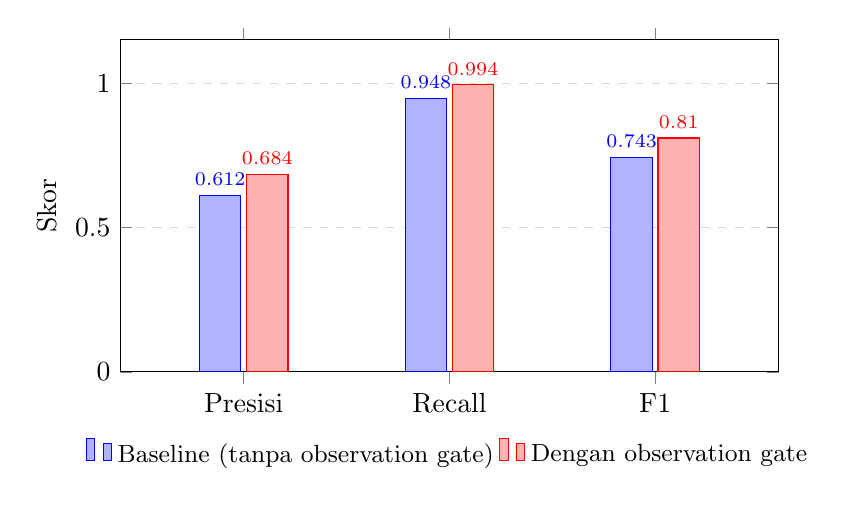
\begin{tikzpicture}
\begin{axis}[
    ybar,
    width=0.82\textwidth,
    height=58mm,
    bar width=15pt,
    ymin=0, ymax=1.15,
    ylabel={Skor},
    symbolic x coords={Presisi, Recall, F1},
    xtick=data,
    nodes near coords,
    nodes near coords style={font=\scriptsize, /pgf/number format/fixed,
                             /pgf/number format/precision=3},
    legend style={at={(0.5,-0.18)}, anchor=north, legend columns=2, font=\small,
                  draw=none},
    enlarge x limits=0.3,
    ymajorgrids=true,
    grid style={dashed, gray!30},
]
\addplot coordinates {(Presisi,0.612) (Recall,0.948) (F1,0.743)};
\addplot coordinates {(Presisi,0.684) (Recall,0.994) (F1,0.810)};
\legend{Baseline (tanpa observation gate), Dengan observation gate}
\end{axis}
\end{tikzpicture}
\caption{Ablasi \emph{observation gate}. Penggerbangan menaikkan presisi tanpa mengorbankan
\emph{recall} sehingga menghasilkan kenaikan $F_1$ neto.}
\label{fig:ablation}
\end{figure}

Sebagaimana diperlihatkan Gambar~\ref{fig:ablation}, \emph{observation gate} menaikkan $F_1$
sebesar $+0{,}067$ (dari 0,743 menjadi 0,810), yang disebabkan oleh kenaikan
presisi (rekomendasi berprasyarat numerik tidak lagi muncul bagi setiap pasien CCD) dengan
\emph{recall} yang praktis tidak berubah. Karena kedua konfigurasi berbagi \emph{baseline}
yang sama, ablasi ini mengisolasi kontribusi \emph{observation gate} itu sendiri. Ablasi ini tidak mengisolasi kontribusi wadah datanya. Pertanyaan apakah perolehan tersebut memang
menuntut FHIR merupakan pertanyaan yang terpisah dan diuji tersendiri pada
Subbab~\ref{sec:csv-gating}.

\subsection{Dari mana kenaikan tersebut berasal}
\label{sec:ablation-class}
Perlu dipahami angka pada Tabel~\ref{tab:ablation} dan Gambar~\ref{fig:ablation} merupakan angka rata-rata dari 68 rekomendasi sehingga sumber kenaikan angka tersebut perlu dilihat berdasarkan masing-masing rekomendasi.
Subbab~\ref{sec:disc-class} memilah 68 rekomendasi nonkontraindikasi menurut cara
masing-masing mempersempit kohort dan hanya 15 rekomendasi yang membawa prasyarat numerik
yang dinilai berbeda ketika penggerbangan dinyalakan. Ke-53 rekomendasi sisanya memberi
jawaban yang sama pada kedua keadaan sehingga mereka menurunkan rerata tanpa menyumbang
apa pun pada perubahan yang hendak diperlihatkan rerata itu. Tabel~\ref{tab:ablation-class} melaporkan keselarasan secara terpisah untuk
setiap kelas pada kedua lengan.

\begin{table}[h]
\centering
\caption{Keselarasan menurut kelas pembeda pada kedua lengan ablasi, rerata mikro dari kohort
876 pasien. Kelasnya mengikuti Subbab~\ref{sec:disc-class}: rekomendasi
\emph{universal} sama sekali tidak membawa mekanisme untuk mempersempit kohort,
\emph{concept-matched} mensyaratkan target kondisi lanjutan, \emph{value-gated} mensyaratkan
predikat numerik atas sebuah observasi, dan \emph{both} mensyaratkan keduanya sekaligus. Kedua
kelas yang tidak tergerbang identik pada kedua lengan hingga cacah satuannya; seluruh efek
ablasi hanya berdampak pada 15 rekomendasi yang tergerbang.}
\label{tab:ablation-class}
\footnotesize
\setlength{\tabcolsep}{4pt}
\begin{tabular}{lr|ccc|ccc}
\hline
& & \multicolumn{3}{c|}{\textbf{\emph{Baseline} (tanpa gerbang)}}
  & \multicolumn{3}{c}{\textbf{Dengan \emph{observation gate}}} \\
\textbf{Kelas} & \textbf{rek.} & \textbf{P} & \textbf{R} & \textbf{$F_1$}
                               & \textbf{P} & \textbf{R} & \textbf{$F_1$} \\
\hline
Universal        & 38 & 0,666 & 1,000 & 0,799 & 0,666 & 1,000 & 0,799 \\
Tercocok-konsep  & 15 & 0,676 & 0,915 & 0,777 & 0,676 & 0,915 & 0,777 \\
Tergerbang-nilai & \phantom{0}5 & 0,194 & 1,000 & 0,325
                                & \textbf{1,000} & \textbf{1,000} & \textbf{1,000} \\
Keduanya         & 10 & 0,038 & 0,006 & 0,011
                                & \textbf{1,000} & \textbf{1,000} & \textbf{1,000} \\
\hline
\textbf{Semua}   & 68 & 0,613 & 0,945 & 0,743 & 0,685 & 0,993 & 0,811 \\
\hline
\end{tabular}
\end{table}

Didapatkan empat hasil pembacaan hasil dari Tabel~\ref{tab:ablation-class}.

Pertama, kedua kelas yang tidak tergerbang \emph{identik} pada kedua lengan---bukan hanya
hampir sama, melainkan sama hingga ke cacah satuan \emph{true positive}, \emph{false positive},
dan \emph{false negative} ($22.158/11.130/0$ untuk kelas universal, $2.018/969/188$ untuk
kelas dengan konsep yang cocok). Oleh karena itu, 53 dari 68 rekomendasi tidak tersentuh dan
seluruh selisih $F_1$ yang dilaporkan berasal dari 15 rekomendasi sisanya. Hal ini merupakan
prediksi yang dapat difalsifikasi dari klasifikasi pada Subbab~\ref{sec:disc-class} dan
prediksi tersebut terbukti persis.

Kedua, kedua kelas yang tergerbang memperoleh manfaat dengan cara yang berlawanan. Bagi kelima rekomendasi
\emph{tergerbang-nilai}, penggerbangan merupakan mekanisme \emph{presisi}: tanpa
penggerbangan, rekomendasi tersebut muncul bagi setiap anggota kohort (849 \emph{true positive}
berbanding 3.531 \emph{false positive}, $P = 0{,}194$) dan dengan penggerbangan, rekomendasi
tersebut hanya muncul bila nilai terukur memenuhi predikatnya ($P = 1{,}000$), sementara
\emph{recall}-nya memang sudah sempurna. Bagi kelas \emph{keduanya}, penggerbangan justru sangat dominan sebagai mekanisme
\emph{recall}. Pada lengan \emph{baseline}, kesepuluh rekomendasi tersebut nyaris tidak
pernah muncul sama sekali (8 \emph{true positive} berbanding 1.263 \emph{false negative}, $R
= 0{,}006$) karena target kondisinya yang terkodekan saja jarang cocok. Predikat observasi
itulah yang sesungguhnya mengenali pasien yang dikenai rekomendasi tersebut.
Menggambarkan ablasi semata-mata sebagai perbaikan presisi menjadi keliru bagi dua pertiga rekomendasi yang terpengaruh.

Ketiga, kedua kelas yang tergerbang mencapai $P = R = 1{,}000$ setelah penggerbangan
dinyalakan. Nilai sempurna itu mengatakan sesuatu tentang urusan teknisnya, bukan tentang
seberapa sulit penilaian klinisnya. \emph{Observation gate} dan standar rujukan menerapkan ambang panduan klinis yang sama,
misalnya fraksi ejeksi 40\% atau kurang. Namun, keduanya membaca nilai pasien dari tempat
yang berbeda. Gerbang membacanya dari graf, sedangkan standar rujukan membacanya dari
\emph{bundle} FHIR mentah. Karena itu, kesepakatan pada setiap pasien
menunjukkan bahwa \emph{loader} membawa nilai-nilai tersebut tanpa mengubahnya. Hal itu tidak
menunjukkan bahwa ambangnya benar secara klinis sebab kedua sisi memang diberi ambang yang
sama sejak awal. Subbab~\ref{sec:shared-predicate} memastikan bahwa keduanya memang fungsi yang
sama, lalu mengukur seberapa besar bagian angka keselarasan yang bertumpu pada hal tersebut.

Keempat, lima dari sepuluh rekomendasi kelas \emph{both} bersifat \emph{tidak aktif}.
\texttt{TP:2}, \texttt{TP:3:1}, \texttt{TP:3:2}, \texttt{TP:4}, dan \texttt{TP:5} mencatat nol
\emph{true positive}, nol \emph{false positive}, dan nol \emph{false negative} pada \emph{kedua}
lengan sehingga tidak menyumbang apa pun pada kolom mana pun. Kelimanya digerbangi oleh satu
predikat yang sama---merokok aktif setiap hari---yang tidak dipenuhi satu pun pasien dalam
kohort: dari 876 pasien, 390 tercatat tidak pernah merokok,
237 sebagai mantan perokok, 249 sama sekali tidak membawa observasi
status merokok, dan 0 merupakan perokok aktif. Karena itu, baris \emph{both}
sepenuhnya ditentukan oleh lima rekomendasi yang aktif dan cacah yang dikutip di atas bagian dari
kelima rekomendasi tersebut, bukan bagian dari sepuluh lainnya. \texttt{LIPID:9} tidak aktif karena alasan
sejenis---tidak ada pasien kohort yang memenuhi konjungsinya---sehingga gerbang yang
diperolehnya ketika trigliserida dimuat tidak pernah terpakai.

Hal ini berlaku lebih luas daripada hanya sebatas pada kelas-kelas yang tergerbang. Sebanyak 22 dari
73 pengenal rekomendasi dalam berkas label rujukan tidak memiliki satu pun hasil
positif di seluruh kohort. Hal tersebut merupakan sifat dari penggunaan populasi sintetis, bukan akibat pengodeannya:
rekomendasinya terkodekan dengan benar dan akan menyala bila pasien yang relevan hadir. Namun, hal
tersebut tetap membatasi apa yang dapat ditunjukkan angka keselarasan ini dan kohort nyata akan
mengaktifkan subhimpunan yang berbeda serta mungkin lebih besar. Subbab~\ref{sec:module-yield} menunjukkan penyebab utamanya. Sebanyak 249 dari 876 pasien,
sekitar 28\%, berasal dari proses Synthea yang diperkaya penyakit. Rekam medis mereka hanya
membawa satu diagnosis penyakit jantung iskemik, satu temuan pencitraan jantung yang
abnormal, dan kadang riwayat \emph{bypass}, tanpa komorbiditas dan, selain fraksi ejeksi,
tanpa observasi apa pun.

Ada satu pilihan perataan (\emph{averaging}) yang berlaku di seluruh tabel ini. Angka-angkanya dirata-ratakan secara \emph{mikro}: seluruh
positif benar, positif salah, dan negatif salah pada kohort dijumlahkan lebih dahulu, lalu
rasionya dihitung sekali saja di akhir.

Pilihan yang lain, perataan \emph{makro}, menilai tiap pasien sendiri-sendiri lalu
merata-ratakan nilai itu. Cara tersebut tidak dapat dipakai di sini. Penyebabnya, seorang pasien dapat sama sekali tidak tersentuh oleh suatu kelas. Bagi pasien
itu, tidak ada yang dapat dijawab benar oleh sistem dan tidak ada pula yang dapat dijawab
salah sehingga ketiga cacahnya nol. Presisi, \emph{recall}, dan $F_1$-nya lalu ditetapkan
nol, bukan dibiarkan kosong. Nol itu masuk ke rerata seolah-olah
sistem gagal menangani pasien tersebut. Makin jarang suatu kelas, makin banyak pasien semacam
itu, dan makin turun pula angka makronya. Pada akhirnya, angka tersebut mengukur seberapa umum kelas itu, bukan seberapa baik sistem menanganinya.

Kelas tergerbang-nilai memperlihatkan hal ini pada ukuran penuhnya: makro $F_1 = 0{,}600$
berbanding nilai mikro $1{,}000$. Keduanya tidak saling bertentangan. Karena pada kelas itu
tidak ada satu pun positif salah maupun negatif salah, tiap pasien bernilai tepat satu atau
tepat nol sehingga angka makronya tidak lain adalah porsi kohort yang sama sekali memiliki
rekomendasi tergerbang-nilai---526 dari 876. Setiap pasien yang memang dikenai kelas tersebut
dinilai dengan sempurna. Itulah sebabnya seluruh angka per kelas yang dilaporkan di sini
dirata-ratakan secara mikro.

\subsection{Bagian mana yang dinilai secara independen}
\label{sec:shared-predicate}
Subbab~\ref{sec:oracle} memilah ketakbergantungan standar rujukan menjadi dua tingkatan. Subbab
ini melaporkan akibatnya terhadap angka yang dilaporkan.

Bagi 15 rekomendasi tergerbang-observasi, predikat sistem dan aturan standar rujukan merupakan
fungsi yang sama. Hal itu diperiksa secara empiris, bukan sekadar dibaca dari kodenya: kedua
sisi dievaluasi atas 876 vektor ciri kohort yang sesungguhnya dan atas 200.000 vektor sintetis
yang diarahkan ke tiap ambang yang diujinya, termasuk nilai yang hilang, dan tidak satu pun
dari 200.876 perbandingan itu berbeda. Karena itu, presisi dan \emph{recall} sebesar $1{,}000$
pada kedua kelas tergerbang tidak dapat dibaca sebagai penilaian atas ketepatan aturannya.

Tabel~\ref{tab:shared-predicate} memisahkan keduanya.

\begin{table}[h]
\centering
\caption{Keselarasan panduan klinis dipilah menurut tingkatan ketakbergantungan standar
rujukannya, dirata-ratakan secara mikro pada kohort 876 pasien.}
\label{tab:shared-predicate}
\begin{tabular}{lrcccrrr}
\hline
\textbf{Bagian} & \textbf{rek.} & \textbf{Presisi} & \textbf{\emph{Recall}} & \textbf{$F_1$} &
\textbf{tp} & \textbf{fp} & \textbf{fn} \\
\hline
Seluruhnya            & 68 & 0,685 & 0,993 & 0,811 & 26.296 & 12.099 & 188 \\
Predikat bersama      & 15 & 1,000 & 1,000 & 1,000 & 2.120 & 0 & 0 \\
Logika tak bergantung & 53 & 0,666 & 0,992 & 0,797 & 24.176 & 12.099 & 188 \\
\hline
\end{tabular}
\end{table}

Bagian yang dinilai penilai yang benar-benar tidak bergantung mencakup 53 dari 68 rekomendasi
dan mencatat presisi $0{,}666$ serta $F_1$ $0{,}797$. Menyingkirkan kelima belas rekomendasi
berpredikat bersama karenanya menurunkan presisi sebesar $0{,}018$ dan $F_1$ sebesar $0{,}013$;
sebanyak $8{,}1\%$ dari seluruh \emph{true positive} berasal dari bagian berpredikat bersama
tersebut. Dengan kata lain, angka utama tidak ditopang oleh bagian yang berpredikat bersama
dan kesimpulan mengenai keselarasan tetap berlaku bila bagian itu dihapus seluruhnya.

Ablasinya berbeda halnya dan hal itu perlu dinyatakan terus terang. Hanya kelas
tergerbang-nilai dan kelas keduanya yang berubah di antara kedua lengan ablasi dan keduanya
justru merupakan kelima belas rekomendasi berpredikat bersama itu. Seluruh perolehan ablasi
karenanya terukur pada rekomendasi yang standar rujukannya menerapkan aturan yang sama dengan
sistemnya. Perolehan itu tetap merupakan perubahan nyata pada perilaku sistem. Tanpa gerbang,
rekomendasi berprasyarat numerik muncul bagi pasien yang tidak memenuhi prasyarat yang
dinyatakan panduan klinis dan hal itu tetap merupakan cacat, siapa pun penilainya. Meski
begitu, perolehan itu mengukur kesetiaan implementasi, bukan keabsahan klinis. Standar rujukannya merupakan
penilai yang tidak bergantung atas nilai yang disuapkan ke aturannya, bukan atas aturannya
sendiri.

\subsection{Apakah perolehan tersebut menuntut FHIR?}
\label{sec:csv-gating}
Ablasi pada Tabel~\ref{tab:ablation} mengisolasi kontribusi \emph{observation gate}, bukan
kontribusi wadah datanya. Kedua hal itu mudah tertukar. Bab~I melandaskan rancangan FHIR-native
pada pembandingan terhadap ekspor tabular terdatarkan sehingga dari situ mudah disimpulkan
bahwa gerbangnya menjadi mungkin justru karena FHIR. Simpulan tersebut semula dinyatakan, bukan
diukur. Subbab ini mengukurnya.

Pengujiannya berupa lengan ketiga. Gerbang yang sama dibangun ulang dengan hanya membaca ekspor
CSV Synthea---\texttt{observations.csv} dan \texttt{conditions.csv}---tanpa menyentuh
\emph{bundle} maupun graf. Logika pencocokan untaiannya, ambangnya, serta aturan agregasinya
disalin apa adanya dari \texttt{silver\_oracle.py} sehingga ketidaksepakatan yang muncul dapat
diatributkan pada wadah datanya dan bukan pada perbedaan logika klinis. Itulah maksud
perancangan eksperimen ini.

Pembandingnya adalah jalur \emph{bundle} FHIR, bukan jalur graf. Untuk keperluan ini keduanya
setara: kelima belas rekomendasi tergerbang-observasi mencatat presisi dan \emph{recall}
$1{,}000$ terhadap standar rujukan pada seluruh kohort, sebagaimana dilaporkan
Subbab~\ref{sec:ablation-class}, sehingga keputusan gerbang pada graf dan keputusan standar
rujukan sudah bersesuaian seluruhnya. Dengan demikian, mereproduksi standar rujukan berarti
mereproduksi gerbang pada graf pula, tanpa memerlukan Neo4j.

Tabel~\ref{tab:csv-gating} melaporkan hasilnya.

\begin{table}[h]
\centering
\caption{Gerbang observasi yang dibangun dari \emph{bundle} FHIR dibandingkan yang dibangun dari
ekspor CSV, untuk 15 rekomendasi tergerbang-observasi pada 876 pasien.}
\label{tab:csv-gating}
\begin{tabular}{lcccrrr}
\hline
\textbf{Sumber data} & \textbf{Presisi} & \textbf{\emph{Recall}} & \textbf{$F_1$} &
\textbf{tp} & \textbf{fp} & \textbf{fn} \\
\hline
\emph{Bundle} FHIR & 1,000 & 1,000 & 1,000 & 2.120 & 0 & 0 \\
Ekspor CSV         & 1,000 & 1,000 & 1,000 & 2.120 & 0 & 0 \\
\hline
\end{tabular}
\end{table}

Dari 13.140 keputusan gerbang---876 pasien dikali 15 rekomendasi---tidak satu pun berbeda di
antara kedua sumber data tersebut. Cacah 2.120 itu sendiri merupakan penjumlahan \emph{true
positive} kedua kelas tergerbang pada lengan bergerbang Tabel~\ref{tab:ablation-class}---849
bagi kelas tergerbang-nilai dan 1.271 bagi kelas keduanya---sehingga kesamaan angkanya sekaligus
menjadi pemeriksaan bahwa rekonstruksinya memang mengukur hal yang sama. Kohortnya pun bernasib
serupa: kode SNOMED~CT
\texttt{414545008} pada \texttt{conditions.csv} memilih tepat 876 pasien yang sama dengan
gerbang pada graf.

Dua hal yang benar-benar hilang pada ekspor itu dapat diukur dan keduanya ternyata tidak
mengubah keputusan apa pun. Pertama, ekspornya membulatkan nilai observasi ke satu angka di
belakang koma. Sebanyak 1.990 nilai karenanya berbeda antara kedua jalur, dengan selisih
terbesar $0{,}05$. Tiga di antaranya berpindah sisi terhadap sebuah ambang. Satu kasus fraksi
ejeksi ($39{,}999$ menjadi $40{,}0$) sebenarnya bukan paparan sama sekali sebab predikat yang
memakainya menguji ``$\le 40$'' dan ``$> 40$''; kedua nilai itu menjawabnya secara sama. Dua kasus trigliserida ($149{,}97$ dan $149{,}96$, keduanya menjadi $150{,}0$) merupakan
paparan yang sesungguhnya karena klausa ``$150 \le$ trigliserida'' berbalik menjadi benar.
Namun, \texttt{LIPID:9} juga mensyaratkan LDL di bawah 100 dan syarat itu tidak terpenuhi
pada kedua pasien tersebut ($130{,}1$ dan $148{,}6$). Karena itu, tidak ada rekomendasi yang berubah.

Kedua, panel tekanan darahnya memang tidak terbawa, persis sebagaimana dinyatakan
Subbab~\ref{sec:flattening}. Namun, pemulihannya ternyata tidak menuntut penerkaan. Kolom
\texttt{ENCOUNTER} terisi pada seluruh baris observasi sehingga 17.177 pasang sistolik dan
diastolik pada kohort ini dapat dirakit kembali seluruhnya tanpa menyisakan satu baris pun yang
tak berpasangan. Perakitan ulang itu merupakan biaya, bukan penghalang.

Simpulan yang dapat ditarik karenanya lebih sempit daripada yang semula dinyatakan Bab~I.
Perolehan presisinya nyata dan tidak berubah: \emph{observation gate} tetap menaikkan $F_1$
sebesar $+0{,}067$. Namun, bukti tidak mendukung atribusi perolehan itu kepada wadah FHIR secara khusus. Perolehan itu sesungguhnya dihasilkan oleh pemuatan nilai observasi numerik sebagai data kelas satu. FHIR menjadikannya langsung; ekspor tabular Synthea memungkinkannya pula,
dengan tambahan satu langkah perakitan ulang dan dengan ketelitian satu angka di belakang koma.
Pembedaan itu penting karena menentukan apa yang boleh diklaim. Klaim yang sah bukanlah
bahwa FHIR diperlukan, melainkan bahwa observasi numerik diperlukan. FHIR merupakan cara
yang paling langsung untuk memperolehnya.

Jangkauan simpulan ini perlu dinyatakan secara tegas. Pengujian ini menunjukkan bahwa ekspor CSV Synthea membawa cukup data bagi sembilan kode LOINC yang dipakai gerbang pada
korpus ini. Pengujian ini tidak menunjukkan kesetaraan CSV dan FHIR secara umum dan tidak pula
menjangkau ekspor tabular dari sistem lain, yang belum tentu menyertakan kunci rujukan seperti
\texttt{ENCOUNTER}. Hal-hal yang tetap hilang pada ekspor tersebut---\texttt{status}
\emph{resource}, sistem kode pada nilai observasi, dan identitas panelnya---dibahas pada
Subbab~\ref{sec:flattening}; ketiganya tidak terpakai oleh gerbang ini, tetapi ketidakterpakaian
itu merupakan sifat korpus ini, bukan sifat rancangannya.

\section{Validasi \emph{Silver Standard} terhadap \emph{Gold Standard}}
\label{sec:gold}

Untuk memvalidasi \emph{silver standard} yang dihasilkan otomatis, 30 pasien
dilabeli secara manual guna membentuk \emph{gold standard} lalu dibandingkan terhadap label
\emph{silver}. Kesepakatannya mencapai 99,5\% (2.150 dari 2.160 sel)
dengan Cohen's $\kappa = 0{,}991$ (interval kepercayaan 95\% 0,984---0,996;
Subbab~\ref{sec:kappa-ci}), yang menunjukkan kesepakatan hampir sempurna.
Hasil inilah yang memvalidasi bahwa sisa evaluasi dapat dilakukan. Karena
\emph{silver standard} mereproduksi pertimbangan manusia hampir secara persis pada sampel
tempat keduanya tersedia, angka keselarasan yang dihitung terhadapnya atas keseluruhan
kohort 876 pasien bertumpu pada rujukan yang tervalidasi, bukan rujukan yang diasumsikan.
Inilah standar justifikasi untuk menggantikan anotasi manual dengan label yang dihasilkan
otomatis pada skala besar \cite{rebholz2011,nogues2022}. Pelabel dan rubriknya diuraikan pada Subbab~\ref{sec:goldlabel}.

\subsection{Ketidaksepakatan yang tersisa}
Sepuluh dari 2.160 sel yang dibandingkan tidak sepakat. Kesepuluhnya dirinci satu per satu
pada Tabel~\ref{tab:disagreements} karena sebarannya lebih informatif
daripada jumlahnya.

\begin{table}[h]
\centering
\caption{Seluruh ketidaksepakatan \emph{silver}-\emph{gold}. ``Lebih'' berarti \emph{silver
standard} menandai sebuah rekomendasi berlaku, sedangkan penilai manusia tidak; ``kurang''
sebaliknya.}
\label{tab:disagreements}
\footnotesize
\begin{tabular}{llccl}
\hline
\textbf{Pasien} & \textbf{Rekomendasi} & \textbf{COR} & \textbf{\emph{Silver}/\emph{Gold}}
& \textbf{Arah} \\
\hline
\texttt{cbf432fc} & \texttt{APT:6}    & 2b & 1/0 & lebih  \\
\texttt{6595b70f} & \texttt{BB:2}     & 1  & 0/1 & kurang \\
\texttt{1db4196c} & \texttt{BPM:3}    & 1  & 1/0 & lebih  \\
\texttt{05e41fe3} & \texttt{LIPID:2}  & 1  & 1/0 & lebih  \\
\texttt{22f599b6} & \texttt{LIPID:2}  & 1  & 1/0 & lebih  \\
\texttt{2b050f16} & \texttt{LIPID:2}  & 1  & 0/1 & kurang \\
\texttt{2b050f16} & \texttt{LIPID:3}  & 1  & 1/0 & lebih  \\
\texttt{04287b67} & \texttt{LIPID:5}  & 2a & 0/1 & kurang \\
\texttt{cbf432fc} & \texttt{LIPID:5}  & 2a & 0/1 & kurang \\
\texttt{227e76d8} & \texttt{LIPID:10} & 2b & 0/1 & kurang \\
\hline
\end{tabular}
\end{table}

Tiga sifat dari himpunan ini penting. Pertama, ketidaksepakatannya \emph{seimbang persis}: lima
penandaan berlebih dan lima penandaan kurang, terhadap 1.080 sel yang keduanya menandai sebagai
rekomendasi yang dapat diberlakukan dan 1.070 sel yang keduanya menandai sebagai tidak dapat diberlakukan. \emph{Silver standard} karenanya tidak
secara sistematis lebih longgar maupun lebih ketat daripada pelabel manusia---dan sifat inilah
yang paling mengancam penggunaan rujukan otomatis sekaligus paling sulit ditetapkan melalui
argumen semata.

Kedua, ketidaksepakatannya \emph{terpusat}, bukan tersebar: tujuh dari sepuluh menyangkut
rekomendasi lipid (\texttt{LIPID:2} tiga kali, \texttt{LIPID:5} dua kali, serta
\texttt{LIPID:3} dan \texttt{LIPID:10} masing-masing sekali). Di sinilah teks panduan klinis paling
sulit dimekaniskan. \texttt{LIPID:2} berlaku ketika terapi statin intensitas tinggi
``dikontraindikasikan atau tidak ditoleransi''---intoleransi tidak terepresentasikan dalam
rekam medis berkode sehingga \emph{silver standard} maupun penilai manusia sama-sama harus
menyimpulkannya. \texttt{LIPID:5} berlaku bagi pasien yang ``dinilai berisiko sangat tinggi'',
sebuah komposit yang secara eksplisit terdapat di panduan klinis untuk menjadi pertimbangan bagi klinisi.
\texttt{LIPID:10} mensyaratkan secara bersamaan, bahwa pasien \emph{tidak} berisiko sangat
tinggi, sedang menjalani terapi statin ``yang dapat ditoleransi secara maksimal'', dan memiliki
LDL-C~$\geq$~70~mg/dL. Klausa-klausa inilah yang persis menjadi sebab kebijakan
klausa-tak-terpastikan pada standar rujukan (Subbab~\ref{sec:oracle}) dipilih menjadi abstain. Galat
yang tersisa karenanya terlokalisasi pada prasyarat yang secara tidak terhindarkan bersifat
pertimbangan, alih-alih tersebar ke seluruh himpunan rekomendasi.

Ketiga, kesepuluh sel tersebut mewakili \emph{kurang dari sepuluh pertimbangan yang saling
bebas}. Pasien \texttt{2b050f16} menyumbang dua di antaranya---penandaan kurang pada
\texttt{LIPID:2} dan penandaan lebih pada \texttt{LIPID:3}---yang secara bersamaan paling masuk
akal dibaca sebagai satu ketidaksepakatan mengenai intensitas statin yang tercatat pada dua
sel; pasien \texttt{cbf432fc} juga menyumbang dua. Cohen's $\kappa$ memperlakukan setiap sel
sebagai saling bebas sehingga nilai yang dilaporkan sedikit \emph{menurunkan} tingkat
kesepakatan yang sebenarnya.

\subsection{Ketidakpastian $\kappa$ dan kecukupan 30 pasien}
\label{sec:kappa-ci}
Ketidakbebasan yang sama juga menyangkut ketidakpastian $\kappa$. Sebanyak 2.160 sel yang
dibandingkan mengelompok dalam 30 pasien dan rekam medis seorang pasien menentukan seluruh
labelnya sekaligus. Karena itu, interval kepercayaan yang semestinya adalah interval yang
mencuplik ulang \emph{pasien}, bukan sel (Subbab~\ref{sec:goldlabel}).
Tabel~\ref{tab:kappa-ci} melaporkan keduanya agar perbedaannya dapat dilihat.

\begin{table}[h]
\centering
\caption{Interval kepercayaan 95\% bagi Cohen's $\kappa$ \emph{silver}-\emph{gold}, dari
10.000 replikasi \emph{bootstrap} untuk tiap satuan pencuplikan ulang.}
\label{tab:kappa-ci}
\begin{tabular}{lcc}
\hline
\textbf{Satuan pencuplikan ulang} & \textbf{Batas bawah} & \textbf{Batas atas} \\
\hline
Sel, dengan mengandaikan saling bebas & 0,984 & 0,996 \\
Pasien (\emph{bootstrap} klaster)      & 0,984 & 0,996 \\
\hline
\end{tabular}
\end{table}

Kedua cara menghasilkan interval yang sama, yaitu 0,984 hingga 0,996. Penyebabnya adalah
sebaran ketidaksepakatannya. Kesepuluh ketidaksepakatan tersebar pada 8 dari 30 pasien dan
tidak ada pasien yang menyumbang lebih dari dua. Efek desain (\emph{design effect})-nya hanya
1,04 sehingga pengelompokan per pasien nyaris tidak menambah ketidakpastian. Taksiran
\emph{jackknife} yang membuang satu pasien setiap kali menghasilkan $\kappa$ antara 0,990 dan
0,992. Dengan demikian, tidak ada satu pasien pun yang menopang angka tersebut.

Nilai $\kappa$ juga tidak digelembungkan oleh prevalensi label. Label positif mencakup 1.085 dari
2.160 sel pada kedua standar (50,2\%), indeks prevalensinya 0,005, dan indeks biasnya nol
karena ketidaksepakatannya seimbang lima banding lima. Kesepakatan yang diharapkan secara
kebetulan karenanya sekitar 0,500 dan $\kappa$ praktis sama dengan PABAK, yaitu 0,991
\cite{byrt1993}.

Jawaban atas pertanyaan apakah 30 pasien cukup bergantung pada klaim yang hendak didukung.
Untuk klaim bahwa \emph{silver standard} sepakat hampir sempurna dengan pelabelan manual, 30
pasien cukup. Batas bawah intervalnya, 0,984, jauh di atas ambang 0,80 \cite{landis1977} dan
tidak satu pun dari 10.000 replikasi jatuh di bawah 0,95. Untuk klaim yang lebih halus,
misalnya bahwa $\kappa$ bernilai 0,99 dan bukan 0,98, 30 pasien tidak cukup dan klaim
semacam itu tidak dibuat.

Interval ini memiliki dua batas. Pertama, interval ini hanya menggambarkan pasien seperti
ketiga puluh pasien tersebut, yang dipilih secara purposif dan condong pada rekam yang paling
kompleks (Subbab~\ref{sec:gate}). Kedua, interval ini tidak menjawab keterbatasan pelabel
tunggal sebab pencuplikan ulang tidak dapat menghadirkan penilai kedua
(Subbab~\ref{sec:limitations}).

\section{Deteksi Keamanan}
\label{sec:safety-detection}

Deteksi keamanan kontraindikasi dievaluasi atas 151 tanda keamanan yang
dilabeli manual (Tabel~\ref{tab:safety}).

\begin{table}[h]
\centering
\caption{Deteksi keamanan kontraindikasi: pencocokan unary versus tergerbang-populasi.}
\label{tab:safety}
\begin{tabular}{lccc}
\hline
\textbf{Varian} & \textbf{Presisi} & \textbf{\emph{Recall}} & \textbf{$F_1$} \\
\hline
Unary (mengonsumsi obat yang dikontraindikasikan) & 0,139 & $\approx$1,000 & --- \\
Tergerbang-populasi (obat \emph{dan} kondisi populasinya) & 1,000 & 0,095 & 0,174 \\
\hline
\end{tabular}
\end{table}

Hasil ini menunjukkan adanya \emph{trade-off}, bukan kegagalan yang dapat diperbaiki dari kode. Pertama, pencocokan
\emph{unary} tidak pernah melewatkan kontraindikasi yang memang dapat dijangkau, tetapi \emph{over-flag},
sedangkan penggerbangan populasi presisinya sempurna, tetapi hanya memulihkan sebagian kecil
kontraindikasi yang kondisi populasinya dapat digerbangi secara struktural. Kedua, yang terlewat
adalah kontraindikasi yang didefinisikan melalui negasi dan yang bersifat konjungtif, yang
tidak dapat diungkapkan oleh skema saja.

Di luar \emph{trade-off} biner tersebut, rekomendasi NSAID kronis (\texttt{APT:10}) dinilai berdasarkan
varian ketiga, yaitu \emph{tergerbang-kronisitas}, yang hanya muncul bila graf menilai
penggunaan NSAID sebagai kronis berdasarkan status obat yang kategoris dan cacah periode penggunaan
berulang. Terhadap tanda keamanan yang dilabeli manual, varian ini mencapai presisi
0,909 dan \emph{recall} 0,526 (tp $=10$, fp $=1$,
fn $=9$)---sangat presisi, tetapi hanya memulihkan sekitar separuh kasus yang benar-benar
kronis. Kasus yang terlewat justru kasus yang menjadi kronis \emph{hanya} melalui satu periode
penggunaan panjang, misalnya peresepan ibuprofen selama 101 hari dan 111 hari. Graf tidak
dapat melihat kasus semacam itu karena ekspor FHIR tidak memuat tanggal berhenti
(Subbab~\ref{sec:chronicity}). Ini bukan artefak yang dapat diperbaiki dengan melakukan 
\emph{tuning}, melainkan \emph{trade-off}
dari rancangan FHIR-native: status obat yang kategoris memulihkan lengan ``sedang berjalan''
dan lengan ``banyak periode penggunaan'' dari aturan kronisitas, tetapi lengan berbasis durasi secara
struktural tidak dapat dipulihkan dari FHIR semata.

\section{\emph{Faithfulness} Ringkasan}
\label{sec:faithfulness}

\emph{Grounded briefing} dibangkitkan untuk 30 pasien, yaitu sampel yang sama dengan sampel
\emph{gold standard}, lalu diperiksa secara otomatis terhadap fakta hasil penelusurannya.
Lima di antaranya dibangkitkan lebih dahulu dan menjadi dasar laporan awal penelitian ini.
Dua puluh lima sisanya dibangkitkan kemudian dengan alur dan model yang sama.

Pemeriksaan itu menguji empat hal. Pertama, setiap pengenal rekomendasi yang disebut
ringkasan harus terdapat pada fakta. Kedua, setiap PMID yang disebut juga harus terdapat pada
fakta. Ketiga, setiap rekomendasi yang berlaku dan setiap tanda keamanan pada fakta harus
disebut. Keempat, ringkasan tidak boleh menyatakan bahwa pasien memerlukan antikoagulan oral
bila tidak ada antikoagulan pada daftar obatnya. Pernyataan bersyarat, misalnya ``bila
memerlukan antikoagulan oral'', tetap diperbolehkan.

Seluruh 30 ringkasan lolos keempat uji tersebut: nol rekomendasi yang dikarang, nol PMID
yang dikarang, nol rekomendasi yang terlewat, dan nol klaim antikoagulan yang berlebih.

Uji keempat perlu dilaporkan beserta riwayatnya. Pada penerapan pertamanya atas 30
ringkasan, uji itu menandai sepuluh baris pada empat ringkasan sebagai klaim berlebih. Kesepuluhnya
ternyata \emph{false positive} dengan bentuk yang sama. Bagian penelusuran provenans pada
ringkasan menulis ``\emph{conditional on oral anticoagulation need (not confirmed in current
medications)}'' dan pola pemeriksaannya menangkap kata \emph{on} di dalam
\emph{conditional on}. Uji itu kemudian dibatasi pada bagian ringkasan yang ditindaklanjuti
pembaca. Kemunculan pada bagian provenans tetap dihitung dan dilaporkan, bukan dibuang.
Perbaikan itu dilakukan \emph{sesudah} keluarannya terlihat dan hal itu perlu dinyatakan.
Hasil lima dari lima pada laporan awal bertahan sebagian karena kelima ringkasan pertama
kebetulan merumuskan pernyataan bersyaratnya dalam bentuk yang dikenali pemeriksaan.

Keempat uji itu tidak sama dengan \emph{faithfulness} makna. Penelusuran yang deterministik
menjamin bahwa fakta yang diterima model bahasa persis dan dapat direproduksi. Penelusuran itu
juga membuat butir yang dapat disitasi dapat diperiksa terhadap himpunan fakta yang tertutup.
Namun, penelusuran itu tidak menjamin bahwa setiap kalimat yang dirumuskan model setia pada
fakta tersebut. Model masih dapat, misalnya, melekatkan kondisi atau obat yang tidak ada pada
fakta kepada pasien, keliru menyebut alasan sebuah rekomendasi berlaku, atau menyatakan
rekomendasi berkelas lemah seolah-olah wajib. Kecuali pola antikoagulan, tidak satu pun
kekeliruan semacam itu ditangkap oleh pemeriksaan ini. Karena itu, yang dilaporkan di sini
adalah \emph{faithfulness} pada tingkat sitasi dan kelengkapan, ditambah satu pola klaim
berlebih. \emph{Faithfulness} makna setiap kalimat masih memerlukan pembacaan manusia dan hal
itu dicatat sebagai keterbatasan pada Subbab~\ref{sec:limitations}.

Bagian keamanan pada ringkasan menerapkan gerbang kronisitas berbasis graf yang sama seperti
pada lapisan rekomendasi. Karena itu, bagi pasien yang penggunaan NSAID-nya kronis
\emph{hanya} melalui durasi, tanda NSAID kronis tidak ditampilkan alih-alih dinyatakan tanpa
dukungan. Penghilangan tersebut konsisten dengan angka \emph{recall} deteksi keamanan yang
dilaporkan pada Subbab~\ref{sec:safety-detection} dan dapat dilacak kepadanya.

Lampiran~\ref{app:briefing} memuat satu ringkasan secara utuh dan tanpa suntingan sehingga apa yang sebenarnya diperiksa dapat dibaca langsung, bukan sekadar diuraikan.

\section{Telaah Klinisi}
\label{sec:clinician}

Subbab ini melaporkan penilaian klinisi atas ketepatan rekomendasi yang dikeluarkan sistem
(Subbab~\ref{sec:clinician-method}). Tabel~\ref{tab:clinician} merangkum sebaran penilaian
menurut penilai dan jenis rekomendasi. Rekomendasi antitrombotik mencakup terapi antiplatelet
dan antikoagulan (\texttt{APT}), sedangkan rekomendasi penyekat beta mencakup peninjauan ulang
dan tanda cek/stop penyekat beta (\texttt{BB}).

\begin{table}[h]
\centering
\caption{Sebaran penilaian klinisi menurut penilai dan jenis rekomendasi. Persentase dihitung
terhadap baris yang dinilai penilai tersebut.}
\label{tab:clinician}
\small
\begin{tabular}{llrrrr}
\hline
\textbf{Penilai} & \textbf{Rekomendasi} & \textbf{Baris} & \textbf{Tepat} &
\textbf{Belum tepat} & \begin{tabular}[b]{@{}r@{}}\textbf{Tidak dapat}\\\textbf{dinilai}\end{tabular} \\
\hline
A (SpJP)        & Antitrombotik & 101 & 52  & 46 & 3  \\
                & Penyekat beta  & 40  & 35  & 5  & 0  \\
                & Lainnya       & 106 & 105 & 1  & 0  \\
                & Seluruhnya    & 247 & 192 (77,7\%) & 52 (21,1\%) & 3 (1,2\%) \\
\hline
B (dokter umum) & Antitrombotik & 66  & 19  & 32 & 15 \\
                & Penyekat beta  & 25  & 9   & 1  & 15 \\
                & Lainnya       & 69  & 69  & 0  & 0  \\
                & Seluruhnya    & 160 & 97 (60,6\%) & 33 (20,6\%) & 30 (18,8\%) \\
\hline
C (SpJP senior) & Seluruhnya    & 16  & 6   & 5  & 5  \\
\hline
\end{tabular}
\end{table}

Penilai~A menilai 192 dari 247 rekomendasi tepat (77,7\%; interval kepercayaan 95\% per
pasien 74,4---81,1\%). Penilai~B menilai 97 dari 160 rekomendasi tepat (60,6\%;
56,1---67,3\%). Selisih keduanya terutama berasal dari pilihan ``Tidak dapat dinilai'', yang
dipakai penilai~B pada 30 baris dan penilai~A hanya pada 3 baris. Bila baris itu
dikecualikan, proporsi ``Tepat'' keduanya lebih berdekatan, yaitu 78,7\% dan 74,6\%.

Penilaian yang tidak tepat terpusat pada rekomendasi antitrombotik. Sebanyak 46 dari 52
penilaian ``Belum tepat'' oleh penilai~A dan 32 dari 33 oleh penilai~B jatuh pada rekomendasi
tersebut. Sebaliknya, di luar rekomendasi antitrombotik dan penyekat beta, penilai~A menilai
105 dari 106 baris tepat dan penilai~B menilai seluruh 69 barisnya tepat. Kelompok itu
mencakup target tekanan darah dan antihipertensi lini pertama, rujukan rehabilitasi jantung,
tata laksana berat badan, penghambat SGLT2, serta tanda keamanan nitrat bersama penghambat
PDE5. Tiga rekomendasi berpredikat bersama (Subbab~\ref{sec:shared-predicate}) termasuk di
dalamnya, yaitu \texttt{WM:2}, \texttt{WM:3}, dan \texttt{SGLT2:4}. Ketiganya dinilai tepat
pada seluruh 30 baris penilai~A dan seluruh 20 baris penilai~B. Bagi ketiga rekomendasi itu,
penilaian klinisi memberikan pengujian atas aturannya yang tidak dapat diberikan standar
rujukan.

Penilai~A dan penilai~B sama-sama menilai 159 baris pada 10 pasien. Kesepakatan teramatinya
65,4\% (interval kepercayaan 95\% per pasien 58,8---73,9\%), dengan Cohen's
$\kappa = 0{,}29$ (0,18---0,41) dan PABAK 0,48. Nilai $\kappa$ tersebut tergolong
kesepakatan yang cukup \cite{landis1977}. Kesepakatan itu tidak merata. Pada 69 baris di luar
rekomendasi antitrombotik dan penyekat beta, keduanya sepakat pada 68 baris (98,6\%). Pada 90
baris antitrombotik dan penyekat beta, keduanya hanya sepakat pada 36 baris (40,0\%). Sebanyak
27 dari 55 ketidaksepakatan melibatkan pilihan ``Tidak dapat dinilai'' oleh penilai~B.

Saran yang ditulis penilai menunjukkan sumber ketidaksepakatan tersebut. Penilai~A tidak
menuliskan saran. Hampir seluruh pilihan ``Tidak dapat dinilai'' oleh penilai~B menanyakan
informasi yang tidak ditampilkan kesimpulan. Informasi itu berupa fraksi ejeksi dan status
gagal jantung pada rekomendasi penyekat beta serta risiko perdarahan pada perpanjangan terapi
antiplatelet ganda dan penambahan \emph{vorapaxar}. Pada tiga rekomendasi antikoagulan bersyarat
(\texttt{APT:11}---\texttt{APT:13}), penilai~B memilih ``Belum tepat'' pada 23 dari 24 baris.
Sebagai gantinya, penilai~B mengusulkan rangkaian yang berbeda, yaitu terapi tiga obat selama satu minggu, lalu DOAC
bersama clopidogrel hingga satu tahun, kemudian DOAC jangka panjang. Penilai~A menilai 13 dari
15 tanda cek/stop clopidogrel (\texttt{APT:7}) belum tepat, sedangkan penilai~B menilai 5 dari
11 belum tepat. Saran penilai~B pada baris tersebut menolak penghentian clopidogrel: pasien
pascainfark dinilai masih memerlukan terapi antiplatelet ganda atau clopidogrel tunggal bila
risiko perdarahannya tinggi.

Penilai~C menilai 6 dari 16 rekomendasi bagi pasien~1 tepat. Sarannya memperlihatkan
keterbatasan lembar telaah. Penilai~C memilih ``Tidak dapat dinilai'' pada dua tanda
cek/stop, yaitu clopidogrel dan nitrogliserin, karena kedua obat itu tidak tercantum pada
kesimpulan, padahal keduanya terdapat pada rekam medis pasien. Pilihan yang sama diberikan
pada tiga rekomendasi antikoagulan bersyarat karena pasien tidak memiliki indikasi
antikoagulan. Kedua tanda cek/stop penyekat beta dinilai belum tepat karena menurut penilai~C
pasien memerlukan penyekat beta. Pada pasien~1, penilai~C sepakat dengan penilai~A pada 6 dari
16 baris dan dengan penilai~B juga pada 6 baris; ketiganya sepakat penuh pada 5 baris.

Secara keseluruhan, klinisi menilai sebagian besar rekomendasi sistem sebagai sudah tepat
bagi pasiennya. Penilai~A, SpJP yang menilai paling banyak pasien (15 pasien), menyatakan
77,7\% rekomendasi sebagai sudah tepat. Pada penilai~B, seorang dokter umum, proporsi
rekomendasi yang dinilai sudah tepat lebih rendah karena lebih banyak rekomendasi yang
ditandainya ``Tidak dapat dinilai''. Hampir seluruh rekomendasi yang bukan mengenai
antitrombotik dan penyekat beta dinilai sudah tepat dengan kesepakatan penilai yang tinggi.
Sebaliknya, sebagian besar penilaian ``Belum tepat'' jatuh pada rekomendasi antitrombotik.
Pada rekomendasi penyekat beta, ketidaksepakatan antarpenilai hampir seluruhnya berasal dari
pilihan ``Tidak dapat dinilai''. Penilai~B menambahkan catatan bahwa informasi mengenai
fraksi ejeksi dan status gagal jantung diperlukan agar rekomendasi tersebut dapat dinilai.
Karena itu, kelompok rekomendasi mengenai antitrombotik dan penyekat beta menunjukkan
kesamaan hasil penilaian, yaitu bahwa rekomendasi tersebut bergantung pada informasi yang
tidak disajikan oleh kesimpulan sistem, seperti waktu sejak sindrom koroner akut, risiko
perdarahan, indikasi antikoagulan, fraksi ejeksi, dan status gagal jantung. Dengan demikian,
telaah ini menunjukkan bahwa rekomendasi sistem umumnya dinilai sudah tepat oleh klinisi.
Telaah ini juga menjelaskan bagian yang perlu diperbaiki terlebih dahulu, yaitu rekomendasi
antitrombotik dan penyekat beta beserta penjelasan informasi yang menjadi dasarnya.

\section{Perbandingan dengan Penelitian Terdahulu}
\label{sec:prior-work}

Subbab ini membandingkan hasil penelitian terhadap sistem yang telah diterbitkan sebelumnya.
Tabel~\ref{tab:prior-systems} membandingkannya menurut lima dimensi yang membedakan penelitian
ini: sumber data, apakah terminologi dijembatani ke dalam ruang konsep bersama, apakah panduan
klinis dikodekan sebagai lapisan yang dapat dikueri, apakah keluarannya dievaluasi terhadap
rujukan yang independen, dan apakah teks yang dihasilkan diperiksa \emph{faithfulness}-nya
secara mekanis.

\begin{table}[h]
\centering
\caption{Perbandingan dengan pendukung keputusan klinis berbasis \emph{knowledge graph} dan
FHIR terdahulu.}
\label{tab:prior-systems}
\footnotesize
\setlength{\tabcolsep}{3pt}
\begin{tabular}{p{22mm}p{20mm}p{18mm}p{18mm}p{24mm}p{16mm}}
\hline
\textbf{Karya} & \textbf{Sumber data} & \textbf{Jembatan konsep} & \textbf{Lapisan panduan klinis}
& \textbf{Dievaluasi terhadap\ rujukan} & \textbf{\emph{Faithful.} diperiksa} \\
\hline
Penelitian ini
  & FHIR R4 sintetis (Synthea)
  & CUI UMLS
  & AHA/ACC CCD 2023, 81 rek.
  & \emph{Oracle} independen + \emph{gold} manual ($\kappa$)
  & Ya, otomatis \\
Zhou \textit{et al.} \cite{zhou2022}
  & 124 rekam medis, satu dokter
  & Tidak dilaporkan
  & Panduan hipertensi Tiongkok
  & Pemeringkatan (recall, hit@3, MRR)
  & Tidak berlaku (tanpa teks) \\
Semenov \textit{et al.} \cite{semenov2018}
  & Mesin FHIR, hasil lab
  & LOINC saja
  & Aturan produksi
  & Tidak dilaporkan
  & Tidak \\
Xiao \textit{et al.} \cite{xiao2022}
  & OMOP CDM/MIMIC-III $\rightarrow$ FHIR RDF
  & Kosakata OMOP
  & Tidak ada
  & Kesetaraan kueri + konformansi spesifikasi
  & T/A (tanpa teks) \\
Cui \textit{et al.} \cite{cui2025}
  & Hanya teks panduan klinis
  & Ontologi
  & Panduan obat kardiovaskular
  & Telaah pakar iteratif
  & T/A (tanpa teks) \\
Ehtesham \textit{et al.} \cite{ehtesham2025}
  & FHIR R4 sintetis (SMART)
  & Tidak
  & Tidak ada
  & Tidak dilaporkan
  & Tidak \\
Sudri \textit{et al.} \cite{sudri2024}
  & Catatan kasus angiografi
  & Tidak
  & Implisit dalam model
  & Tim jantung, $\kappa = 0{,}59$
  & Tidak \\
\hline
\end{tabular}

\vspace{2pt}
\end{table}

Sistem terdahulu yang terdekat berdasarkan kemampuannya adalah karya Zhou \textit{et al.}~\cite{zhou2022}, yang
juga memasangkan graf turunan panduan klinis dengan rekam medis pasien dan mengevaluasi rekomendasi
yang dihasilkannya; Subbab~\ref{sec:rw-kg} menguraikan apa yang membedakan keduanya.
Arsitektur terdekat yang dapat dibandingkan adalah alat bantu keputusan pasien berbasis FHIR milik
Semenov \textit{et al.}~\cite{semenov2018}, yang juga memasangkan lapisan interoperabilitas
FHIR dengan basis pengetahuan berstruktur graf. Namun, sistem itu merupakan
sistem aturan produksi atas hasil laboratorium, dengan basis pengetahuan berisi
365 simpul komponen pemeriksaan, 5.084 simpul aturan, dan
49.932 koneksi. Graf yang dilaporkan di sini berukuran lebih besar mencapai lebih dari dua orde
besaran, baik pada simpul (1.804.379 berbanding sekitar $5{,}4\times10^{3}$)
maupun pada relasi (8.796.425 berbanding $4{,}99\times10^{4}$). Perbedaan itu
merupakan perbedaan \emph{cakupan}, bukan keunggulan: sistem tersebut mengodekan
aturan atas panel laboratorium yang sempit, sedangkan sistem ini memuat rekam medis pasien
longitudinal secara utuh.

Pada aspek pembangunan graf, Xiao \textit{et al.}~\cite{xiao2022} merupakan upaya terdahulu
yang paling ketat secara metodologis, yang memaparkan repositori OMOP sebagai FHIR RDF dan
memvalidasinya melalui kesetaraan kueri terhadap basis data sumber. Graf mereka
yang diturunkan dari MIMIC-III lebih besar dalam jumlah pasien (46.520 pasien
berbanding 5.490 di sini) karena bersumber pada korpus perawatan intensif nyata. Meski begitu, karya tersebut tampaknya berhenti pada graf klinis:
karya itu tidak melaporkan lapisan panduan klinis dan tidak menghasilkan rekomendasi
sehingga evaluasi keselarasan tidak mungkin dilakukan. Sebaliknya, Cui
\textit{et al.}~\cite{cui2025} membangun graf panduan obat kardiovaskular---juga di Neo4j,
dengan 22.475 entitas obat dan 3.304 relasi---tetapi
tanpa rekam medis pasien yang dilekatkan sehingga graf itu mendukung
penelusuran pengetahuan alih-alih pendukung keputusan spesifik-pasien. Kontribusi di sini
justru merupakan penyatuan yang ditinggalkan terbuka oleh keduanya: rekam medis pasien dan
rekomendasi panduan klinis dalam satu graf, dijembatani melalui konsep bersama, dengan penelusuran
pasien-ke-rekomendasi yang dievaluasi secara menyeluruh. Sebuah analisis \emph{knowledge
graph} terkait mengenai stres ekokardiografi pada penyakit koroner~\cite{wu2023} bersifat
berdekatan secara domain, tetapi tampaknya merupakan
studi penambangan literatur alih-alih sistem yang berhadapan dengan pasien.

Dua perbandingan menyangkut penggunaan model bahasa. Ehtesham
\textit{et al.}~\cite{ehtesham2025} juga menjalankan LLM di atas rekam medis FHIR sintetis,
tetapi penelusurannya diarahkan agen alih-alih deterministik dan tidak ada
verifikasi \emph{faithfulness} yang dilaporkan---yaitu sifat yang justru diperlakukan sebagai
inti oleh penelitian ini. Sudri \textit{et al.}~\cite{sudri2024} bekerja pada wilayah klinis
yang sama (revaskularisasi koroner) dan melaporkan bahwa \emph{ungrounded} GPT-4 mencapai
akurasi 0,82 dan $\kappa = 0{,}59$ terhadap tim jantung
multidisiplin, sementara GPT-3.5 mencapai $\kappa = 0{,}12$.
\textbf{Angka tersebut tidak dapat dibandingkan secara langsung dengan
$\kappa = 0{,}991$ yang dilaporkan pada Subbab~\ref{sec:gold}}: angka mereka
mengukur pertimbangan klinis sebuah model bahasa terhadap klinisi pakar, sedangkan angka di
sini mengukur \emph{oracle} otomatis terhadap label \emph{gold} manual. Kontras yang relevan
bersifat arsitektural alih-alih numerik---angka itu menunjukkan tingkat kesepakatan yang dapat
dicapai ketika sebuah model diminta bernalar secara klinis tanpa \emph{grounding}. Rancangan semacam itu sengaja dihindari dalam penelitian ini.

\subsection{\emph{Faithfulness} dalam konteks}

Hasil \emph{faithfulness} paling tepat dibaca terhadap kerangka Asgari
\textit{et al.}~\cite{asgari2025}, yang menganotasi 12.999 kalimat hasil telaah
klinisi dari catatan klinis yang dihasilkan LLM dan mengukur laju halusinasi sebesar
1,47\% serta laju penghilangan sebesar 3,45\%
(Tabel~\ref{tab:faithful-compare}).

\begin{table}[h]
\centering
\caption{\emph{Faithfulness} teks klinis yang dihasilkan dari penelitian ini dalam konteks.}
\label{tab:faithful-compare}
\footnotesize
\begin{tabular}{lccl}
\hline
\textbf{Studi} & \textbf{Karangan} & \textbf{Kelalaian} & \textbf{Sampel evaluasi} \\
\hline
Asgari \textit{et al.} \cite{asgari2025}
  & 1,47\% & 3,45\%
  & 12.999 kalimat beranotasi klinisi \\
Penelitian ini
  & 0 & 0
  & 30 ringkasan, seluruh butir tersitasi diperiksa \\
\hline
\end{tabular}

\vspace{2pt}
\end{table}

Keduanya berbeda jauh, baik satuan maupun ukuran sampelnya: kalimat yang dianotasi klinisi
berbanding ringkasan yang diperiksa secara otomatis. Karena itu, keduanya tidak dapat
disandingkan secara langsung. Pernyataan yang benar mengenai \emph{briefing} yang dihasilkan
adalah bahwa \emph{tidak} ada karangan maupun penghilangan yang teramati pada 30 ringkasan
yang seluruh butir tersitasinya diperiksa. Pernyataan itu bukan berarti sistem ini memiliki laju halusinasi yang lebih
rendah daripada tolok ukur yang umum digunakan. Hal yang memang didukung dari
perbandingan ini adalah klaim mengenai mekanisme. Asgari \textit{et al.} menekan galat dengan
memperhalus \emph{prompt} dan alur kerja sehingga menyisakan residu bukan-nol karena model
tetap menyusun isi. Di sini isi baru yang dapat disitasi tidak dapat lolos tanpa terdeteksi:
setiap butir yang dapat disitasi dalam ringkasan wajib bersesuaian dengan satu fakta hasil
penelusuran dan pemeriksaannya dapat diputuskan justru karena penelusurannya deterministik.
Risiko yang tersisa karenanya bergeser dari pengarangan ke \emph{perumusan}. Pemeriksaan klaim
berlebih baru menjangkau satu pola dari risiko tersebut (Subbab~\ref{sec:faithfulness}). Terakhir, protokol \emph{reader study} milik Van Veen \textit{et al.}~\cite{vanveen2023}
meminta dokter menilai ringkasan pada aspek kelengkapan, ketepatan, dan keringkasan.
Evaluasi semacam itu tidak dikerjakan dalam penelitian ini sebab telaah klinisi pada
Subbab~\ref{sec:clinician} menilai ketepatan rekomendasi, bukan mutu ringkasannya.
\emph{Faithfulness} di sini
ditetapkan terhadap rekam medis, bukan terhadap pertimbangan klinisi, dan celah tersebut
dapat ditutup dengan \emph{reader study} yang diusulkan pada Subbab~\ref{sec:limitations}.

\section{Pembahasan}

Secara keseluruhan, hasil penelitian mendukung ketiga pertanyaan penelitian. Pertama, sebuah
\emph{knowledge graph} FHIR-native yang menyatukan EHR, panduan klinis, dan literatur berhasil
dibangun dan terbukti kaya, luas, serta terhubung secara mendalam. Kedua, pemuatan observasi
numerik sebagai data kelas satu meningkatkan keselarasan panduan klinis sebesar $+0{,}067$
$F_1$ tanpa kehilangan \emph{recall}. FHIR menyediakan observasi itu secara paling langsung,
tetapi bukan satu-satunya jalan sebab ekspor tabular pun dapat mereproduksi gerbang yang
sama (Subbab~\ref{sec:csv-gating}). Ketiga, seluruh 30 \emph{grounded briefing} lolos
pemeriksaan \emph{faithfulness} otomatis. Karena penelusurannya deterministik, butir yang dapat
disitasi dapat diperiksa terhadap himpunan fakta yang tertutup, sesuatu yang tidak dapat
ditawarkan oleh \emph{retrieval-augmented generation} yang berbasis kemiripan. Keunggulan itu
menyangkut \emph{faithfulness} pada tingkat sitasi, bukan jaminan bahwa setiap kalimat setia
secara makna (Subbab~\ref{sec:faithfulness}). Sebagaimana diuraikan Subbab~\ref{sec:prior-work}, graf berbasis FHIR terdahulu
berhenti sebelum lapisan panduan klinis \cite{xiao2022}, sementara graf panduan klinis terdahulu tidak
membawa rekam medis pasien \cite{cui2025}; menyatukan keduanya dan mengevaluasi penyatuan itu
secara menyeluruh adalah posisi penelitian ini.

Galat yang tersisa bersifat apa adanya dan informatif. Prasyarat panduan klinis yang tidak dapat
dipastikan dari data terstruktur (skor risiko komposit dan sebagian klausa yang didefinisikan
melalui negasi) tetap menjadi sumber \emph{false positive} dan tingkat keamanan membuat
pertukaran unary-versus-tergerbang menjadi eksplisit. Telaah klinisi menunjuk tempat yang
sama dari arah yang berbeda. Di luar rekomendasi antitrombotik dan penyekat beta, klinisi
menilai hampir seluruh rekomendasi tepat. Penilaian yang belum tepat dan ketidaksepakatan
antarpenilai terpusat pada rekomendasi yang pada panduannya bergantung pada informasi di luar
kesimpulan, yaitu waktu sejak sindrom koroner akut, risiko perdarahan, indikasi antikoagulan,
fraksi ejeksi, dan status gagal jantung (Subbab~\ref{sec:clinician}). Sebagian informasi itu,
misalnya risiko perdarahan, merupakan skor komposit yang tidak dapat dipastikan dari data
terstruktur. Sebagian lainnya, misalnya daftar obat, tercatat pada rekam medis, tetapi tidak
disajikan pada kesimpulan yang dibaca klinisi. Satu temuan lanjutan menyangkut
interoperabilitas. Ekspor FHIR sintetis bersifat SNOMED-native dan, tidak seperti ekspor CSV
yang berpasangan dengannya, menghilangkan tanggal berhenti obat sambil mempertahankan status penggunaan
obat yang kategoris; sebaliknya CSV mempertahankan tanggal berhenti, tetapi tidak membawa
status. Tidak ada proyeksi yang merupakan subhimpunan dari yang lain sehingga gerbang
kronisitas sisi graf hanya dapat merekonstruksi dua dari empat lengan aturan penggunaan kronis
(Subbab~\ref{sec:chronicity}). Dampak dari kehilangan ini terukur oleh varian
keamanan tergerbang-kronisitas hanya memulihkan 53\% periode penggunaan NSAID yang
benar-benar kronis (Subbab~\ref{sec:safety-detection}) dan tanda yang bersesuaian pada
ringkasan secara jujur ditahan pada dua pasien yang kronisitasnya hanya berbasis durasi.
Penerapan nyata secara klinis yang hanya mengonsumsi FHIR harus mengantisipasi kendala kehilangan informasi
semacam ini dan, ketika sebuah panduan klinis bergantung pada durasi paparan, memulihkannya dari
sumber tambahan.

\cleardoublepage \phantomsection
\chapter{Kesimpulan dan Saran}

\section{Kesimpulan}

Skripsi ini berawal dari membangun sistem rekomendasi klinis untuk penyakit
jantung koroner kronis yang bersifat FHIR-native dan berbasis \emph{knowledge graph}. Pengukuran kemudian digunakan untuk mengetahui apa yang sesungguhnya diperoleh dari rancangan FHIR-native
tersebut. Sistem berhasil dibangun dan ketiga tujuan penelitian yang dinyatakan pada Bab~I kini
dapat dijawab dari hasil-hasil Bab~IV.

\begin{enumerate}
    \item \textbf{Alurnya terwujud dan terevaluasi secara menyeluruh.} \emph{Bundle} HL7
    FHIR~R4 dari 5.490 pasien dimuat ke dalam graf properti Neo4j dan disatukan dengan
    panduan AHA/ACC CCD 2023 beserta korpus literatur yang di-\emph{seed} dari referensi
    panduan klinis tersebut melalui jembatan konsep UMLS sehingga terbentuk graf berisi 1.804.379
    simpul dan 8.796.425 relasi dengan 25 label, 51 tipe relasi, serta 26 sistem kode
    (Subbab~\ref{sec:kg-results}). Cacah simpul \texttt{:Patient}-nya sama dengan jumlah
    pasien yang dilaporkan Synthea pada folder pembangkitan sehingga pemuatan idempoten tersebut tidak membuang
    maupun menggandakan satu pun rekam medis. Terhadap standar rujukan yang dibangkitkan
    melalui jalur data yang terpisah dari sistem, keselarasan panduan klinis terhadap kohort
    evaluasi 876
    pasien mencapai $F_1 = 0{,}810$ (Subbab~\ref{sec:ablation}); bila 15 rekomendasi yang
    predikatnya dipakai bersama oleh kedua sisi disingkirkan, 53 rekomendasi yang tersisa
    mencatat $F_1 = 0{,}797$ (Subbab~\ref{sec:shared-predicate}). Angka
    tersebut bertumpu pada rujukan yang tervalidasi pada 30
    pasien yang dilabeli manual, dengan standar otomatisnya sepakat pada 99,5\%
    sel (2.150 dari 2.160) dengan Cohen's
    $\kappa = 0{,}991$ (interval kepercayaan 95\% 0,984---0,996, dengan pasien sebagai satuan
    pencuplikan ulang; Subbab~\ref{sec:kappa-ci}). Ketiga puluh pasien cukup untuk mendukung
    klaim kesepakatan hampir sempurna, tetapi pelabelnya tunggal
    (Subbab~\ref{sec:limitations}). Telaah klinisi menambahkan penilaian yang tidak dapat
    diberikan standar rujukan: seorang SpJP menilai 77,7\% dari 247 rekomendasi bagi 15 pasien
    tepat (Subbab~\ref{sec:clinician}). Di luar rekomendasi antitrombotik dan penyekat beta,
    hampir seluruh rekomendasi dinilai tepat. Penilaian yang belum tepat dan ketidaksepakatan
    antarpenilai ($\kappa = 0{,}29$) terpusat pada rekomendasi antitrombotik, yang pada
    panduannya bergantung pada waktu sejak sindrom koroner akut, risiko perdarahan, dan
    indikasi antikoagulan. Dengan demikian, tujuan~1 tercapai.

    \item \textbf{\emph{Observation gate} meningkatkan keselarasan panduan klinis dan ablasinya
    melokalkan peningkatan itu secara persis.} Penggerbangan rekomendasi bergantung-observasi
    menurut nilai terukur pasien menaikkan $F_1$ dari 0,743 menjadi
    0,810, yaitu kenaikan $+0{,}067$ yang diperoleh melalui presisi
    (0,612 menjadi 0,684) dengan \emph{recall} yang praktis
    tidak berubah (Subbab~\ref{sec:ablation}). Klasifikasi pada
    Subbab~\ref{sec:disc-class} mengajukan prediksi yang dapat difalsifikasi mengenai di mana
    perolehan itu semestinya berada dan prediksi tersebut terpenuhi dengan tepat: 53 dari 68
    rekomendasi identik pada kedua lengan hingga ke cacah \emph{true positive}, \emph{false
    positive}, dan \emph{false negative}-nya; keseluruhan selisihnya berasal dari 15
    rekomendasi yang memang bergerbang. Hasil kedua yang kurang kentara adalah bahwa
    penggerbangan bukan satu mekanisme, melainkan dua. Pada lima rekomendasi \emph{tergerbang-nilai}, penggerbangan bekerja pada presisi, yang naik
    dari 0,194 menjadi 1,000 karena rekomendasi itu tidak lagi menyala bagi setiap anggota
    kohort. Pada sepuluh rekomendasi kelas \emph{keduanya}, penggerbangan justru bekerja
    terutama pada \emph{recall}, yang naik dari 0,006 menjadi 1,000. Penyebabnya, target
    kondisi terkode milik rekomendasi itu jarang cocok bila berdiri sendiri sehingga
    predikat numeriknyalah yang mengenali pasien yang dikenai rekomendasi tersebut
    (Subbab~\ref{sec:ablation-class}). Karena itu, menceritakan ablasi ini
    semata-mata sebagai peningkatan presisi---sebagaimana terlihat oleh angka agregatnya---
    keliru bagi dua pertiga rekomendasi yang terpengaruh. Satu kualifikasi melekat pada keseluruhan ablasi ini. Kelima belas rekomendasi yang
    tergerbang itu justru merupakan rekomendasi yang predikatnya dipakai bersama oleh sistem
    dan standar rujukannya. Karena itu, ablasi ini mengukur kesetiaan implementasi, bukan
    keabsahan klinis ambangnya (Subbab~\ref{sec:shared-predicate}). Tujuan~2 tercapai.

    \item \textbf{\emph{Faithfulness} pada tingkat sitasi dapat diputuskan secara mekanis,
    tetapi \emph{faithfulness} makna tidak terjamin.}
    \emph{Grounded briefing} menelusuri setiap faktanya secara deterministik dari graf,
    menyertakan pengenal rekomendasi, kelas rekomendasi, dan PMID pada tiap fakta, serta
    membatasi model bahasa hanya pada perumusan kalimat. Seluruh 30 ringkasan yang dibangkitkan
    lolos pemeriksaan otomatis: nol rekomendasi atau PMID yang dikarang, nol rekomendasi yang
    terlewat, dan nol klaim antikoagulan yang berlebih (Subbab~\ref{sec:faithfulness}).
    Bagian yang struktural dari hasil itu adalah bahwa model berada di hilir penelusuran tanpa
    jalan kembali ke graf sehingga rekomendasi di luar hasil penelusuran pasti karangan dan
    pasti terdeteksi. Pemeriksaan butir yang dapat disitasi karenanya dapat diputuskan, sesuatu
    yang tidak dapat ditawarkan \emph{retrieval-augmented generation} berbasis kemiripan.
    Penelusuran yang deterministik tidak menjamin \emph{faithfulness} makna: model masih dapat
    merumuskan fakta yang benar secara keliru dan pemeriksaan ini hanya menangkap satu pola
    kekeliruan semacam itu. Pola itu pun diperbaiki sesudah keluarannya terlihat. Tujuan~3
    tercapai dalam batas tersebut.
\end{enumerate}

Di luar ketiga tujuan tersebut, muncul satu temuan yang tidak diantisipasi sejak awal dan
berdampak pada setiap penerapan berbasis FHIR. Dua proyeksi dari rekam medis sintetis yang
sama ternyata tidak sebanding kekayaannya. Ekspor FHIR mempertahankan status pengobatan yang
kategoris, tetapi membuang tanggal berhenti, sedangkan ekspor CSV mempertahankan tanggal
berhenti, tetapi tidak membawa status. Tidak ada satu pun di antaranya yang merupakan
subhimpunan yang lain. Aturan NSAID kronis bergantung pada berapa lama sebuah
obat dikonsumsi sehingga hanya dua dari empat cabang aturannya yang dapat dihitung dari graf
(Subbab~\ref{sec:chronicity}). Akibatnya, varian keamanan
tergerbang-kronisitas mencapai presisi 0,909 pada \emph{recall}
0,526 dan yang terlewatkan merupakan pasien yang kekronisannya hanya
terbentuk melalui satu periode penggunaan yang panjang
(Subbab~\ref{sec:safety-detection}). Sistem yang hanya mengonsumsi FHIR wajib
mengantisipasi jenis kehilangan informasi ini di setiap tempat panduan klinisnya yang bergantung pada
durasi paparan.

Asimetri tersebut berlaku pula pada arah sebaliknya dan hal itu menyempitkan satu klaim yang
semula dinyatakan penelitian ini. Perolehan presisi \emph{observation gate} diatributkan kepada
rancangan FHIR-native sejak Bab~I, tetapi atribusi itu semula dinyatakan tanpa diuji. Ketika
gerbang yang sama dibangun kembali dengan hanya membaca ekspor tabular, tidak satu pun dari
13.140 keputusan yang diperbandingkan berubah dan kohortnya pun terpilih sama persis
(Subbab~\ref{sec:csv-gating}). Perolehannya sendiri nyata dan tidak berubah. Sumbernya yang
keliru dinyatakan: yang menghasilkannya adalah pemuatan nilai observasi numerik sebagai data
kelas satu dan FHIR merupakan cara yang paling langsung untuk memperolehnya, bukan satu-satunya
cara. Kesimpulan ini diperoleh dengan menguji klaim sendiri alih-alih mempertahankannya dan
temuan negatif seperti ini justru perlu dilaporkan karena atribusi semacam itu lazim dinyatakan
tanpa pengujian pada penelitian sejenis.

\section{Saran}

Saran-saran berikut mengikuti keterbatasan yang diuraikan pada Subbab~\ref{sec:limitations},
diurutkan menurut seberapa besar masing-masing akan mengubah hasil penelitian.

\begin{enumerate}
    \item \textbf{Melebarkan gerbang kohort menjadi disjungsi konsep.} Gerbang CCD hanya
    menerima satu konsep UMLS, sedangkan panduan klinisnya mendefinisikan penyakit jantung koroner
    kronis secara disjungtif. Terdapat 67 pasien---$7{,}1\%$ dari kohort
    yang didefinisikan secara klinis---yang bukti CCD-nya semata berupa kode
    \emph{situation} infark terdahulu atau revaskularisasi terdahulu karenanya tidak pernah
    dicocokkan dengan satu pun rekomendasi dan pada penerapan nyata mereka tidak akan
    menerima keluaran apa pun (Subbab~\ref{sec:gate}). Perubahan ini kecil, hanya menyentuh
    satu kueri, dan merupakan perolehan cakupan terbesar yang tersedia.

    \item \textbf{Memperluas telaah klinisi dan menyelenggarakan studi evaluasi \emph{briefing}.}
    Telaah klinisi pada penelitian ini hanya mencakup 15 pasien bagi satu SpJP dan kesepakatan
    antarpenilainya tergolong cukup (Subbab~\ref{sec:clinician}). Telaah lanjutan sebaiknya
    melibatkan beberapa SpJP yang menilai seluruh pasien. Hasil telaah juga menunjuk perbaikan
    pada sistemnya. Kesimpulan \emph{briefing} perlu menyebutkan obat yang ditandai serta
    informasi yang menjadi dasar rekomendasi antitrombotik dan penyekat beta, misalnya waktu
    sejak sindrom koroner akut, fraksi ejeksi, dan status gagal jantung. Bila informasi itu
    tidak dapat dipastikan dari rekam medis, seperti risiko perdarahan, kesimpulan perlu
    menyatakannya. Ketiadaan informasi itulah yang paling sering menghalangi penilaian. Selain itu,
    \emph{faithfulness} merupakan sifat hubungan ringkasan dengan rekam medis, bukan sifat
    kebergunaannya bagi pembaca. Studi dengan pola Van~Veen \textit{et al.}~\cite{vanveen2023},
    yang di dalamnya klinisi menilai ringkasan atas kelengkapan, kebenaran, dan keringkasannya
    dengan keandalan antarpenilai diukur melalui Cohen's $\kappa$ \cite{cohen1960}, akan
    menutup kesenjangan tersebut. Studi itu sekaligus mengangkat evaluasi \emph{faithfulness}
    dari pemeriksaan otomatis atas butir yang dapat disitasi menjadi penilaian
    \emph{faithfulness} makna oleh pembaca manusia.

    \item \textbf{Mengulang evaluasi atas rekam medis nyata.} Pasien Synthea dibangkitkan
    dari model perkembangan penyakit sehingga pola komorbiditas dan lintasan
    laboratoriumnya konsisten secara internal, tetapi tidak diambil dari populasi nyata. Hasil
    yang dilaporkan di sini memastikan bahwa alurnya benar secara internal, tetapi hasil itu belum
    memastikan bahwa capaian keselarasan yang sama akan diperoleh pada rekam medis yang lebih
    berderau, lebih jarang, dan disertai teks tak terstruktur. Rekam medis nyata juga membawa
    gejala dan keluhan jantung yang tidak dimuat Synthea sehingga enam rekomendasi yang
    bergantung pada angina baru dapat diuji di sana (Subbab~\ref{sec:limitations}).

    \item \textbf{Memulihkan logika panduan klinis yang bergantung pada durasi.} Profil FHIR yang
    membawa periode penyerahan atau periode dosis, ataupun pemasangan graf dengan sumber
    tambahan, akan membuat keempat cabang aturan penggunaan kronis dapat dihitung sekaligus
    menghapus batas atas \emph{recall} yang terukur pada
    Subbab~\ref{sec:safety-detection}.

    \item \textbf{Memberi lapisan keamanan dengan representasi yang lebih kaya.} Pencocokan tergerbang-populasi memiliki presisi sempurna, tetapi hanya memulihkan sebagian
    kecil kontraindikasi, yaitu yang kondisi populasinya dapat digerbangi secara struktural.
    Kontraindikasi yang terlewat adalah yang didefinisikan lewat negasi dan yang bersifat
    konjungtif. Keduanya tidak dapat diungkapkan oleh skema datar
    (Subbab~\ref{sec:safety-detection}). Merepresentasikan keduanya secara eksplisit,
    alih-alih memilih antara penandaan berlebih dan pemulihan yang kurang, merupakan jalan
    keluar dari pertukaran tersebut.

    \item \textbf{Memindahkan rancangan ini ke panduan klinis atau penyakit yang lain.} Hanya
    panduan AHA/ACC CCD 2023 yang dikodekan dan hanya untuk penyakit jantung koroner
    kronis. Rancangan jembatan konsepnya membuat generalisasi masuk akal karena tidak ada
    bagian lapisan kueri yang khas kardiologi, tetapi penelitian ini belum membuktikan kemampuan tersebut.
    Mengodekan panduan klinis kedua lalu menjalankan ulang evaluasi yang sama akan
    membuktikannya.
\end{enumerate}


%======================================

%======================================
%  References
%======================================
\cleardoublepage \phantomsection
\thereferences
% You can change 
%    the filename and location of the files inputted
\bibliography{references}

%======================================

%======================================
%  Appendix
%======================================
% You can change 
%    the filename and location of the files inputted
%    use \chapterappendix for the first page of the appendix
%    use \chapterappendixadd for the next page

\appendix
\appendixtables
\appendixfigures

\cleardoublepage \phantomsection
\chapterappendix{contents/appendix/appendix-code}




%======================================

\end{document}